% !TEX root = /home/benedict/Documents/Studium/Studienarbeit/Studienarbeit_Graphen_Metriken_Aehnlichkeit/Arbeit/T3101_Studienarbeit_GraphenMetriken_Weichselbaum_TINF2018.tex

\documentclass[a4paper,12pt,ngerman,chapterprefix=false,listof=totoc,bibliography=totoc]{scrreprt}

\usepackage[a4paper,left=2.5cm, right=2.5cm, top=2cm, bottom=2.5cm]{geometry}
\usepackage[ngerman, english]{babel}
\usepackage{blindtext}
\usepackage{helvet}
\usepackage{subcaption}
\usepackage[utf8]{inputenc}
\renewcommand{\familydefault}{\sfdefault}

\usepackage{microtype}
\usepackage{graphicx}
\usepackage{wrapfig}
\usepackage{enumitem}
\usepackage{amsmath}
\usepackage{index}
\usepackage{csquotes}
\usepackage[onehalfspacing]{setspace}
\usepackage{listings}
\usepackage{changepage}
\usepackage{acronym}
\usepackage{listings}
\usepackage{abstract}
\usepackage{scrhack}
\usepackage{booktabs}
\usepackage{pdflscape}
\usepackage{hyperref}
\usepackage{svg}
\usepackage{mathtools}
\usepackage{lscape}
\hypersetup{
    colorlinks,
    citecolor=black,
    filecolor=black,
    linkcolor=black,
    urlcolor=black
}
\usepackage[bottom]{footmisc}

% Biblatex includes
\usepackage[style=alphabetic,backend=biber]{biblatex}
\addbibresource{literatur.bib}

\usepackage{listings}
\usepackage{xcolor}

\DeclarePairedDelimiter{\ceil}{\lceil}{\rceil}

\definecolor{codegreen}{rgb}{0,0.6,0}
\definecolor{codegray}{rgb}{0.5,0.5,0.5}
\definecolor{codepurple}{rgb}{0.58,0,0.82}
\definecolor{backcolour}{rgb}{0.95,0.95,0.92}

\lstdefinestyle{mystyle}{
    backgroundcolor=\color{backcolour},   
    commentstyle=\color{codegreen},
    keywordstyle=\color{magenta},
    numberstyle=\tiny\color{codegray},
    stringstyle=\color{codepurple},
    basicstyle=\ttfamily\footnotesize,
    breakatwhitespace=false,         
    breaklines=true,                 
    captionpos=b,                    
    keepspaces=true,                 
    numbers=left,                    
    numbersep=5pt,                  
    showspaces=false,                
    showstringspaces=false,
    showtabs=false,                  
    tabsize=2
}

\lstset{style=mystyle}

% Custom environments
\newenvironment{myitemize}{\begin{itemize}\itemsep -4pt}{\end{itemize}}
\newenvironment{myenumerate}{\begin{enumerate}\itemsep -4pt}{\end{enumerate}}
\newenvironment{myalphaenum}{\begin{enumerate}[label={\alph*)}]\itemsep -4pt}{\end{enumerate}}

% Custom commands
\newcommand{\absatz}{{\vspace{5mm}\newline}}
\newcommand{\zitat}[2]{
	\begin{quote}
		\textit{#1} \cite{#2}
	\end{quote}
}	
	
\newcommand{\geintrag}[2]{
	\textbf{#1}\begin{adjustwidth}{.5cm}{0cm}#2
	\end{adjustwidth}\vspace{3.5mm}
}
\newcommand{\singleenum}[2]{
	\begin{myenumerate}
		\setcounter{enumi}{#1}
		\item #2
	\end{myenumerate}
}

\newcommand{\specialcell}[2][l]{%
  \begin{tabular}[#1]{@{}l@{}}#2\end{tabular}}

\newcommand{\metric}[2]{
	\textbf{#1}
	\begin{adjustwidth}{.5cm}{0cm}
		%\begin{tabular}{p{28mm} p{115mm}}
		%	Definition: & \specialcell{#2} \\
		%	Komplexität: & \specialcell{#3}
		%\end{tabular}
		#2
	\end{adjustwidth}\hrulefill\\\vspace{2mm}
}

% Command for inserting a use case pattern
\newcommand{\usecase}[9]{
	\vspace{3mm}
	\noindent
	\textbf{Use Case: #1}
	\begin{table}[ht!]
		\vspace{-3mm}
		\hspace{3.5mm}
		\begin{tabular}{l l}
			\textbf{Ziel}: & \specialcell{#2} \\
			\midrule
			\textbf{Vorbedingung}: & \specialcell{#3} \\
			\midrule
			\textbf{Nachbedingung Erfolg}: & \specialcell{#4} \\
			\midrule
			\textbf{Nachbedingung Fehler}: & \specialcell{#5} \\
			\midrule
			\textbf{Akteure}: & \specialcell{#6} \\
			\midrule
			\textbf{Auslösendes Ereignis}: & \specialcell{#7} \\
			\midrule
			\textbf{Beschreibung}: & \specialcell{#8} \\
			\midrule
			\textbf{Erweiterung}: & \specialcell{#9} \\
			\bottomrule
		\end{tabular}
	\end{table}
}

% Settings for bibliography from BibLaTeX
\setcounter{biburllcpenalty}{7000}
\setcounter{biburlucpenalty}{8000}

\AfterTOCHead{\thispagestyle{empty}}

\begin{document}
\title{\Large{Untersuchung und Umsetzung von Graph-Metriken
}}
\author{Benedict Martin Weichselbaum}
\date{\today}
\selectlanguage{ngerman}
\begin{titlepage}
	\centering\hspace{8mm}
	\begin{figure}
		\centering
			
\includegraphics[scale=1.3]{./Abbildungen/dhbwlogo.png}
	\end{figure}
	
	\vspace{5mm}	
	{\fontsize{26}{40}\selectfont
	Untersuchung und Umsetzung von Graph-Metriken
	}
	\\
	\vspace{2cm}
	\textbf{\Large{Studienarbeit}} \par
	\vspace{1cm}
	im Studiengang Informatik \par
	\vspace{0.3cm}
	an der Dualen Hochschule Baden-Württemberg Stuttgart, Campus Horb am Neckar \par
	\vspace{1.2cm}
	von \par
	\vspace{0.5cm}
	\textbf{\large{Benedict Martin Weichselbaum}} \par
	\vspace{1.5cm}
	{\today}\par
	\vfill
	\begin{table}[ht]
		\hspace{1,5cm}
		\begin{tabular}{p{7cm}p{7cm}}
			\textbf{Bearbeitungszeitraum} & 28.09.2020 - 31.05.2021\\
			\textbf{Matrikelnummer, Kurs} & 6275457, TINF2018\\
			\textbf{Betreuer \& Gutachter} & Prof. Dr. ing. Olaf Herden\\
		\end{tabular}
	\end{table}
\end{titlepage}

\section*{Erklärung}
\thispagestyle{empty}
Ich versichere hiermit, dass ich meine Studienarbeit mit dem Thema \textit{Untersuchung und Umsetzung von Graph-Metriken} selbstständig verfasst und keine anderen als die angegebenen Quellen und Hilfsmittel benutzt habe. \vspace{1.6cm}\newline
{Nürnberg, \today\vspace{1.2cm}\par\vspace{1.5cm}}
{\noindent\rule{6cm}{.4pt}\newline Benedict Martin Weichselbaum}

\selectlanguage{english}
\begin{abstract}
Graphen sind einer der wichtigsten Datenstrukturen der Informatik. Sie bilden eine häufige Abstraktionen für Realweltprobleme, bei denen diskrete Zustände oder Objekte zueinander in Beziehungen stehen. Dazu zählen z.B. Navigationssysteme oder chemische Moleküle. Um Graphen zu charakterisieren, haben sich viele Graphmetriken (oder Graphinvarianten) herausgearbeitet, die einen Graph über einen Zahlenwert beschreiben. Ziel dieser Studienarbeit ist es eine Reihe dieser Graphmetriken zu recherchieren, zu bewerten und zu kategorisieren. Hierfür wurde eine intensive Literaturrecherche betrieben. Im Anschluss an diese Recherche stellt sich die Frage, wie es möglich ist, die Kennzahlen im Rahmen einer Java-Klassenbibliothek programmatisch umzusetzen. Unter Zuhilfenahme des Softwarelebenszyklus wird in der Arbeit beschrieben, welche Anforderungen eine solche Bibliothek hat und wie sie schlussendlich entwurfstechnisch umgesetzt werden kann. Zusätzliche werden sämtliche implementierte Metriken-Algorithmen erläutert. Abschließend beschäftigt sich die Arbeit damit, wie es möglich wäre die implementierte Graphmetrik-Berechnung weiter zu abstrahieren, indem die Berechnungslogik der Invarianten beliebig austauschbar wäre.
\end{abstract}

\selectlanguage{ngerman}
\setcounter{tocdepth}{3}

{\tableofcontents \thispagestyle{empty}}


\listoffigures\thispagestyle{plain}
\pagenumbering{Roman}
\setcounter{page}{1}

\chapter*{Abkürzungsverzeichnis}
\addcontentsline{toc}{chapter}{Abkürzungsverzeichnis}
\begin{acronym}
	\acro{API}{Application Programming Interface}
	\acro{CSV}{Comma Separated Values}
	\acro{IEC}{International Electrotechnical Commission}
	\acro{IEEE}{Institute of Electrical and Electronics Engineers}
	\acro{ISO}{International Standard Organisatizon}
	\acro{JSON}{Java Script Object Notation}
	\acro{JVM}{Java Virtual Machine}
	\acro{NP}{nicht-deterministisch polynomiell}
	\acro{POJO}{Plain Old Java Object}
	\acro{UML}{Unified Modelling Language}
	\acro{XML}{Extensible Markup Language}
\end{acronym}


\chapter{Einleitung}
\pagenumbering{arabic}
\setcounter{page}{1}
\section{Motivation und Ziel der Studienarbeit}{
Graphen sind einer der wichtigsten Datenstrukturen der Informatik. Warum kann man das sagen? In seinem Buch "`Algorithmische Graphentheorie"' nennt Volker Turau, Professor an der Universität Hamburg-Harburg, den Grund dafür:
\zitat{Graphen sind die in der Informatik am häufigsten verwendete Abstraktion. Jedes System, welches aus diskreten Zuständen oder Objekten und Beziehungen zwischen diesen besteht, kann als Graph modelliert werden.}{turau_algorithmische_2004}
Diese netzartigen Strukturen können dabei die verschiedensten Konstrukte repräsentieren. Dazu zählen Straßennetze, Computernetzwerke, elektrische Schaltungen aber auch zum Beispiel chemische Moleküle. \cite{tittmann_graphentheorie_2019}

Um Graphen zu beschreiben und zu charakterisieren, haben sich über die Zeit zahlreiche Metriken, bzw. Eigenschaften für diese herausgebildet ("`graph properties"' \cite{lovasz_large_2012}). Das heißt, einem Graphen bzw. auch seinen einzelnen Komponenten können gewisse Kennzahlen zugeordnet werden, die ihn auszeichnen. Auch diese Metriken sind, wie die Graphen selbst, oft praktisch anwendbar. Dies ist zum Beispiel in der Untersuchung von Netzwerken der Fall \cite{ellens_graph_2013}.

Diese Studienarbeit soll diese Metriken genauer untersuchen. Hierbei ist es zunächst wichtig die verschiedensten Metriken vorzustellen und zu erläutern. Dabei ist es auch relevant herauszufinden, wie verbreitet diese Metriken sind und inwieweit die jeweiligen Kennzahlen im Bezug auf ihre Berechenbarkeit zu bewerten sind. Es soll ein umfassender Überblick über Graphmetriken ermöglicht werden und vor allem klar werden, was eine Metrik ausdrückt und ggf. erläutert werden, welchen Nutzen eine Kennzahl haben kann.

Neben einer theoretischen Betrachtung der Graphmetriken soll auch eine Umsetzung bzw. Implementierung dieser Kennzahlen stattfinden. Mithilfe einer selbst erstellten Klassenbibliothek soll aufgezeigt werden, wie die vorgestellten Metriken konkret umgesetzt werden können. Die Entwicklung dieser Klassenbibliothek soll ingenieursmäßig und unter Zuhilfenahme von Softwareengineeringwerkzeugen erfolgen. Infolgedessen entsteht das finale Softwareprodukt im Rahmen des klassischen Softwarelebenszyklus und umfasst die Analyse der Anforderungen, einen Softwareentwurf und die Implementierung und Testung der Software. Bei der Anforderungsanalyse sollen sowohl funktionale als auch nicht funktionale Aspekte beleuchtet werden. \cite{balzert_lehrbuch_2009,balzert_lehrbuch_2011}

Neben der Entwicklung einer Klassenbibliothek zur Berechnung der Graphmetrik ist es zudem Ziel der Arbeit zu erarbeiten, wie es möglich wäre, die Metriken-Berechnung weiter zu abstrahieren. Hierbei soll ein grobes Konzept erarbeitet werden, wie die Berechnung der Graphkennzahlen potenziell weiter verallgemeinert werden kann, in dem Sinne, dass die konkrete Berechnungslogik frei wählbar ist. So könnte die Berechnung durch die gezeigte Klassenbibliothek erfolgen oder durch ein fremdes Graphdatenbanksystem.
}
\section{Fragestellungen}
{
Auf Basis der Motivation können nun auch die konkreten Fragestellungen formuliert werden, die diese Arbeit betrachten soll. The Insgesamt sollen sieben wissenschaftliche Fragen beantwortet werden.

\singleenum{0}{Welche Graph-Metriken gibt es und wie sind diese definiert, zu berechnen und zu kategorisieren?}

Die erste Fragestellung beschäftigt sich mit der allgemeinen Untersuchung der Graphmetriken. Hierzu gehört die Vorstellung der einzelnen Metriken, aber auch eine Kategorisierung in Rubriken, um die Metriken besser voneinander abzugrenzen, da diverse Kennzahlen höchst unterschiedliche Aussagen über einen Graphen treffen. Es ist dabei auch ein definiertes Ziel, bereits aufzuzeigen welche Anwendung die jeweiligen Metriken finden, bzw. welche Motivation hinter ihnen steht, falls eine Aussage darüber getroffen werden kann. Neben der Definition und Kategorisierung der Metriken beantwortet die Antwort auf die Fragestellung ggf. auch, wie die vorgestellte Metrik berechnet werden kann.

\singleenum{1}{Wie sind die vorgestellten Metriken zu bewerten?}

Im Rahmen dieser Fragestellung soll behandelt werden, wie die vorgestellten Metriken in Bezug zu ihrem Ermittlungsaufwand zu bewerten sind. Hier ist es vorranging von Relevanz wie der Aufwand zeitlich einzuordnen ist. Der Fokus bei der Beantwortung dieser Fragestellung liegt dabei zu ermitteln, ob eine Metrik effizient oder nicht effizient berechnet werden kann. Bei der Beantwortung dieser Frage soll außerdem auch darauf eingegangen werden, inwieweit die beschriebene Metrik in bestimmten Mathematikbibliotheken wie "`Sage Math"' oder "`Wolfram"' vorkommen, um bewerten zu können welche Relevanz und Verbreitung diese findet.

\singleenum{2}{Welche Anforderungen müssen an eine Klassenbibliothek zur Umsetzung der vorgestellten Metriken gestellt werden?}

Im darauffolgenden parktischen Teil der Arbeit sollen die recherchierten Metriken im Rahmen einer Klassenbibliothek implementiert werden. Ziel ist es, das erlangte theoretische Wissen praktisch anzuwenden. Hierbei ist es zunächst wichtig die jeweiligen Anforderungen an die zu erstellende Software zu ermitteln. Zu diesen Anforderungen gehören sowohl funktionale als auch nicht funktionale Eigenschaften. Zur Beantwortung dieser Fragestellung gehören die Definition der Software-Ziele und -Anforderungen, die Analyse und Festlegung der Rahmenbedingungen und anderweitige Recherchen, die nötig sind, um einen Entwurf für die Software zu designen.

\singleenum{3}{Wie können die Anforderungen der Klassenbibliothek umgesetzt werden?}

Auf Basis der Anforderungen muss anschließend ein Entwurf zur Implementierung der Klassenbibliothek erarbeitet werden. Anhand des Entwurfs soll klar werden, wie die jeweiligen Anforderungen an die Software umgesetzt wurden. Hierbei werden sowohl statische als auch dynamische Aspekte des Entwurfes betrachtet. Für die Umsetzung ist es zudem notwendig Literatur zu konsultieren, um die richtigen Entwurfs- und Implementierungsentscheidungen zu treffen.

\singleenum{4}{Wie funktionieren die umgesetzten Algorithmen der Klassenbibliothek, bzw. wie sind die Algorithmen der Bibliothek implementiert worden?}

Die Kernaufgabe der Bibliothek ist es, für einen vorgegebenen Graphen diverse Metriken zu berechnen. Hierfür ist eine Reihe von verschiedenen Algorithmen notwendig. Aufgrund dessen ist es notwenig, dass diese und ihr Zusammenspiel im Rahmen der Entwicklung erläutert werden. Im Rahmen der Beantwortung dieser Fragestellung soll ausführlich klar werden, wie die verwendeten Algorithmen beschaffen sind. Hierfür wird

\singleenum{5}{Wie wurde sichergestellt, dass die erstellte Klassenbibliothek korrekt funktioniert und wurden die definierten nicht funktionalen Anforderungen eingehalten?}

Neben dem Entwurf und der Implementierung ist es unabdingbar, dass geprüft werden muss, ob die definierten Anforderungen auch korrekt von der erstellten Software erfüllt werden. Hierfür sollen vor allem Tests dienen, die jeweiligen Methoden der Bibliothek testen. Des Weiteren wird überprüft, ob die jeweilig definierten nicht funktionalen Anforderungen eingehalten wurden. Dabei ist es wichtig zu erläutern, ob und wie diese erfüllt wurden. Beziehungsweise wird auch erklärt, warum sie nicht erfüllt sind oder es nicht verifiziert werden kann, ob sie erfüllt worden sind.

\singleenum{6}{Wie kann die Berechnung der Graphmetriken weiter abstrahiert werden?}

Anstatt die Berechnung der Kennzahlen nur über die entworfene Bibliothek zu ermöglichen, wäre es auch möglich, die Berechnung weiter zu abstrahieren und eine Software zu entwerfen, die je nach Wunsch eine andere Metriken-Logik nutzt. Die letzte Fragestellung der Studienarbeit beschäftigt sich deshalb mit dem skizzenhaften Entwurf einer solchen abstrahierten Software. Es soll vor allem eine initiale Idee für ein solches Softwareprojekt gegeben werden, an das potenziell angeknüpft werden kann.
}
\chapter{Graph-Metriken}
{
Der erste Teil der Arbeit wird sich ausführlich mit einer weiten Reihe an Graph-Metriken beschäftigen. Hierbei sollen die ersten zwei Fragestellungen der Arbeit genau beantwortet werden. Um dies zu bewerkstelligen, werden die jeweiligen recherchierten Metriken unter verschieden Gesichtspunkten beleuchtet. Zur jeweiligen Vorstellung einer Graph-Metrik sollen dabei die folgengen Punkte erläutert werden:
\begin{myitemize}
	\item Was drückt die Metrik aus (Definition)?
	\item Wie ist die Metrik im Bezug auf den Rechenaufwand zu bewerten?
	\item Inwieweit ist die Metrik in einschlägigen Mathematikbibliotheken vertreten (Wolfram, SageMath, MatLab)?
	\item Was ist eine konkrete Motivation bzw. Anwendung für die Metrik, falls diese auszumachen ist?
\end{myitemize}
Es ist zu erwähnen, dass alle im folgenden vorgestellten Metriken über die einzelnen Sektionen der Arbeit in ihre Kategorien eingeteilt sind. Als Synonym für Metrik werden innerhalb dieser Arbeit die Begriffe "`Kennzahl"' und "`Invariante"' gebraucht. Eine Invariante ist dabei speziell eine Funktion, die zwei isomorphen Graphen den gleichen Wert zuordnet. Dies ist gleichwertig mit dem Begriff Metrik, da eine Metrik auch einen Graphen auf eine Zahl bzw. einen Wert abbildet und dabei zwei isomorphen Graphen den gleichen Wert zuordnet. \cite{diestel_graphentheorie_2000} Neben Kennzahlen, die nur auf einen ganzen Graphen angewendet werden, werden auch Metriken vorgestellt, die sich auf einzelne Knoten eines Graphen beziehen.

Darüber hinaus ist die grundsätzliche Notationen, die während der Arbeit für Graphen verwendet wird, zu erläutert: Ein \textbf{Graph G} ist ein Paar bestehend aus \textbf{Knoten V} und \textbf{Kanten E}.
\begin{align*}
	G = (V, E),\ \text{wobei}\ E \subseteq V \times V
\end{align*}
Für V kann man auch V(G) schreiben, für E auch E(G). \cite{diestel_graphentheorie_2000} V kommt dabei aus dem Englischen und bedeutet "`Vertices"', E steht für "`Edges"'. Wenn es um die Datenstrukturen von Graphen geht, kommen im Rahmen dieser Arbeit hauptsächlich Adjazenzmatrizen und Adjazenzlisten zum Einsatz. Allerdings können bei Bedarf auch Inzidenzen (Beziehung zwischen Knoten und Kanten) im Graphen eine Rolle spielen, die bei Inzidenzmatrizen und Inzidenzlisten eine Rolle spielen. \cite{knebl_algorithmen_2019,diestel_graphentheorie_2000} Zudem wird bei der Betrachtung meist auf ungerichtete, simple Graphen Bezug genommen.

Es sei noch zu erwähnen, dass die nachfolgenden Metriken auf Basis einer umfangreichen Recherche zusammengetragen worden sind. Die vorgestellten Kennzahlen stellen aber bei weitem keine vollständige Liste dar. Beim Zusammentragen der Informationen und der Wahl der Metriken wurden vor allem Metriken betrachtet, die entweder grundlegend sind oder im Rahmen der Recherche herausstachen und häufiger auftauchten. Außerdem war ein Kriterium bei der Literaturrecherche die Ergiebigkeit der Informationen über die jeweilige Metrik. Infolgedessen sind selten erwähnte oder exotische Graphmetriken in dieser Auflistung nicht zu finden.

Während der Betrachtung der Graphmetriken wird unter anderem betrachtet, welche Verbreitung die jeweilige Invariante in einschlägigen Mathematikbibliotheken hat. Die jeweils recherchierten und damit auch referenzierten Bibliotheken innerhalb dieser Arbeit sind "`SageMath"', "`Matlab"' und "`Wolfram"'.
}
\section{Grundlegende Metriken}
{
Zuerst sollen grundlegende Graph-Kennzahlen vorgestellt werden. Diese beschreiben einen Graphen auf rudimentäre Art und Weise und zeigen die am einfachsten zu verstehenden Eigenschaften des Graphen. Allerdings haben bereits diese einfachen Metriken eine hohe Aussagefähigkeit über die Beschaffenheit des Graphen.
}
\subsubsection*{Ordnung und Größe eines Graphen}
{
Die Frage danach, wie viele Knoten ein Graph hat lässt sich mit der \textbf{"`Ordnung"'} eines Graphen beantworten. Die "Ordnung" beschreibt einfach die Anzahl der Elemente in der Menge V. Man schreibt: \(\vert V\vert\ \text{oder}\ \vert V(G)\vert\ \text{oder auch}\ \vert G\vert\). \cite{diestel_graphentheorie_2000} Diese Eigenschaft ist essentiell zur allgemeinen Beschreibung und z.B. graphischen Darstellung eines Graphen. Sie lässt sich in allen aufgeführten mathematischen Bibliotheken finden (SageMath, Matlab und Wolfram) \cite{sagemath_graph_2020,matlab_directed_2020,wolfram_graph_2020}. Die Komplexität zur Erfassung der Metrik gestaltet sich dabei äußerst einfach. Bei einer Adjazenzmatrix lässt sich die Anzahl der Knoten dadurch herausfinden, wie "`lang"' eine Dimension des zweidimensionalen Arrays bzw. der zweidimensionalen Liste ist. Dies kann man, je nach Implementierung der jeweiligen Datenstruktur, in einer Komplexität von \(O(n)\) oder \(O(1)\) ermitteln.

Eine weitere grundlegende Kennzahl von Graphen ist dessen \textbf{"`Größe"'}. Die Größe beschreibt die Anzahl der Kanten, die im Graphen vorkommen, also die Anzahl der Elemente in der Menge E. Man schreibt analog zur Größe des Graphen: \(\vert E\vert\ \text{oder}\ \vert E(G)\vert\ \text{oder auch}\ \vert\vert G \vert\vert\). \cite{balakrishnan_schaums_1997,diestel_graphentheorie_2000} Auch diese Metrik ist weit verbreitet. So lässt sie sich in vielen Büchern zur Graphentheorie finden, aber auch in den genannten Mathematikbibliotheken \cite{sagemath_graph_2020,matlab_directed_2020,wolfram_graph_2020}. Die Anzahl der Kanten innerhalb eines Graphen herauszufinden, erweist sich nicht ganz so trivial wie das Herausfinden der Ordnung. Ist ein Graph nicht gerichtet, d.h. seine Kanten haben keine feste Richtung \cite{diestel_graphentheorie_2000} so ist seine Adjazenzmatrix symmetrisch. Man kann also zählen, wie viele Einträge es innerhalb der Matrix auf der Hauptdiagonalen und einer der Hälften gibt. Das ergäbe immer \(\frac{1}{2}n^2\) Schritte, wenn \(n\) die Ordnung des Graphen ist. Die Komplexität beträge also \(O(n^2)\). Bei der Darstellung durch eine Inzidenzliste wäre das anders. Hier könnte einfach die Größe der Liste gesucht werden und man wüsste die Größe des Graphen. Die Komplexität wäre hier, wie bei der Ermittlung Ordnung über die Adjazenzmatrix, je nach Implementierung \(O(n)\) oder \(O(1)\).
}
\subsubsection*{Der Grad eines Knotens}
{
Während die zwei ersten vorgestellten Metriken vor allem den Graphen als ganzes beschreiben, ist es auch noch wichtig zu wissen, was einen einzelnen Knoten auszeichnet, um einen Graphen besser zu beschreiben. Hierzu gibt es die grundlegende Metrik des \textbf{Grades} eines Knotens. Der Grad eines Knotens beschreibt die Anzahl der mit einem Knoten inzidenten Kanten \cite{diestel_graphentheorie_2000}. D.h. er drückt aus, wie viele Kanten mit einem Knoten verbunden sind. Man kann dies z.B. durch eine Funktion ausdrücken, die einen Knoten v auf eine natürliche Zahl abbildet: \(d(v)\).

Auf Basis dieser Metrik lässt sich auch andere verwandte Metriken ableiten. Hierzu gehört der \textbf{"`Minimalgrad"'} und der \textbf{"`Maximalgrad"'}. Der Minimalgrad ist der kleinste Knoten-Grad eines Graphen G: \(\delta (G):=\min\{d(v)\ \vert\ v\ \in\ V(G)\}\). Parallel dazu ist der Maximalgrad der größte Knoten-Grad eines Graphen G: \(\Delta (G)\ :=\ \max\{d(v)\ \vert\ v\ \in\ V(G)\}\). Darüber hinaus kann man noch den \textbf{"`Durchschnittsgrad"'} eines Graphen bestimmen. Dieser bildet den Durchschnitt aller Knotengrade ab \cite{diestel_graphentheorie_2000}:
\[
	d(G):=\frac{\sum_{v\in V(G)}d(v)}{\vert V\vert}
\]. 
Des Weiteren gibt es bei der Betrachtung eines gerichteten Graphen zusätzliche Abwandlungen der Metrik. Da hier die Kanten immer zu einem Knoten gerichtet sind unterscheidet man speziell zwischen dem \textbf{"`Eingangsgrad"'} und dem \textbf{"`Ausgangsgrad"'}. Der Eingangsgrad eines Knoten beschreibt die Anzahl der Kanten, die auf einen Knoten "`zeigen"'. Der Ausgangsgrad zeigt wie viele Kanten von einem Knoten "`weggehen"', bzw. von diesem "`wegzeigen"'. \cite{balakrishnan_schaums_1997}

Sowohl der Grad eines Knotens als auch die meisten seiner verwandten Metriken sind weit verbreitet. So sind der allgemeine Grad, der Eingangsgrad, der Ausgangsgrad in allen drei betrachteten Mathematikbibliotheken vorhanden. SageMath unterstützt sogar nativ die Metrik "`Durchschnittsgrad"'. \cite{sagemath_graph_2020,matlab_directed_2020,wolfram_graph_2020}

Die Berechnung eines Grades über eine Adjazenzmatrix oder eine Adjazenzliste ist in linearer Zeit lösbar (\(O(n)\)). Bei der Adjazenzmatrix muss einfach nur die jeweilige Reihe des zugehörigen Knotens durchlaufen werden und gezählt werden, wie häufig ein Eintrag für eine Kante enthalten. Mit Hilfe der Adjazenzliste kann einfach die Größe der Liste als Grad genommen werden, die dem Knoten zugehörig ist.
}
\subsubsection*{Anzahl der Zusammenhangskomponenten}
{
Eine weitere Variante einen Graphen grundlegend zu beschreiben, besteht darin seine Zusammenhangskomponenten zu zählen. Hierfür ist es zunächst wichtig zu verstehen, was man unter Zusammenhang bei Graphen versteht.

Ein Graph gilt dann als zusammenhängend, wenn gilt: \(\forall a, b(a,b\in V \land a\neq b \implies Weg\_existiert(a, b))\). Anschaulich bedeutet das, dass es zwischen zwei beliebigen Knoten immer einen Weg geben muss, der die beiden Knoten miteinander verbindet. Graphisch erscheint ein zusammenhängender Graph so, dass sich keine verschiedenen, klar voneinander trennbaren Komponenten erkennen lassen. Lassen sich aber einzelne Komponenten erkennen, die für sich stehen und nur als Subgraph als zusammenhängend gelten würden, hat man einen Graphen vor sich liegen, der nicht zusammenhängend ist. Die einzelnen Komponenten oder Partitionen eines nicht-zusammenhängenden Graphen werden "`Zusammenhangskomponenten"' genannt. Innerhalb der Zusammenhangskomponenten gilt dann logischerweise wieder die Eigenschaft des Zusammenhangs. \cite{diestel_graphentheorie_2000}

Die Anzahl der Zusammenhangskomponenten gibt infolgedessen an, wie viele Komponenten innerhalb eines Graphen vorhanden sind. Die Metrik ist sowohl in MatLab als auch in SageMath vertreten \cite{sagemath_graph_2020,matlab_graph_2020}. Zur Ermittlung der Anzahl wird sich eines einfachen Algorithmus bedient, der die Tiefen- oder die Breitensuche nutzt, die jeweils jeden Knoten als "`besucht"' markiert, den sie traversiert. Folgender Pseudocode beschreibt diesen Algorithmus:
\begin{lstlisting}
	Integer zaehleKomponenten (graph) {
		int komponentenanzahl = 0
		for (knoten in graph) {
			if (knoten ist nicht besucht) {
				tiefen_oder_breitensuche(graph, knoten);
				komponentenanzahl++;
			}
		}
		return komponentenanzahl
	}
\end{lstlisting}
Das Prinzip des Algorithmus ist es mithilfe eines Suchalgorithmus alle Knoten im Graphen zu besuchen. Ist ein Graph zusammenhängend, kann mann die Suche von einem beliebigen Knoten starten und besucht so alle Knoten. Ist dies nicht der Fall, werden nur die Knoten der Zusammenhangskomponente des Knotens besucht. So trifft die Wenn-Bedingung in der Zählschleife so oft zu, wie es Zusammenhangskomponenten gibt.

Da der Algorithmus von einem der Suchalgorithmen abhängig ist, bestimmt dieser die Komplexität zur Ermittlung der Kennzahl. Diese Algorithmen besuchen jeden Knoten genau einmal und gehen jede Kante ab. Es ergibt sich dadurch eine lineare Komplexität von \(O(\vert V\vert +\vert E\vert)\).
}
%% HIER WEITERMACHEN
\section{Distanzmetriken}
{
Innerhalb der Graphentheorie gibt es den Begriff des Wegs. Ein Weg beschreibt einen Graphen, der Knoten in einer Reihe hinterander Verbindet. Somit hat der Anfangs- und End-Knoten den Grad 1 und alle "`mittleren"' Knoten den Grad 2. Meist sucht man aber einen bestimmten Weg innerhalb eines bestehenden Graphen. Der Weg ist hier dann ein Teilgraph des ursprünglichen Graphen. Anschaulicher lässt sich ein Weg also als eine Folge von Kanten beschreiben, in der kein Knoten zweimal besucht wird. Die Länge eines Weges ist dabei die Anzahl der Kanten, die in einem Weg vorhanden sind. \cite{diestel_graphentheorie_2000} Auf Basis des Weges und seiner Längen-Eigenschaft kann eine Reihe von Metriken definiert werden.
\subsubsection*{Abstand/Distanz}
{
Der \textbf{"`Abstand"'} ist eine Metrik, die auf Basis von zwei Knoten innerhalb eines Graphen definiert wird. Sie beschreibt die Länge des kürzesten Weges zwischen den zwei Knoten, von denen man den Abstand wissen will. Aufgeschrieben werden kann die Metrik mittels einer Funktion, die für den Graph G zwei Knoten x und y auf eine natürliche Zahl abbildet: \(d_G (x,y)\) \cite{diestel_graphentheorie_2000} Diese Metrik ist wichtig als Basis für andere Metriken. Wie die bisherigen Metriken ist auch diese in den jeweiligen Bibliotheken vertreten \cite{sagemath_graph_2020,matlab_shortest_2020,wolfram_graph_2020}. Zur Berechnung der Metrik kann auf verschiedene bekannte, graphtraversierende Algorithmen zurückgegriffen werden. Dazu zählen die Breitensuche, der Djikstra-Algorithmus oder der Bellman-Ford-Algorithmus \cite{sagemath_graph_2020}. Somit ist auch die Komplexität zum Herausfinden der Metrik gleich mit der der Algorithmen. So wäre bei einer Breitensuche eine Komplexität von \(O(\vert V\vert +\vert E\vert)\) zu erwarten, da jede Kante und jeder Knoten abgegangen wird. Der Djikstra-Algorithmus hingegen hat eine Komplexität von \(O(\vert V\vert ^2)\) \cite{jungnickel_graphs_2013}.
}
\subsubsection*{Extrenzität eines Knotens}
{
Mit Hilfe des Abstandes lässt sich u.a. die \textbf{"`Extrenzität"'} eines Knotens bestimmen. Die "`Extrenzität"' ist der maximale Abstand den ein Knoten von einem anderen Knoten in einem Graphen G haben kann. Eine einfache formale Notierung für den Knoten x wäre: \(ecc(x, G)=\max_{y\in V(G)}\{d_G(x,y)\}\), wobei x der gegebene Knoten ist. \cite{harary_graph_2001} Herauszufinden ist diese Kennzahl beispielsweise über den Djikstra-Algorithmus, der den kürzesten Abstand zu jedem anderen Knoten sucht und dann einfach der größte zu wählen ist. Das bedeutet im Umkehrschluss, dass die Extrenzität die Komplexität einer der vorherigen Algorithmen aufweist, da Algorithmen wie der Djikstra-Algorithmus oder die Breitensuche immer die Abstände zu allen anderen Knoten finden. Die Extrenzität eines Knotens ist anschließend noch für andere Metriken eine wichtige Basis und in allen genannten Mathematikbibliotheken vorhanden \cite{sagemath_graph_2020,matlab_shortest_2020,wolfram_graph_2020}.
}
\subsubsection*{Durchmesser}
{
Auf Basis des Abstandes lassen auch noch weitere Metriken definieren. Hierzu zählt unter anderem auch der \textbf{"`Durchmesser"'} eines Graphen. Der Durchmesser beschreibt den größten Abstand zweier Knoten im Graphen \(G\). \cite{diestel_graphentheorie_2000} D.h. es ist der Abstand von allen Knoten zu allen Knoten zu berechnen und davon die größte Zahl auszuwählen. Formal notiert lässt sich die Metrik folgendermaßen beschreiben: \(\text{Durchmesser}(G)=\max_{x,y\in V(G)}\{ d_G (x,y)\}\). Alternativ lässt sich sagen, dass beim Durchmesser die maximale Extrenzität des Graphen gesucht ist. Nimmt man zur Ermittlung der Abstände dabei den Djikstra-Algorithmus und wendet diesen dann jeweils auf jeden einzelnen Knoten an, kann eine Komplexität von \(O(\vert V\vert ^3)\) angenommen werden, um die Metrik zu ermitteln. Auch diese Metrik lässt sich z.B. in SageMath oder Wolfram finden. In Matlab kann der Durchmesser über die Distanzmatrix ermittelt werden, die Matlab erstellen kann. \cite{sagemath_graph_2020,matlab_shortest_2020,wolfram_graph_2020} Eine Anwendung für diese Metrik kann z.B. sein, topologische Eigenschaften des Graphen herausfinden zu wollen. Allerdings kann auch in realen Problemen der Durchmesser als Metrik auftauchen. So ist z.B. der Abstand und damit der Durchmesser auch mit gewichteteten Kanten berechenbar. \cite{sagemath_graph_2020,gitta_durchmesser_2014} In einem Navigationssystem wäre der Durchmesser dann die längste fahrbare Strecke ohne einen Knoten doppelt zu besuchen oder Umwege zu fahren.
}
\subsubsection*{Radius}
{
Parallel zum Durchmesser eines Graphen kann man auch dessen \textbf{"`Radius"'} bestimmen. Hierfür wird die Metrik der Extrenzität wichtig und der Begriff der Zentralität. Ein Knoten ist dann \textit{zentral} bzw. im Zentrum eines Graphen, wenn dessen Extrenzität minimal ist. Dies kann nur einen Knoten, aber auch mehrere Knoten betreffen. Die minimale Extrenzität in einem Graphen, die die Knoten des Zentrums haben, nennt man dann auch den \textbf{"`Radius"'} des Graphen. Geschrieben wird \(rad(G) = \min_{x\in V(G)}\max_{y\in V(G)}d_G(x,y)\). \cite{diestel_graphentheorie_2000} Der Radius lässt sich grundsätzlich auf die gleiche Weise herausfinden, wie der Durchmesser und hat dementsprechend die gleiche Komplexität. Des Weiteren ist diese Metrik auch weit verbreitet und lässt sich in allen untersuchten Bibliotheken finden \cite{sagemath_graph_2020,wolfram_graph_2020,matlab_shortest_2020}
}
}
\section{Kreis-basierte Metriken}
{
Ausgehend von einem Weg innerhalb eines Graphen können wir auch den Begriff des Kreises definieren. Ein Kreis ist dabei einfach ein Weg, der eine zyklische Knotenfolge hat. Sei \(x_i\) ein Knoten, so hat ein Kreis folgende typische Eckenfolge: \(x_0...x_{k-1},\ x_0\). Ist ein solcher Kreis, wie beschrieben gegeben, kann unter anderen an diesem seine Länge abgelesen werden. Die Länge beschreibt dabei die Anzahl der Kanten, die ein Kreis enthält. Ist erst einmal ein Kreis gegeben, lässt sich die Länge leicht berechnen, denn die Länge eines Kreises ist gleich mit der Anzahl der Knoten innerhalb des Kreises. \cite{diestel_graphentheorie_2000} Auch auf Basis dieser Kreise und ihrer Länge lassen sich verschiedene Graph-Metriken definieren.
}
\subsubsection*{Taillenweite und Umfang}
{
Eine dieser Metriken ist die "`Taillenweite"' des Graphen. Die "`Taillenweite"' ist so definiert, dass sie den Wert der Länge des kürzesten Kreises innerhalb des Graphen annimmt. Umgekehrt lässt sich auch der "`Umfang"' des Graphen bestimmen. Der Umfang ist so groß wie die Länge des größtmöglichen Kreises innerhalb eines Graphen. Hat ein Graph keinen Kreis, so ist es nicht möglich für beide Kennzahlen einen Wert zu ermitteln. Allerdings haben diese dann einen festen Wert. So beträgt die "`Taillenweite"' in diesem Fall \(\infty\) und der Umfang 0. \cite{diestel_graphentheorie_2000}

Um die Taillenweite und den Umfang eines Graphen herauszufinden, ist es grundsätzlich notwendig die jeweiligen Zyklen innerhalb des Graphen herauszufinden. Hierfür lässt sich unter anderem eine modifizierte Tiefensuche nutzen, die mittels Markierung der Knoten erkennt, ob sie bereits schon einmal bei einem Knoten war und infolgedessen einen Zyklus erkennt. Hierbei wird unterschieden, ob ein Knoten noch nicht bearbeitet wurde, in Bearbeitung ist oder bereits der Algorithmus auf ihm vollständig abgeschlossen wurde. Wird der Algorithmus auf einem Knoten aufgerufen, der sich noch in Bearbeitung befindet, ist ein Zyklus gefunden. Mit einer richtigen Ausgabe kann dieser dann auch benannt werden. Daraus folgt auch, dass die Ermittlung der Taillenweite und des Umfangs komplexitätstechnisch der Tiefensuche entspricht, denn nach der Anwendung dieser, muss einfach der größte bzw. der kleinste Zyklus gewählt werden, um die Metriken zu ermitteln. Alternativ kann man schon während des Algorithmus Variablen halten, die Taillenweite und Umfang enthalten und diese während der Ausführung aktualisieren, falls einer der gefunden Zyklen einen der Werte aktualisiert. Die Komplexität beträgt \(O(\vert V\vert +\vert E\vert)\). \cite{knebl_algorithmen_2019,vocking_taschenbuch_2008}

Zur Metrik "`Umfang"' lassen sich in den genannten Bibliotheken, außer bei Wolfram, keine direkten Implementierungen finden. Allerdings ist es möglich in SageMath und in Wolfram die "`Taillenweite"' direkt zu evaluieren. \cite{sagemath_graph_2020,wolfram_wolfram_2020}
}
\section{Zusammenhangsmetriken (Connectivity)}
{
Neben der Definition von Metriken auf Basis von Distanzen ist es auch möglich, Kennzahlen zu ermitteln, die den Zusammenhang eines Graphen betrachten. Hierfür ist es wichtig zu verstehen, wann ein Graph als zusammehängend gilt und was eine Zusammenhangskomponente bzw. Partition eines Graphen ist. Dies wurde bei der Metrik "`Anzahl der Zusammenhangskomponenten"' erläutert.
}
\subsubsection*{Dichte}
{
Bei der Vorstellung grundlegender Graphmetriken wurden u.a. die Größe und die Ordnung eines Graphen erklärt. Darauf aufbauend kann eine Kennzahl ermittelt werden, die aussagt, wie stark vernetzt ein Graph ist. Die "`Dichte"' eines Graphen gibt an, inwiefern der Graph so viele Kanten hat, wie es ihm theoretisch möglich ist. Die "`Dichte"' setzt also die tatsächliche Kantenanzahl (Größe) und die mögliche Kantenanzahl in ein Verhältnis. Die Metrik kann darauffolgend einen Wert zischen 0 und 1 annehmen. Ist der Wert 0 hat der Graph keine Kanten. Ist der Wert hingegen 1 so hat man einen vollständigen Graphen vor sich liegen. Möchte man die Dichte eines Graphen ermitteln, ist es nötig die Größe des Graphen durch die potenzielle Größe zu teilen. Dies ist mit folgender Formel möglich: \(\frac{\vert E\vert}{\binom{\vert V\vert}{2}}\). Hat man statt einem ungerichteten Graphen einen gerichteten, muss die Formel leicht abgewandelt werden, da für einen vollständigen Graphen nun doppelt so viele Kanten nötig sind: \(\frac{\vert E\vert}{2\binom{\vert V\vert}{2}}\). \cite{diestel_graphentheorie_2000}

Zur Implementierung der Metrik ist es infolgedessen nur nötig die Größe und die Ordnung des Graphen herauszufinden. Die Komplexität zur Berechnung der "`Dichte"' ist deshalb gleich der Komplexität zur Berechnung von Größe und Ordnung addiert. Die Berechnung der "`Dichte"' selbst erfolgt in konstanter Zeit. Durch die Ableitung der Metrik aus zwei grundlegenden Kennzahlen ist die Berechnung auch problemlos möglich, ohne dass es eine explizite Implementierung in einer Bibliothek gibt. Allerdings bieten Wolfram und SageMath spezielle Funktionen für die "`Dichte"' eines Graphen. \cite{sagemath_graph_2020,wolfram_wolfram_2020,matlab_directed_2020}
}
\subsubsection*{Stärke}
{
Oft repräsentieren Graphen ein Netzwerk. Im Rahmen von Netzwerken wird unter anderem von deren "`Stärke"' gesprochen. Die "`Stärke"' gibt dabei das minimale Verhältnis zwischen entfernten Kanten und dadurch erstellter Zusammenhangskomponenten im zu analysierenden Graphen an. Es muss dabei allerdings die Anzahl der Zusammenhangskomponenten insgesamt erhöht werden. Ist die "`Stärke"' eines Netzwerks, bzw. eines Graphen, hoch, ist es u.a. schwieriger für einen Angreifer das Netzwerk stark zu beschädigen, greift dieser die Verbindungen, bzw. Kanten, des Netzwerks an. Zur Berechnung der Stärke \(\sigma(G)\) seien folgende Annahmen gegeben: Sei \(\Pi\) die Menge aller möglichen Partitionierungen der Knoten \(V\) und \(\partial\pi\) die Menge an Kanten, die entfernt werden müssten, um die Partitionierung \(\pi\) zu erreichen, gilt folgende Formel zur Errechnung der Stärke:
\[\sigma(G)=\min_{\pi\in\Pi}\frac{\vert\partial\pi\vert}{\vert\pi\vert -1}\]
Es wird also jede mögliche Partitionierung der Knoten V betrachtet und ermittelt welche Kanten man entfernen müsste, um diese Partitionierung der Knoten zu erhalten. Die Anzahl der Elemente in der jeweiligen Menge werden dann in ein Verhältnis gesetzt. Dabei wird eine Zusammenhangskomponenten aus \(\pi\) subtrahiert, da ein Graph immer zumindest aus einer Komponente besteht. Aus all diesen erstellten Verhältnissen ist nun das Minimum das Ergebnis. \cite{trubin_strenght_1993,cunningham_optimal_1985} Es kann auch anders gesagt werden, dass ein Graph bei dem die Entfernung weniger Kanten zu vergleichsweise vielen Zusammenhangskomponenten führt, ein sehr "`schwacher"' Graph ist. Umgekehrt ist es bei einem "`starken"' Graphen nicht möglich, selbst durch die Entfernung vieler Kanten (Zähler), eine vergleichsweise hohe Anzahl an Zusammenhangskomponenten (Nenner) zu erreichen.

Die Berechnung der "`Stärke"' und die Verbesserung der Komplexität des Algorithmus war Thema mehrerer wissenschaftlicher Arbeiten. Die beste erreichte Komplexität erzielte dabei V. A. Trubin mit einer Komplexität von \(O(\min(\sqrt{m},n^{2/3})mn\log(n^2/m+2))\). \(m\) ist hierbei die Anzahl an Kanten im Graphen, \(n\) die Anzahl an Knoten. \cite{trubin_strenght_1993}

In SageMath, Wolfram oder MatLab ist die "`Stärke"' von Graphen nicht implementiert. Darüber hinaus ist es auch möglich statt über die Entfernung von Kanten die Metrik über die Entfernung von Knoten definieren. In diesem Fall spricht man über die "`Härte"' oder "`Zähigkeit"' (engl. "`Toughness"') des Graphen. \cite{chvatal_tough_2006}
}
\subsubsection*{"`Vertex Connectivity"'/Zusammenhang}
{
Die Stärke eines Graphen ist eine nicht ganzzahlige Metrik zur Beschreibung des allgemeinen Zusammenhangs innerhalb eines Graphen. Wie bei der Stärke schon erwähnt, ist diese Metrik in den einschlägigen Bibliotheken nicht zu finden. Die nächsten zwei Metriken sind sowohl in SageMath als auch in Wolfram zu finden und beschreiben die Stärke des Zusammenhangs des Graphen mittels einer ganzen Zahl \cite{sagemath_graph_2020,wolfram_graph_2020}

Die erste dieser Metriken ist die \textbf{"`Vertex Connectivity"'} oder der \textbf{"`Zusammenhang"'}. Hierbei wird ein zusammenhängender Graph betrachtet und ermittelt wie viele Knoten aus dem Graphen mindestens entfernt werden müssen, sodass der Graph nicht mehr zusammehängend ist. \textit{k} entspricht dieser minimalen Anzahl an Knoten. Formal lässt sich sagen, dass ein Graph \textit{k-zusammenhängend} ist, wenn \(k <\vert G\vert\) und der Graph für jede mögliche Knotenmenge X mit der Mächtigkeit \(< k\) zusammenhängend bleibt, sobald man alle Knoten \(X\subseteq V\) aus V entfernt (\(G - X\)). Da ein Graph der \textit{4-zusammenhängend} ist auch \textit{3/2/...-zusammenhängend} ist, ist die finale "`Vertex Connectivity"' bzw.  der "`Zusammenhang"' das größtmögliche \textit{k}, das für den Graphen \(G\) möglich ist. Der Zusammenhang ist dann 0, wenn der Graph von Anfang an nicht zusammenhängend ist oder der Graph nur aus einem Knoten besteht. \cite{diestel_graphentheorie_2000} Auch bei dieser Metrik gilt wie bei der Stärke, dass der Graph schwerer zu "`trennen"' ist, je höher die jeweilige Kennzahl ist. Daraus ist auch zu folgen, dass bei hohem Zusammenhang, beispielweise ein Netzwerk, weniger anfällig für Angriffe ist.

Um den Zusammenhang eines Graphen algorithmisch herauszufinden, können zunächst zwei triviale Fälle abgedeckt werden. Ist ein Graph leer oder trivial (nur ein Knoten) ist der Zusammenhang, wie bereits erwähnt, 0. Ist hingegen der Graph vollständig, beträgt der Zusammenhang \(\vert V\vert\). Allerdings lässt sich auch ein allgemeiner Algorithmus definieren, der die "`Vertex Connectivity"' berechnet.  Für den Algorithmus wird eine zusätzliche Funktion benötigt. \(N(a,b)\) nimmt zwei Knoten entgegen. Eine Menge an Knoten, die bei Entfernung dafür sorgt, dass zwischen a und b kein Weg mehr existiert, wird "`Knoten-Separator"' genannt. N gibt nun die Mächtigkeit des minimalen "`Knoten-Separators"' von a und b zurück. Sind a und b direkt mit einer Kante verbunden, gibt es keinen "`Knoten-Separator"'. Sich diese Knotenpaare bei der Berechnung der "`Vertex Connectivity"' anzusehen, ist unnötig und muss nicht betrachtet werden. Schlussendlich ist die Mächtigkeit des kleinsten minimalen "`Knoten-Separators"' die gesuchte Kennzahl. Zur Berechnung gibt Shimon Even in seinem Buch "`Graph Algorithms"' folgenden Algorithmus an, der für nicht vollständige Graphen funktioniert \cite{even_graph_2012}:
\begin{lstlisting}
	Vertex-Connectivity(V, E)
		Sortiere Knoten v_1, v_2, ..., v_|V|, so dass es von v_1 keine direkte Kante zu irgendeinem v gibt
		gamma = unendlich
		i = 1
		while i <= gamma
			for each v, sodass v_i keine direkte Kante zu v hat gibt
				gamma = min{gamma, N(v_i, v)}
		return gamma
\end{lstlisting}
Der gezeigte Algorithmus terminiert mit \(\gamma\) gleich dem Zusammenhang. In seinen Ausführungen erläutert Even zudem, dass der Algorithmus eine Zeitkomplexität von \(O(\vert V\vert^{1/2} \cdot \vert E\vert^2)\) aufweist.
}
\subsubsection*{"`Edge Connectivity"'}
{
Ähnlich zur "`Vertex Connectivity"' ist auch die "`Edge Connectivity"' ein ganzzahliges Zusammenhangsmaß für einen Graphen und ist auch ähnlich definiert. Wie die "`Vertex Connectivity"' ist diese in SageMath und Wolfram enthalten \cite{sagemath_graph_2020,wolfram_graph_2020}. Die "`Edge Connectivity"' ist nur definiert, wenn der Graph mindestens 2 Knoten hat. Hat ein Graph nur einen Knoten oder ist von Anfang an nicht zusammenhängend, so ist der auch sogenannte "`Kantenzusammenhang"' von G \(\lambda (G)\) gleich 0. Ansonsten wird der Kantenzusammenhang so definiert, dass es die minimale Zahl an Kanten ist, die aus einem Graphen entnommen werden kann, sodass dieser nicht mehr zusammenhängend ist. Präziser kann es folgendermaßen definiert werden: Ein Graph hat einen Kantenzusammenhang von \(\lambda (G)\), wenn \(G - F\) für alle Kantenmengen \(F\subseteq E\) der Mächtigkeit \(< \lambda (G)\) zusammehängend ist. Speziell ist damit das größtmögliche \(\lambda (G)\) gemeint, das für den jeweiligen Graphen möglich ist, da auch hier gilt, das ein \textit{4-kantenzusammenhängender} Graph zudem \textit{3/2/...-kantenzusammenhängend} ist. \cite{diestel_graphentheorie_2000} Die "`Edge Connectivity"' bildet also das genaue Pendant zur "`Vertex Connectivity"' und arbeitet komplett analog zu dieser Metrik. Für die Berechnung dieser Metrik gibt es eine Reihe verschiedener Algorithmen, die die "`Edge Connectivity"' in polynomialer Laufzeit berechnen. Beispielsweise hat der Algorithmus von David Matula eine Komplexität von \(O(|V||E|)\). \cite{matula_determining_1987}
}
\section{Zentralitätsmetriken}
{
Eine weitere wichtige Eigenschaft eines Graphen ist dessen Zentralität, bzw. dessen Zentralitäten. Bei der Untersuchung dieser Eigenschaften eines Graphen, möchte man herausfinden, welche Knoten oder allgemeiner Regionen eines Graphen besonders wichtig sind. Die Anwendungen für die Verwendung von Zentralitäts-Informationen ist dabei äußerst vielfältig. Vor allem die Analyse von realen sozialen Netzwerken wahr häufig der Ausgangspunkt für etwaige Untersuchungen. Aber auch bei Themengebieten wie Geographie, Stadtentwicklung und Organisationsaufbau wurde Zentralität zur Informationsgewinnung herangezogen. Allgemeiner lässt sich sagen, dass diese Thematik bei allen möglichen Anwendungen interessant sein kann, die Graph-Daten sammeln und die Wichtigkeit von Datenpunkten ermitteln wollen. Infolgedessen soll nun eine Reihe an Zentralitätsmetriken vorgestellt werden, die einen Graphen und speziell dessen Knoten auf diese Eigenschaft auf unterschiedliche Art und Weise untersuchen. \cite{freeman_centrality_1978}
}
\subsubsection*{Degree Centrality}
{
Die erste Metrik, die vorgestellt werden soll, ist zugleich die einfachste. Die "`Degree Centrality"' wird für einen Knoten eines Graphen definiert und basiert bzw. ist gleich zu einer schon vorgestellten Metrik. Die "`Degree Centrality"' oder "`Grad-Zentralität"' eines Knotens gleicht dessen Knoten-Grad. D.h. \(Degree\_centrality(v) = d(v); v \in V\). Die Berechnung der Zentralität erfolgt meist für jeden Knoten und kann im Fall der "`Degree Centrality"' recht simpel berechnet werden. Liegt der Graph als Adjazenzmatrix vor, so muss nur über diese vollständig iteriert werden und für jeden Knoten mitgezählt werden, wie viele Nachbarn er hat. Die Komplexität beläuft sich damit auf \(O(|V(G)|^2)\). Die Metrik selbst ist damit auch, wie der Knotengrad, in den angeführten Bibliotheken zu finden, bzw. implizit berechenbar.  Auch wenn die Metrik auf den ersten Blick recht rudimentär wirkt, so ist sie aber äußerst aussagekräftig z.B. bei der Analyse im Social-Media-Bereich. Geht man davon aus, dass jeder Knoten ein Nutzer oder eine Nutzerin ist und eine Kante eine Beziehung wie "`Freund von"' oder "`folgt"' gleichkommt, so gibt die "`Degree Centrality"' an, wie wichtig der jeweilige User ist. Dies ist vor allem dann interessant, wenn man wissen möchte, ob eine Person besonders einflussreich ist oder nicht. Solche Informationen sind beispielsweise für Werbetreibende von Bedeutung. \cite{bhasin_graph_2019}
}
\subsubsection*{Betweenness Centrality}
{
Eine weitere Möglichkeit die Wichtigkeit eines Knoten in einem Graphen zu ermitteln ist über die sogenannte "`Betweenness Centrality"'. Auch diese Metrik wird häufig für die Analyse von sozialen Netzwerken genutzt. Besonders gibt die Kennzahl für einen Knoten an, wie viel Einfluss dieser hat für den Fluss der Information innerhalb des Netwerkes. Besonders wird es genutzt, um Knoten zu finden, die als Brücke von einem Graph-Teil zum anderen fungieren. \cite{neo4j_betweenness_2020}

Zur Berechnung der Metrik ist zunächst wichtig zu verstehen, was unter dem Wert \(\sigma_{st}\) und der Funktion \(\sigma_{st}(v)\) zu verstehen ist, wobei gilt \(s,t,c \in V(G)\). \(\sigma_{st}\) gibt an, wie viele kürzeste Wege es zwischen den beiden Knoten \(s\ \text{und}\ t\) gibt. Die Funktion \(\sigma_{st}(v)\) bildet wiederum einen Knoten \(v\) aus \(G\) auf die Anzahl der kürzesten Wege zwischen \(s\ \text{und}\ t\) ab, die durch \(v\) gehen. Die Funktion ist dabei folgendermaßen definiert, bzw. kann so berechnet werden. \cite{brandes_faster_2001}
\[
	\sigma_{st}(v)=
	\begin{cases}
		0,	& \text{wenn }d_G(s,t)<d_G(s,v)+d_G(v,t)\\
		\sigma_{sv}\cdot\sigma_{vt},	& sonst
	\end{cases}
\]
Die erste Bedingung für \(\sigma_{st}(v)\) gilt deshalb, weil \(v\) nur dann auf einem der kürzesten Wege zwischen \(s\ \text{und}\ t\) sein kann, wenn die kürzeste Distanz zischen \(s\ \text{und}\ t\) gleich der kürzesten Distanz zischen \(s\ \text{und}\ v\) addiert mit der kürzesten Distanz zwischen \(v\ \text{und}\ t\) ist: \(d_G(s,t)=d_G(s,v)+d_G(v,t)\).

Die "`Betweenness Centrality"' \(C_B(v)\) ist nun so definiert, dass sie die Aufsummierung der Fraktionen zwischen \(\sigma_{st}(v)\) und \(\sigma_{st}\) für alle möglichen Paare \(s,t\) angibt, wobei \(s\ \text{und}\ t\) nie gleich sind und auch nicht gleich \(v\) sind:
\[
	C_B(v)=\sum_{s\neq v\neq t\in V}\frac{\sigma_{st}(v)}{\sigma_{st}}
\]
Die Metrik kann so interpretiert werden, dass Knoten durch die öfter die kürzesten Wege eines Graphen gehen, auch wichtiger sind. Die Betweenness Centrality wird nämlich immer dann für einen Knoten höher, je mehr beliebige kürzeste Wege zwischen zwei anderen Knoten innerhalb des Graphen durch ihn laufen. Dies wird auch durch die Aussage am Anfang des Abschnittes forciert. Dient nämlich ein Knoten als Brücke zwischen bestimmten Graphteilen, ist natürlicherweise die Wahrscheinlichkeit höher, dass kürzeste Wege zwingendermaßen durch diesen laufen müssen. Dies ist vor allem der Fall, wenn ein Weg zwischen zwei Knoten gesucht wird, die jeweils in zwei unterschiedlichen Graphteilen sind.

Die Berechnung dieser Metrik ist in polynomialer Laufzeit möglich und kann mit einem Algorithmus berechnet werden, der eine Komplexität von \(O(|V|^3)\) aufweist. Grundsätzlich ist es für die Berechnung zunächst notwendig zwischen allen Knotenpaaren die Anzahl und die Länge der kürzesten Wege zu berechnen. Auf Basis dieser Daten kann dann mit den obigen Funktionen die Kennzahl berechnet werden. In seinem Artikel "`A Faster Algorithm for Betweenness Centrality"' zeigt Ulrik Brandes zudem einen Algorithmus, der die Metrik mit einer Zeitkomplexität von \(O(|V|\cdot |E|)\) berechnen kann. Es ist zudem erwähnenswert, dass diese Metrik auch explizit für gewichtete Graphen berechenbar ist. \cite{brandes_faster_2001} Darüber hinaus ist sie in Wolfram, SageMath und auch Matlab nativ vertreten und verfügbar. \cite{wolfram_graph_2020,sagemath_generic_nodate,matlab_measure_2020}
}
\subsubsection*{Closeness Centrality}
{
Eine weitere Zentralitätsmetrik ist die "`Closeness Centrality"'. Auch diese Metrik beschreibt die Wichtigkeit eines Knotens. Dabei kann mit der Kennzahl vor allem ausgesagt werden, inwieweit ein Knoten effizient Informationen innerhalb eines Graphen verteilen kann, vorausgesetzt der Graph stellt eine Struktur dar, die diese Interpretation zulässt. \cite{neo4j_closeness_2020}

Die "`Closeness Centrality"' misst die durchschnittliche invertierte Distanz (engl. "`Farness"') zu allen anderen Knoten. Erzielt ein Knoten dabei einen hohen Wert, so hat dieser im Schnitt die kleinste Distanz zu allen anderen Knoten. Bei einer Interpretation der Metrik geht man also meist davon aus, dass ein Knoten der eine kurze Distanz zu allen anderen Knoten hat, auch wichtig sein muss. Für die Berechnung der Metrik ist es vor allem wichtig zu wissen, wie hoch die Distanz von zu untersuchenden Knoten \(v\) zu allen anderen Knoten ist. Auf Basis dessen lässt sich die Kennzahl folgendermaßen berechnen: \cite{cohen_computing_2014}
\[
	C_C(v)=\frac{|V|-1}{\sum_{u\in V}d_G(v,u)}	
\]
Bei Betrachtung der Metrik wird nun auch klar, warum gesagt werden, kann das die "`Closeness Centrality"' angibt, wie gut ein Knoten Informationen weitergibt. Hat nämlich ein Knoten eine möglichst geringe Distanz zu allen anderen Knoten eignet er sich gut zum Verteilen von Informationen, da er im Schnitt hierfür die kürzesten Wege zurücklegen muss.

Die Berechnung dieser Metrik lässt sich in polynomialer Zeit unternehmen. Grundsätzlich sind die Distanzen für den Knoten \(v\) auszurechnen und anschließend die obige Funktion anzuwenden. Zur Berechnung der Distanzen kann man z.B., wie schon in 2.2 erwähnt, die Breitensuche verwenden. Als Pseudocode könne die Berechnung der "`Closeness Centrality"' dann folgendermaßen aussehen:
\begin{lstlisting}
	Closeness_Centrality(G(V, E), v)
		distanz_gesamt = 0
		for each a in V\v
			distanz_gesamt += d(v, a)
		return (G.order - 1)/distanz_gesamt
\end{lstlisting}
Bedenkt man, dass die Breitensuche eine Zeit-Komplexität von \(O(|V|+|E|)\) hat und die \(|V|\)-mal angewendet wird, lässt sich leicht die Gesamtkomplexität der "`Closeness Centrality"' für einen Knoten ermitteln: \(O(|V|)\cdot O(|V|+|E|)=O(|V|\cdot(|V|+|E|))\). \cite{sariyuce_incremental_2013}

Die Closeness Centrality ist weit verbreitet und lässt sich in den MatLab-, SageMath- und Wolfram-Bibliotheken finden. \cite{matlab_measure_2020,sagemath_generic_nodate,wolfram_graph_2020}
}
\subsubsection*{Eigenvektor Centrality}
{
Die "`Eigenvektor Centrality"' ist auch eine Metrik für einen Graph-Knoten. Hierbei soll nicht nur darauf geachtet werden, inwieweit ein Knoten direkten Einfluss auf eine Netzstruktur hat, sondern auch seine transitive Wichtigkeit betrachtet werden. Anwendungen können z.B. Ranking-Systeme sein, die einem Daten-Knoten eine bestimmte Wichtigkeit zuordnen. \cite{neo4j_eigenvector_2020} Die grundlegende Idee der Metrik ist es durch die Transitivität nicht nur zu betrachten, wie wichtig der betrachtete Knoten selbst ist, sondern auch mit einzubeziehen, wie wichtig seine Benachbarten Knoten sind. So ist ein Knoten, der wichtig ist und dazu noch wichtige Nachbarn hat, unter Umständen wichtiger als ein Knoten, der zwar selbst als wichtig eingeschätzt wird, aber keine wichtigen Nachbarn hat.

Die Berechnung der "`Eigenvektor Centrality"' basiert auf der Adjazenzmatrix des Graphen. Hierbei ist beim jeweiligen Eintrag \(a_{v,t}\) eine 1 eingetragen, falls eine Kante zwischen \(v\) und \(t\) vorhanden ist, anderen Falls wird eine 0 eingetragen. Die "`Eigenvektor Centrality"' \(x\) von Knoten \(v\) ist daraufhin folgendermaßen definiert (\(M(v)\) ist die Menge an adjazenten Knoten von \(v\)): \cite{bihari_eigenvector_2015}
\[
	x_v=\frac{1}{\lambda}\sum_{t\in M(v)}x_t=\frac{1}{\lambda}\sum_{t\in G}a_{v,t}x_t
\]
Übersetzt ist die "`Eigenvektor Centrality"' also die Aufsummierung der "`Eigenvektor Centrality"' aller Nachbarknoten geteilt durch \(\lambda\). Formuliert man die Formel um und betrachtet sie im Kontext der gesamten Adjazenzmatrix, so kann man auch schreiben: \(Ax=\lambda x\), wobei \(A\) die quadratische Adjazenzmatrix ist und \(x\) der Vektor mit den jeweiligen "`Eigenvektor Centrality"'-Werten. Hierbei fällt auf, dass dies gleichzeitig auch die Formel für den Eigenvektor und Eigenwert einer Martix ist. Aufgrund dessen erklärt sich auch der Name der Metrik. Stellt man nämlich die Eigenvektor-Formel um, so ergibt sich \((Ax/\lambda)=x\). Betrachtet man in dieser Rechnung nur einen Knoten so ergibt sich durch die Konsequenz der Matrix-Multiplikation die erstgenannte Funktion für \(x_v\). Laut dieser Ausführung ist \(\lambda\) ein Eigenwert der Adjazenzmatrix. Allerdings wird \(\lambda\) ausdrücklich als Konstante innerhalb dieser Metrik aufgefasst. Warum ist \(\lambda\) konstant? Es ist definiert, dass der Eigenvektor \(x\) nicht negativ ist, da die "`Eigenvektor Centrality"' für einen Knoten nicht negativ sein kann. Nach dem Perron-Frobenius-Theorem kann mit dieser Einschränkung \(\lambda\) nur der größtmögliche Eigenwert für \(A\) und damit auch konstant sein.

Zur Berechnung der Kennzahl innerhalb eines Computers für jeden Knoten kann man sich beispielsweise der sogenannten "`Power-iteration method"' bedienen. Diese Methode dient dazu, für eine gegebene Matrix möglichst genau einen Eigenvektor und einen Eigenwert zu finden. D.h. über Iterationen wird sich einem Ergebnis angenähert. Für das Verfahren im Falle der "`Eigenvektor Centrality"' wird im ersten Schritt die Adjazenzmatrix mit \(n\) Zeilen und \(n\) Spalten mit einem \(n\) großen Spalten-Vektor multipliziert, der vollständig mit Einsen gefüllt ist. Der entstehende Spalten-Vektor wird normiert und für die nächste Iteration zur Multiplikation mit \(A\) verwendet. Dies macht man so lange bis der Spaltenvektor konvergiert, bzw. eine feste Anzahl an Iterationen durchlaufen wurde. Dieser Vektor ist dann idealerweise ein Eigenvektor von \(A\) und der berechnete Normalisierungswert ist der korrespondierende Eigenwert \(\lambda\). Als Beispiel und zum besseren Verständnis sei die Abbildung 2.1 gegeben, bei der ein Beispiel durchgerechnet wurde. \cite{meghanathan_use_2015}
\begin{figure}[ht!]
	\centering
	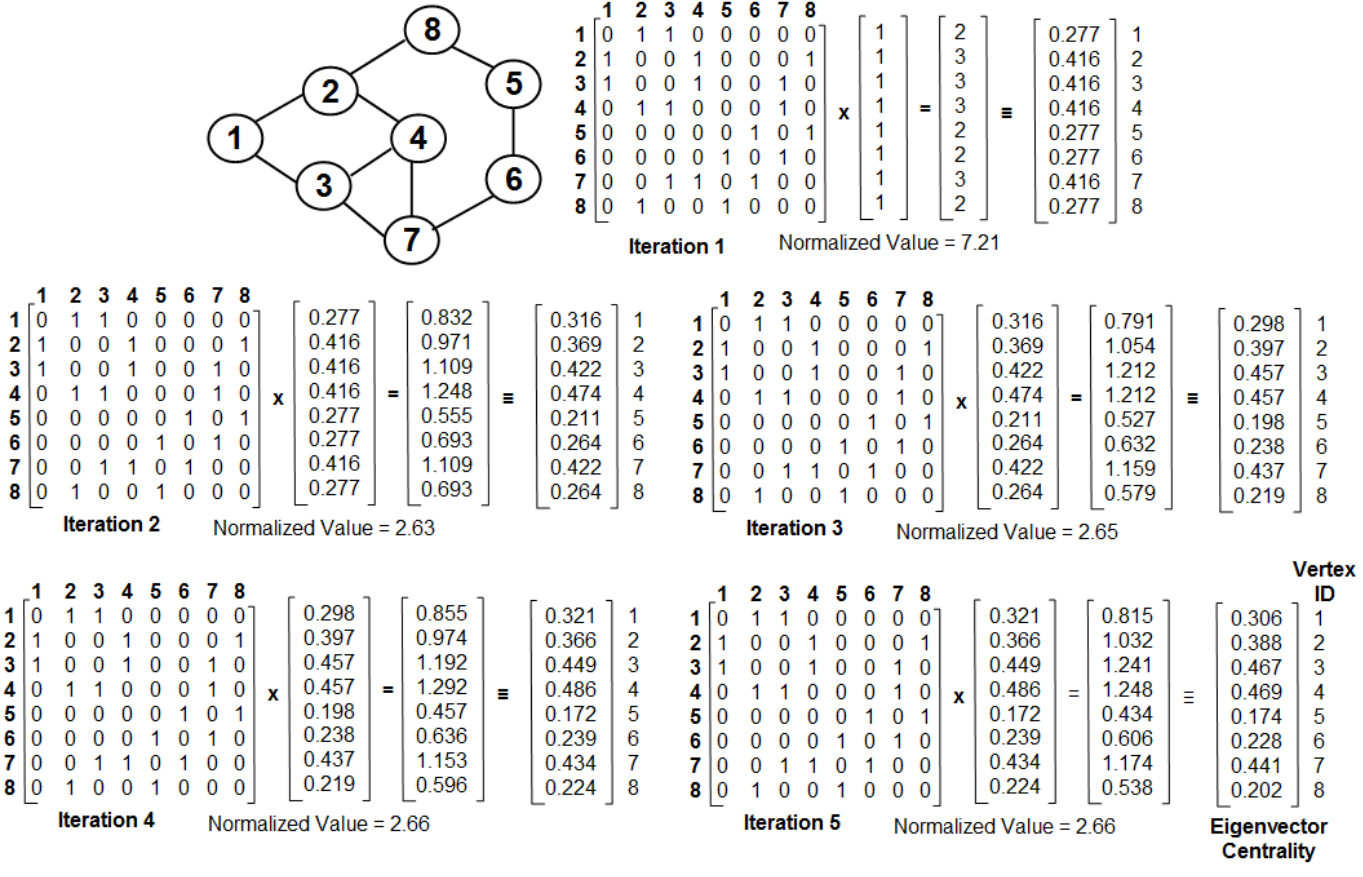
\includegraphics[scale=.32]{Abbildungen/eigenvektor_centrality_example.png}
	\caption[Eigenvektor Centrality: Power-iteration Method \cite{meghanathan_use_2015}]{Eigenvektor Centrality: Power-iteration Method \cite{meghanathan_use_2015}}
\end{figure}
Der limitierende Faktor dieser Methode zur Berechnung der "`Eigenvektor Centrality"' ist die Matrix-Multiplikation. Implementiert man diese naiv so ergibt sich eine Komplexität von \(O(n^3)\). Die Normierung lässt sich in linearer Laufzeit realisieren. Somit ist die Berechnung mit der "`Power-iteration method"' in polynominaler Laufzeit möglich. Die Metrik selbst lässt sich nativ in Wolfram und in Matlab finden. \cite{wolfram_graph_2020,matlab_measure_2020}
}
\subsubsection*{Page Rank}
{
Zum Abschluss der Zentralitätsmetriken soll eine Metrik dieser Kategorie vorgestellt werden, die einen hohen praktischen Nutzen findet. Der "`Page Rank"' oder die "`Page Rank Centrality"' beschreibt die Wichtigkeit eines Knotens auf Basis seines Ausgangsgrads, bzw. seiner Verbindungen zu anderen Knoten und des "`Page Ranks"' seiner benachbarten Knoten. Hierbei ähneln sich "`Page Rank"' und "`Eigenvektor Centrality"'. Die Metrik wurde erstmals in einem Google-Paper von Page und Brin veröffentlicht und soll Webseiten im World Wide Web bewerten. \cite{brin_anatomy_1998}

Es sei \(A\) eine Seite, bzw. ein Knoten und dieser Knoten hat Einwegkanten (Links) zu den Seiten \(T_1\dots T_n\). \(d\) sei ein frei wählbarer "`Dämpfungs"'-Faktor, der meist auf 0,85 gesetzt wird. Zudem ist \(C(A)\) als der Ausgangsgrad für eine Seite (Knoten) definiert. Der "`Page Rank"' ist dann folgendermaßen definiert.
\[
	PR(A) = (1-d)+d(\frac{PR(T_1)}{C(T_1)}+\dots +\frac{PR(T_n)}{C(T_n)})
\]
Die Berechnung des "`Page Ranks"' erfolgt durch einen iterativen Algorithmus, bei dem zunächst jedem Knoten der "`Page Rank"' \(1/|V|\) gegeben wird. Darauf aufbauend kann dann die obige Funktion zur weiteren Berechnung und die weiteren Iterationen herangenommen werden, bis die Metrik konvergiert. Der Algorithmus weißt dabei eine Zeit-Komplexität von \(O(k\cdot |E|)\) auf, wobei \(k\) für die Anzahl der Iterationen steht. \cite{oracle_pagerank_2017} "`Page Rank"' ist in allen angeführten Mathematikbibliotheken vertreten. \cite{sagemath_generic_nodate,wolfram_graph_2020,matlab_measure_2020}
}
\section{Chromatische Zahl und chromatischer Index}
{
Ein bekanntes Problem der Informatik ist das Färbeproblem. Es geht dabei darum einen Graphen so zu färben, sodass zwei benachbarte Knoten nicht die selbe Farbe haben. Anwendungen dafür kann man in vielen Problemen finden. Klassischerweise nimmt man das Beispiel der Karteneinfärbung, bei der jedes Land ein Knoten ist und die Karte so eingefärbt werden soll, dass zwei benachbarte Länder nicht die gleiche Farbe haben. Allerdings lässt sich das Färbeproblem auch auf andere relevantere Probleme anwenden. Man kann z.B. so auch einen konfliktfreien Stundenplan erstellen oder andere ähnliche Konflikt-Probleme lösen. Die Knotenfärbung eines Graphen selbst ist eine Abbildung \(c: V\mapsto S\), wobei S die Menge an möglichen Färbungen ist. \cite{diestel_graphentheorie_2000,aigner_graphentheorie_2015} 
}
\subsubsection*{Chromatische Zahl}
{
Auf Basis des Färbeproblems können eine Reihe an Metriken definiert werden. Betrachtet man das Problem mithilfe der Abbildungsfunktion \(c\), so ist der Graph korrekt gefärbt, wenn gilt: \(\forall v, w (v,w\in V \land \text{adjazent}(v, w)\implies c(v)\neq c(w))\). Die "`chromatische Zahl"' beschreibt nun die Mächtigkeit der minimalen Menge \(S\), für die diese Bedingung für den Graphen \(G\) zutreffen kann. Man bezeichnet die chromatische Zahl auch als \(\chi (G)\). Für einen leeren Graphen ist die chromatische Zahl 1. Liegt ein bipartiter Graph vor, so ist die chromatische Zahl offensichtlicherweise 2. \cite{diestel_graphentheorie_2000} Die chromatische Zahl kann sowohl von SageMath als auch von Wolfram berechnet werden \cite{sagemath_graph_2020-1,wolfram_wolfram_2020-1}

Das Herausfinden der chromatischen Zahl ist ein NP-vollständiges Problem und kann deshalb vermutlich auch nicht effizient berechnet werden. \cite{weisstein_chromatic_nodate,karp_reducibility_1996} So ist es möglich mittels eines Brute-Force-Algorithmus sämtliche Färbemöglichkeiten durchzuarbeiten und dann die Färbung herausnehmen, die gültig ist und die niedrigste Anzahl an Farben hat. Dieser Ansatz hätte eine exponentielle Laufzeit, die schon bei kleinen Graphen zu extrem hohen Rechenzeiten führen würde. Neben dieser naiven Variante werden u.a. auch heuristische Algorithmen genutzt, die versuchen die chromatische Zahl effizient zu approximieren. Ein Greedy-Algorithmus hierfür ist folgendermaßen in Pseudocode definiert:
\begin{lstlisting}
	Chromatic-Number(G(V, E))
		vertices <- sortiere_nach_Grad_absteigend(V)
		highestColor <- 1
		for (vertex in vertices)
			color <- lowestPossibleColor(G, vertex)
			vertex.color = color
			highestColor <- Max{highestColor, color}
		return highestColor
\end{lstlisting}
Dieser Algorithmus hat allerdings den Nachteil, dass es nur eine Annäherung an die chromatische Zahl ist und nicht gesichert ist, dass das Ergebnis korrekt ist. Seine Strategie besteht darin, den Graphen mit möglichst wenig Farben zu färben, indem zuerst die Knoten gefärbt werden, die die meisten Nachbarn haben. 
}
\subsubsection*{Chromatischer Index}
{
Neben der Markierung bzw. Färbung von Knoten, ist es auch möglich in einem Graphen Kanten zu färben. Hierbei ist ähnlich wie bei der Knotenfärbung gemeint, dass eine Kante aus der Menge \(E(G)\) auf eine Zahl, bzw. Farbe abgebildet wird: \(k: E\mapsto S\). Im Rahmen der Kantenfärbung ist es nun wichtig, dass zwei inzidente Kanten nicht die selbe Farbe zugewiesen bekommen. Das bedeutet, dass die Farben aller Kanten, die mit dem gleichen Knoten verbunden sind, eine unterschiedliche Farbe haben müssen. Formal lässt sich das mit der Funktion \(k\) so ausdrücken: \(\forall v,w(v,w\in E \land \text{inzident}\_\text{zu}\_\text{gleichem}\_\text{Knoten}(v,w)\implies k(v)\neq k(w))\). Findet man eine Abbildung, für die diese Bedingung zutrifft, so nennt man den Graphen \(k\)-Kanten-färbbar. \(k\) ist dabei die Mächtigkeit der Menge S, der gefundenen Abbildung. Das niedrigst mögliche \(k\) für einen Graphen ist dann dessen "`chromatischer Index"'. Man schreibt dafür auch \(\chi '(G)\). Der "`chromatische Index"' ist sowohl in Wolfram, als auch in SageMath verfügbar. \cite{andersen_edge-colorings_1977,sagemath_graph_2020-1,wolfram_wolfram_2020-1}

Jeder Graph fällt bei Betrachtung seines chromatisches Indexes in eine von zwei Klassen. Bei der ersten Klasse ist der chromatische Index \(\chi '(G)=\Delta(G)\), wobei \(\Delta(G)\) der Maximalgrad des Graphen ist. Fällt der Graph nicht in diese Klasse, so ist sein chromatischer Index \(\chi '(G)=\Delta(G)+1\). Obwohl dabei der chromatische Index sich pro Graph in einem extrem engen Korridor aufhält, ist die exakte Ermittlung des Indexes ein NP-vollständiges Problem und somit vermutlich nicht effizient, also in polynomialer Laufzeit, zu berechnen. Allerdings gibt es Spezialfälle, bei denen die Zuordnung des Graphen in einer der beiden Klassen einfach ist. So ist \(\chi '(G)=\Delta(G)\), wenn der Graph bipartit ist. Ist der Graph vollständig und die Anzahl der Knoten ist gerade, ist dies ebenfalls der Fall. Ein kompletter Graph mit ungerader Knotenanzahl hat dann logischerweise den chromatischen Index \(\chi '(G)=\Delta(G)+1\). \cite{plantholt_chromatic_1983}

Anwendung findet die Kantenfärbung in verschiedenen praktischen Problemen. Beispielsweise kann man es nutzen, um ein sogenanntes "`Round-Robin"'-Turnier mit möglichst wenig Runden zu planen. Ein "`Round-Robin"'-Turnier ist ein Turnier, bei dem jeder Teilnehmer auf jeden Teilnehmer einmal trifft. Dieses Problem ist zu lösen, indem jeder Teilnehmer durch einen Knoten repräsentiert wird und jede Begegnung durch eine Kante. Eine Farbe repräsentiert eine Runde. Werden die Kanten nun so gefärbt, dass der Turnier-Graph \(k\)-Kanten-gefärbt ist, hat man einen Turnier-Plan gefunden, der keine Konflikte hat. Ist der Graph zudem \(\chi '(G)\)-Kanten-gefärbt, so hat man den Plan gefunden, der möglichst wenig Runden erfordert. Der chromatische Index gibt in diesem Zusammenhang also an, wie viele Runden man minimal benötigt, sodass sich alle Teilnehmer einmal begegnen. Da der Graph bei dem sich alle einmal begegnen ein vollständiger Graph sein muss, ist auch schnell ersichtlich, wie viele Runden man braucht, betrachtet man die Ergebnisse des letzten Abschnitts. Neben "`Round-Robin"'-Turnieren lassen sich auch individuelle Turniere so planen. \cite{gross_handbook_2004}
}
\subsubsection*{Fraktionierte chromatische Zahl}
{
Neben der klassischen Art und Weise einen Graphen zu färben gibt es auch weitere Methoden. In der fraktionierten Graphentheorie ist es auch möglich, in einem Graphen seinen Knoten mehrere Farben zuzuweisen. Auf Basis dessen lassen wich weitere Metriken definieren, die die Graphenfärbung als Grundlage haben. Hierzu zählt die "`fraktionierte chromatische Zahl"'. Um diese Zahl zu definierten, ist zunächst zu klären, wie fraktionierte Färbung formal definiert werden kann. Eine \(b\)-fache Färbung eines Graphen weist jedem Knoten eine Menge an \(b\) Farben zu. Auch dies kann durch eine Abbildung dargestellt werden, indem ein Knoten auf eine Menge an Färbungen abgebildet wird. Bei der Färbung muss nun darauf geachtet werden, dass zwei adjazente Knoten mit ihren zugewiesenen Farben keine Schnittmenge bilden. Besser kann dies durch eine Funktion dargestellt werden. Sei \(A\) die Menge an verfügbaren Farben, so kann die Färbung mit folgendermaßen dargestellt werden: \(c: V\mapsto A^b\). Für die Graphen-Färbung muss nun gelten: \(\forall v,w(v,w\in V\land \text{adjazent}(v,w)\implies c(v)\cap c(w)=\emptyset)\). Für eine \(b\)-Färbung wird eine bestimmte Anzahl \(a\) an Farben benötigt. Zu einer solchen Färbung wird dann auch gesagt, dass es eine \(a:b\)-Färbung ist. Das niedrigste \(a\) für das ein Graph eine \(b\)-Färbung hat, nennt man die \(b\)-fache chromatische Zahl (\(\chi _b(G)\)). Dabei ist logischerweise \(\chi_1(G) = \chi (G)\). Die fraktionierte chromatische Zahl ist dabei im Gegensatz folgendermaßen definiert \cite{scheinerman_fractional_2011}:
\[\chi_f(G)=\lim_{b\to\infty}\frac{\chi_b(G)}{b}\]
Die fraktionierte chromatische Zahl ist also der Grenzwert für die \(b\)-fache chromatische Zahl geteilt durch \(b\), wenn \(b\) gegen unendlich geht. Im Gegensatz zur "`normalen"' chromatischen Zahl ist die fraktionierte chromatische Zahl eine rationale und keine natürliche Zahl. Die Berechnung der Metrik ist ein NP-vollständiges Problem. Allerdings gibt es für einige Graphen vorgefertigte Werte, die genutzt werden können. So ist die fraktionierte chromatische Zahl eines zyklischen Graphen \(C_{2n+1}\) z.B. \(2+(\frac{1}{n})\). Der Algorithmus zur Berechnung der Kennzahl bedient sich einem linearem Programm und ist äußerst schwer zu berechnen. Die Komplexität steigt exponentiell zur Ordnung des Graphen. Eine native Implementierung dazu findet sich in SageMath. Wie bei der normalen Färbung kann auch die fraktionierte Färbung für diverse konfliktfreie Planungen und dergleichen verwendet werden. \cite{weisstein_chromatic_nodate,sagemath_graph_2020-1,scheinerman_fractional_2011}
}
\subsubsection*{Fraktionierter chromatischer Index}
{
Wie es auch den chormatischen Index bei einerfacher Graph-Färbung gibt, ist auch ein fraktionierter chromatischer Index für einen Graphen \(G\) ermittelbar. Hierbei geht es auch um die Färbung von Kanten. Statt einer Kante nur eine Farbe zuzuordnen, werden ihr \(b\) Farben zugeordnet. Auch das lässt sich wieder als Funktion darstellen: \(k:E\mapsto A^b\). Ziel der Färbung ist es wieder, dass für zwei Kanten, die inzident zum selben Knoten sind, die Schnittmenge der Farben leer ist: \(\forall v,w(v,w\in E\land \text{inzident}\_\text{zu}\_\text{gleichem}\_\text{Knoten}(v,w)\implies k(v)\cap k(w)=\emptyset)\). Ein Graph ist nun \(a\)-fraktioniert-kantenfärbbar für eine \(b\)-Kantenfärbung, wenn es möglich ist mit \(a\) Farben eine \(b\)-Kantenfärbung für den Graphen \(G\) zu finden, für die die obige Bedingung zutrifft. Findet man für eine \(b\)-Kantenfärbung das kleinste \(a\) hat man die korrespondierende "`fraktionierte chromatische Kantenzahl"' \(\chi'_b(G)\) gefunden, wobei wieder gilt \(\chi'_1(G)=\chi'(G)\). Darauf aufbauend kann der "`fraktionierte chromatische Index"' \(X'_f(G)\) definiert werden \cite{weisstein_fractional_nodate-1,scheinerman_fractional_2011}:
\[
	X'_f(G)=\lim_{b\to\infty}\frac{X'_b(G)}{b}
\]
Die Berechnung ist allerdings aber auch anders möglich. Der fraktionierte chromatische Index kann nämlich mithilfe der fraktoinierten chromatischen Zahl berechnet werden. Es gilt: \(\chi'_f(G)=\chi_f(L(G))\). \(L(G)\) ist dabei der sogenannte korrespondierende Kantengraph von \(G\). Bei einem Kantengraph werden alle Kanten von \(G\) genommen und in Knoten umgewandelt. Waren dann in \(G\) zwei Kanten inzident zum gleichen Knoten werden sie im Kantengraph mit einer Kante verbunden.

Die Berechnung der Metrik ist in polynomialer Laufzeit möglich. Bei der Betrachtung der Mathematikbibliotheken kam heraus, dass die Metrik ausschließlich in SageMath vertreten ist. \cite{sagemath_graph_2020}
}
\section{Arborizität}
{
Ein wichtiger Teil der Graphentheorie ist die Betrachtung von Bäumen. Ein Baum ist eine Zusammenhangskomponente eines Waldes. Ein Wald wiederum ist ein Graph, der keine Zyklen aufweist. Mithilfe dieses Wissens kann eine weitere Metrik definiert werden. Betrachtet man einen Graphen, zusammenhängend oder nicht, kann man sich die Frage stellen, wie es möglich ist, diesen Graphen aus einer Menge an Wäldern zu erstellen. Wichtiger noch ist es herauszufinden, aus welcher minimalen Anzahl an Wäldern es möglich ist, den vorliegenden Graphen aufzubauen. Diese minimale Anzahl ist die "`Arborizität"'. Präziser ausgedrückt, ist die "`Arborizität"' von \(G\) (\(Y(G)\)) die minimale Anzahl an azyklischen Subgraphen (Wäldern), dessen Vereinigung \(G\) ergibt. Hierbei teilen sich die Subgraphen keine gemeinsamen Kanten. \cite{weisstein_arboricity_nodate}

Zur Berechnung der Arborizität lassen sich sowohl Spezialfälle ausmachen, aber auch eine allgemeine Berechnungsvorschrift finden. So ist es zunächst ersichtlich, dass ein bereits azyklischer Graph eine Arborizität von \(Y(G)=1\) hat. Ein vollständiger Graph \(K_n\) hat wiederum eine Arborizität von \(Y(K_n)=\ceil[\big]{n:2}\) und ein vollständig bipartiter Graph \(K_{m,n}\) weißt den Wert \(Y(K_{m,n})=\ceil[\big]{(mn):(m+n-1)}\) auf. Möchte man die Arborizität allgemein berechnen, ist ein bestimmter Parameter des Graphen zu berechnen. \(m_p\) gibt die maximale Anzahl an Kanten eines Subgraphen von \(G\) an, der \(p\) Knoten hat. Dieser Wert \(m_p\) muss nun für alle \(|G|>p>1\) berechnet werden. Mit dieser Berechnung lässt sich die Arborizität mit folgender Formel für jeden \(G\) ermitteln. \cite{weisstein_arboricity_nodate,nash-williams_edge-disjoint_1961}
\[Y(G)=\max_{p>1}\ceil[\Bigg]{\frac{m_p}{p-1}}\]
Die Berechnung der Arborizität ist in polynomialer Laufzeit möglich und kann in verschiedesten Szenarien angewandt werden. Einerseits kann es als Graph-Dichte-Maß herangezogen werden, da ein dichter, mit vielen Kanten durchzogener Graph, logischerweise eine höhere Arborizität aufweisen muss. Wie bereits in vorigen Kapiteln erwähnt, kann die Dichte für die Zuverlässigkeit bzw. Angriffssicherheit eines Netzwerks herangezogen werden. Weiterhin kann die Arborizität aber auch z.B. Aussagen über die Steifigkeit von Strukturen machen oder bei der Analyse von elektrischen Netzwerken helfen. Die Metrik ist in SageMath fest eingebaut. \cite{gabow_forests_1992,sagemath_graph_2020}

Die Spezialisierung der Arborizität ist die "`lineare Arborizität"'. Um diese Metrik zu definieren, muss zunächst der Begriff des "`linearen Waldes"' geklärt werden. Wie ein normaler Wald besteht ein linearer Wald ausschließlich aus azyklischen Graphen. Allerdings ist jede Zusammenhangskomponente des linearen Waldes ein Pfad. Man kann sich also einen linearen Wald graphisch als eine Ansammlung von vollständig unverzweigten Graphen vorstellen. Jeder Knoten hat nur ein oder zwei inzidente Kanten. Die "`lineare Arborizität"' \(la(G)\) ist nun analog zur normalen Arborizität die minimale Anzahl an linearen Wäldern, dessen Vereinigung \(G\) ergibt. \cite{alon_linear_1988}

Auch für die Berechnung dieser Metrik können Spezialfälle ausgemacht werden. Beispielsweise hat jeder \(d\)-reguläre Graph eine lineare Arborizität von \(\ceil[\big]{(d+1)/2}\). Außerdem konnte mithilfe des "`Linear Arboricity Conjecture"' bewiesen werden, dass für alle planaren Graphen gilt, dass die lineare Arborizität \(\ceil[\big]{\Delta :2}\) oder \(\ceil[\big]{(\Delta +1):2}\) ist. \(\Delta\) ist dabei der Maximalgrad von \(G\). Im Gegensatz zur normalen Arborizität ist die Ermittlung der linearen Arborizität nicht in polynomialer Laufzeit berechnenbar. Die Ermittlung dieser Metrik ist ein NP-vollständiges Problem. Die Kennzahl ist zudem in keiner er genannten Bibliotheken vorhanden. \cite{peroche_np-completeness_1984,calamoneri_planar_2010}
}
\section{Weitere Metriken}
{
Nachdem nun eine weite Reihe an Metriken vorgestellt wurde und diese jeweils in eine Kategorie eingeordnet wurden, sollen in diesem letzten Teil Graph-Kennzahlen vorgestellt werden, die nicht in eine der Kategorien passen aber dennoch Erwähnung finden sollen.
\subsubsection*{Unabhängigkeitszahl}
{
Bei der Betrachtung von Graphen ist es möglich sogenannte "`unabhängige"' Knotenmengen zu finden. Eine "`unabhängige"' Knotenmenge ist eine Untermenge \(S\) der Knoten \(V(G)\) (\(S\subseteq V(G)\)), sodass keiner der Knoten in \(S\) adjazent zu einem anderen adjazent ist. Betrachtet man beispielsweise einen bipartiten Graphen, so ist dessen Definiton so gestaltet, dass der Graph in zwei "`unabhängige"' Knotenmengen gegliedert werden kann. Um nun die sogenannte "`Unabhängigkeitszahl"' \(\alpha(G)\) für einen Graphen \(G\) zu ermitteln, muss man die größtmögliche "`unabhängige"' Knotenmenge für \(G\) finden. Die Mächtigkeit dieser Menge ist dann die "`Unabhängigkeitszahl"' von \(G\) \cite{diestel_graphentheorie_2000,weisstein_maximum_nodate,weisstein_maximum_nodate} Unterstützung für diese Metrik lässt sich SageMath und Wolfram direkt oder indirekt (Ausgabe der größten "`unabhängigen"' Knotenmenge) finden. \cite{sagemath_graph_2020,weisstein_independence_nodate}

Die Berechnung der "`Unabhängigkeitszahl"' erfolgt durch das finden der größten "`unabhängigen"' Knotenmenge. Dieses Problem ist NP-vollständig und lässt sich durch einen naiven Brute-Force-Algorithmus lösen. Dieser iteriert über jedes mögliche Subset von \(G\) und prüft, ob das Subset unabhängig ist. Ist über alle Untermengen iteriert worden, kann die Mächtigkeit der größten, unabhängigen Untermenge ermittelten werden. Die Zahl der zu untersuchenden Untermengen steigt exponentiell mit jedem weiteren Knoten. Durch Optimierungen und intelligente Algorithmen kann das Problem mittlerweile in einer Zeitkomplexität von \(O(1,1996^n)\) gelöst werden. Darüber hinaus gibt es neben exakten Algorithmen zur Ermittlung auch approximierende Algorithmen, die schneller sind. \cite{xiao_exact_2017}
}
\subsubsection*{Cliquenzahl}
{
Verwandt mit der Unabhängigkeitszahl ist die sogenannte "`Cliquenzahl"'. Wenn von Cliquen bei Graphen die Rede ist, ist eine Untermenge in einem Graphen \(G\) gemeint, in der jeder Knoten adjazent zu jedem anderen Knoten innerhalb der Untermenge ist. Deutlicher kann man es so ausdrücken, dass eine Clique in einem Graphen eine Untermenge an Knoten ist, die gemeinsam einen vollständigen Graphen bilden. Die Cliquenzahl \(\omega(G)\) ist nun die Mächtigkeit der größten Knotenmenge, die in G eine Clique formt. \cite{diestel_graphentheorie_2000} Auch die Cliquenzahl lässt sich in Wolfram und in SageMath finden \cite{wolfram_research_findclique_2015,sagemath_graph_2020} Das auffinden von Cliquen ("`Cliquenproblem"') und damit auch das ermitteln der Cliquenzahl ist ein NP-vollständiges Problem und kann deshalb vermutlich auch nicht effizient gelöst werden.

Das Prinzip der Clique kann, wie der Name schon nahelegt, beispielsweise auf sozialen Netze übertragen werden. Stellen Knoten Personen dar und Kanten Freundschaften, können durch das Auffinden von Graph-Cliquen echte Personen-Cliquen gefunden werden. Die Cliquenzahl eines Graphen gäbe in diesem Kontext dann Größe der größten Clique innerhalb eines sozialen Netzes an.
}
\subsubsection*{Buchdicke/Seitenzahl}
{
Als letztes soll noch eine geometrische Invariante untersucht und beschrieben werden: Die "`Buchdicke"' bzw. "`Seitenzahl"' \(bt(G)\) eines Graphen \(G\). Hierfür muss zunächst geklärt werden, was ein "`Buch"' im Rahmen der Graphentheorie ist. Ein \(n\)-Buch, bzw. ein "`Buch"' mit \(n\) Seiten, besteht aus einer Linie ("`spine"' oder "`Rücken"') \(L\), die sich in einem dreidimensionalen Raum aufhält und \(n\) Halb-Ebenen ("`Seiten"'), die L als ihre gemeinsame Grenze haben, an denen sie sich treffen. In ein solches Buch kann man einen Graphen hineinlegen. Hierbei liegt jeder Knoten auf dem "`Buchrücken"' \(L\) und jede Kante liegt auf einer der "`Seiten"'. Hierbei ist es wichtig, dass sich die Kanten auf einer Seite nicht kreuzen drüfen. Um dies besser zu verdeutlichen, wie sich dies graphisch wiederspiegelt sei Abbildung 2.2 gegeben. Gezeigt wird, wie ein vollständiger Graph mit fünf Knoten in ein Buch eingebettet wird.
\begin{figure}[ht!]
	\centering
	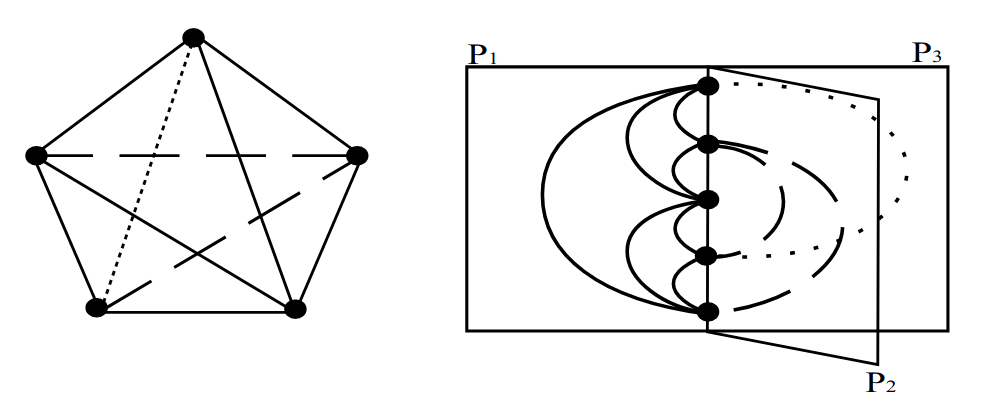
\includegraphics[scale=0.4]{Abbildungen/graph_book.png}
	\caption[Einbettung \(K_5\) in Buch \cite{blankenship_book_2003}]{Einbettung \(K_5\) in Buch \cite{blankenship_book_2003}}
\end{figure}
Die "`Buchdicke"' bzw. "`Seitenzahl"' \(bt(G)\) ist nun das kleinsmögliche \(n\) das gefunden werden kann, damit der Graph in das korrespondierende \(n\)-Buch hineingelegt werden kann. \cite{bernhart_book_1979} Die ermittlung von \(bt(G)\), bzw. das Entscheidungsproblem, ob ein Graph \(G\) in ein \(n\)-Buch eingebettet werden kann, ist ein NP-vollständiges Problem. \cite{chung_embedding_1987}

Die "`Buchdicke"' und das Einbetten von Graphen in ein "`Buch"' hat mehrere Anwendungsszenarien. Eines davon ist beispielsweise die Planung einer Ampelschaltung einer Kreuzung. Hierbei betrachtet man die Knoten eines Graphen als die ein- und ausgehenden Straßenspuren (inkl. Fuß- und Radwege). Die Kanten sind die möglichen Wege, die ich von einem Knoten zum anderen begehen/befahren kann. Die Knoten sind nun so auf dem "`Buchrücken"' zu arrangieren, dass ihre Reihenfolge auf dem "`Rücken"' der Reihenfolge der Spuren im Uhrzeigersinn auf der Kreuzung gleicht. Die Kanten werden anschließend in die "`Seiten"' eingebettet. Jede "`Seiten"' repräsentiert dann eine Ampelphase, die so geschaltet ist, dass die Verbindungen der jeweiligen Seite befahrbar sind, ohne das es zu Konflikten kommt. Die "`Buchdicke"' ist infolgedessen auch die minimal mögliche Anzahl an Ampelphasen an einer gegeben Kreuzung, die durch den Graphen G repräsentiert wird. \cite{kainen_book_1990}
}
\section{Übersicht der vorgestellten Graphmetriken}
{
Nachdem nun eine weite Reihe an Graph-Metriken vorgestellt wurden, sollen diese mit Hilfe einer Aufzählung zusammengefasst werden. Aufgelistet werden jeweils der Name, bzw die Bezeichnung, der Metrik und ihre Definition. Zudem soll klar werden in welche der Kategorien die Metrik gehört Bei der Definition wird dabei eine mathematische oder eine wörtliche Beschreibung angegeben. Gegebenenfalls auch beides, falls es für das Verständnis förderlich ist.

\metric{Ordnung \(|V(G)|\)}{Anzahl der Knoten eines Graphen}
\metric{Größe \(|V(E)|\)}{Anzahl der Kanten eines Graphen}
\metric{Knotengrad \(d(v)\)}{Anzahl der inzidenten Kanten des Knotens \(v\)}
\metric{Minimal- (\(\delta(G)\)) und Maximalgrad (\(\Delta(G)\))}{Der kleinste bzw. größte Knotengrads des Graphen \(G\); \(\delta (G):=min\{d(v)\ \vert\ v\ \in\ V(G)\}\), \(\Delta (G)\ :=\ max\{d(v)\ \vert\ v\ \in\ V(G)\}\)}
\metric{Anzahl der Zusammenhangskomponenten}{Anzahl der Komponenten/Subgraphen eines Graphen, die selbst zusammenhängend sind. Ein Graph (eine Komponente) ist dann zusammehängend, wenn sich zwischen zwei beliebigen seiner Knoten immer ein Weg finden lässt.}
\metric{Abstand/Distanz \(d_G(x,y)\)}{Die Länge des kürzesten Weges zwischen den beiden Knoten \(x\) und \(y\).}
\metric{Extrenzität eines Knotens \(ecc(x,G)\)}{Der Maximale Abstand, den ein Knoten zu einem anderen Knoten im Graphen \(G\) haben kann. \(ecc(x, G)=\max_{y\in V(G)}\{d_G(x,y)\}\)}
\metric{Durchmesser \(Duchmesser(G)\)}{Der größte Abstand zweier Knoten innerhalb des Graphen \(G\). \(Durchmesser(G)=\max_{x,y}\{ d_G (x,y)\}\).}
\metric{Radius \(rad(G)\)}{Kleinste Extrenzität innerhalb des Graphen. Extrenzität der Knoten des Zentrums. \(rad(G) = \min_{x\in V(G)}\max_{y\in V(G)}d_G(x,y)\).}
\metric{Taillenweite}{Länge des kürzesten Kreises innerhalb eines Graphen}
\metric{Umfang}{Länge des größten Kreises innerhalb eines Graphen}
\metric{Dichte}{Anzahl der Kanten des Graphen geteilt durch die Anzahl der möglichen Kanten. Ungerichteter Graph: \(\frac{\vert E\vert}{\binom{\vert V\vert}{2}}\). Gerichteter Graph: \(\frac{\vert E\vert}{2\binom{\vert V\vert}{2}}\)}
\metric{Stärke \(\sigma(G)\)}{Das Minimale Verhältnis zwischen entfernten Kanten und dadurch entstandenen Zusammenhangskomponenten. Sei \(\Pi\) die Menge aller möglichen Partitionierungen der Knoten \(V\) und \(\partial\pi\) die Menge an Kanten, die entfernt werden müssten, um die Partitionierung \(\pi\) zu erreichen, gilt folgende Formel zur Errechnung der Stärke:
\[\sigma(G)=\min_{\pi\in\Pi}\frac{\vert\partial\pi\vert}{\vert\pi\vert -1}\]}
\metric{"`Vertex Connectivity"'}{Minimale Anzahl \(k\) Knoten, die aus einem zusammenhängenden Graphen entfernt werden müssen, sodass er nicht mehr zusammenhängend ist.}
\metric{"`Edge Connectivity"'}{Minimale Anzahl \(k\) Kanten, die aus einem zusammenhängenden Graphen entfernt werden müssen, sodass er nicht mehr zusammenhängend ist.}
\metric{Degree Centrality}{Wichtigkeitsmaß für einen Knoten. Bewertet Knoten nach seinem Grad: \(d(v); v\in V\)}
\metric{Betweenness Centrality \(C_B(v)\)}{Wichtigkeitsmaß für einen Knoten, das angibt inwieweit beliebige kürzeste Wege zwischen zwei anderen Knoten durch ihn verlaufen. Sei \(\sigma_{st}\) Anzahl der kürzesten Wege zwischen Knoten \(s\) und \(t\) und \(\sigma_{st}(v)\) die Anzahl dieser Wege, die durch \(v\) laufen.
\[
	C_B(v)=\sum_{s\neq v\neq t\in V}\frac{\sigma_{st}(v)}{\sigma_{st}}
\]
}
\metric{Closeness Centrality \(C_C(v)\)}{Zentralitätsmetrik, die Knoten danach bewertet wie weit sie von jedem Anderen Knoten entfernt sind.
\[
	C_C(v)=\frac{|V|-1}{\sum_{u\in V}d_G(v,u)}	
\]
}
\metric{Eigenvektor Centrality \(x_v\)}{Zentralitätsmetrik, die einen Knoten dahingehend bewertet wie vernetzt er ist und wie vernetzt seine Nachbarn sind. Wendet man die Metrik auf die gesamte Adjazenzmatrix \(A\) an, so sind die Eigenvektor Centralities aller Knoten im Eigenvektor \(x\) zu finden, der nur positive Werte enthält.
\[
	x_v=\frac{1}{\lambda}\sum_{t\in M(v)}x_t=\frac{1}{\lambda}\sum_{t\in G}a_{v,t}x_t
\]
}
\metric{Page Rank \(PR(A)\)}{Praktisch angewandte Zentralitätsmetrik, die ähnlich wie die Eigenvektor Centrality einen Knoten nach seiner v+Vernetztheit und der Vernetztheit seiner Nachbarn bewertet. Sei \(A\) der zu untersuchende Knoten (Seite) und \(T_1\dots T_n\) die Knoten auf die von \(A\) aus gezeigt wird (Links), dass ist der Page Rank PR(A) so definiert:
\[
	PR(A) = (1-d)+d(\frac{PR(T_1)}{C(T_1)}+\dots +\frac{PR(T_n)}{C(T_n)})
\]
}
\metric{Chromatische Zahl \(\chi (G)\)}{Die minimale Anzahl an Farben mit denen es möglich ist die Knoten eines Graphen so zu färben, das keine zwei adjazenten Knoten die gleiche Farbe haben.}
\metric{Chromatischer Index \(\chi '(G)\)}{Die minimale Anzahl an Farben mit denen es möglich ist die Kanten eines Graphen so zu färben, das keine zwei inzidenten Kanten die gleiche Farbe haben.}
\metric{Fraktionierte chromatische Zahl \(\chi_f(X)\)}{Statt einem Knoten nur eine Farbe zuzuweisen, können ihm auch \(b\) Farben zugewiesen werden. \(\chi_b(G)\) gibt die minimale Zahl an unterschiedlichen Farben an, für die \(G\) so färbbar ist, dass zwei adjazente Knoten mit \(b\) Farben in ihren Farben eine leere Schnittmenge bilden. Die fraktionierte chromatische Zahl ist auf Basis dessen so formuliert:
\[\chi_f(G)=\lim_{b\to\infty}\frac{\chi_b(G)}{b}\]
}
\metric{Fraktionierter chromatischer Index \(\chi'_f(X)\)}{Statt einer Kante nur eine Farbe zu geben, können ihr auch \(b\) Farben gegeben werden. \(\chi'_b(G)\) gibt die minimale Zahl an unterschieldichen Farben an, für die \(G\) so färbbar ist, dass zwei zum gleichen Knoten inzidenten Kanten mit \(b\) Farben in ihren Farben eine leere Schnittmenge bilden. Der fraktionierte chromatische Index lässt sich daraufhin so formulieren:
\[
	X'_f(G)=\lim_{b\to\infty}\frac{X'_b(G)}{b}
\]
}
\metric{Arborizität \(Y(G)\)}{Minimale Anzahl an azyklischen Subgraphen (Wäldern), die zusammen wieder \(G\) ergeben. Sei \(m_p\) die maximale Anzahl an Kanten eines Subgraphen von \(G\) mit \(p\) Knoten, dann kann die Arborizität folgendermaßen berechnet werden:
\[Y(G)=\max_{p>1}\ceil[\Bigg]{\frac{m_p}{p-1}}\]
}
\metric{Lineare Arborizität \(la(G)\)}{Minimale Anzahl an Wäldern, die zusammen wieder \(G\) ergeben. Dabei sind die Zusammenhangskomponenten jedes Waldes ausschließlich Pfade.}
\metric{Unabhängigkeitszahl \(\alpha(G)\)}{Eine Knotenmenge ist dann unabhängig, wenn alle Knoten in ihr nicht adjazent zueinander sind. Die Mächtigkeit der größtmöglichen unabhängigen Knotenmenge ist die Unabhängigkeitszahl \(\alpha(G)\)}
\metric{Cliquenzahl \(\omega(G)\)}{Eine Clique ist eine Knoten-Untermenge von \(G\), die einen vollständigen Graphen ergebibt. Die Mächtigkeit der größtmöglichen Knoten-Untermenge von \(G\), die eine Clique ist, ist die Cliquenzahl \(\omega(G)\)}
\metric{Buchdicke/Seitenzahl \(bt(G)\)}{Ein Graph kann in ein Buch eingebettet werden, wobei die Knoten auf dem Buchrücken \(L\) angebracht sind und die Kanten über anliegende Seiten (Halbebenen) laufen und sich dabei nicht kreuzen dürfen. Die Buchdicke \(bt(G)\) gibt nun an, wie viele Seiten man für einen Graphen \(G\) braucht, um ihn in ein Buch einbetten zu können.}
}
\chapter{Implementierung und Umsetzung der Graph-Metriken}
{
Nachdem nun eine umfassende Anzahl an Graphmetriken besprochen wurde, ist es Ziel der Studienarbeit einen Teil dieser im Rahmen einer Klassenbibliothek umzusetzen. Die Entwicklung erfolgt dabei im Rahmen des klassischen Softwarelebenszyklus und besteht aus Anforderungsanalyse, Entwurf/Design, Implementierung und Testung/Überprüfung. \cite{balzert_lehrbuch_2009,balzert_lehrbuch_2011} Darüber hinaus soll auch die Algorithmik einzelner Metriken betrachtet werden und infolgedessen auf die Betrachtungen aus Kapitel 2 angeschlossen werden. Die implementierte Klassenbibliothek lässt sich auf \href{https://github.com/benedictweichselbaum/graph_metrics_class_library}{GitHub} finden und kann mittels der Versionierungssoftware "`Git"' kopiert werden. (URL: \url{https://github.com/benedictweichselbaum/graph_metrics_class_library})
}
\section{Anforderungsanalyse}
{
Im ersten Teil der Entwicklung sollen Anforderungen an die verschiedenen Softwareteile definiert werden. Unter Anforderungen (Requirements) werden dabei die Eigenschaften verstanden, die vom jeweiligen Softwaresystem erwartet werden. Zunächst wird definiert welche globalen Ziele die Implementierung der Graphmetriken verfolgt. Anschließend wird beschrieben, in welchen Rahmenbedingungen die Umsetzung stattfindet. Die Definition konkreter Anforderungen erfolgt im Anschluss und trennt sich in Anforderungen an die Graphdatenstruktur, auf der die Berechnungen stattfinden und in Anfordreungen an die eigentliche Berechung der Metriken. Es werden hierbei sowohl funktionale als auch nicht funktionale Anforderungen formuliert. Die hier durchgeführte Anforderungsanalyse orientiert sich bei den meisten Schritten an den aufgeführten Punkten und Schritten aus Helmut Balzerts "`Lehrbuch der Softwaretechnik"' und folgt dabei in vielen Gesichtspunkten der Anforderungsschablone der IEEE 830-1998. \cite{balzert_lehrbuch_2009,ieee_ieee_1998}
}
\subsection{Ziele der Graphmetriken-Implementierung}
{
Finales Ziel der Graphmetrik-Implementierung soll es sein, eine Klassenbibliothek zur Verfügug zu stellen, die es einem Anwender oder einer Anwenderin ermöglicht, mithilfe einer bereitgestellten Graphen-Datenstruktur, diverse Graphmetriken zu berechnen. Besonders wichtig und praxisrelevant sind dabei Kennzahlen zur "`Centrality"'. Dieses Hauptziel soll noch einmal in diese Unterziele untergliedert werden:
\singleenum{0}{Die Klassenbibliothek soll eine Graph-Datenstruktur bereitstellten, die einerseits die grundlegenden Operationen eines Graphen beherrscht und andererseits es ermöglicht die Berechungen für die Metriken auf ihr auszuführen. Dies ist nötig, da nur durch die Definition einer eigenen Datenstruktur eine Implementierung der Metriken möglich ist, da hierdurch zumindest der Zugriff auf den Graph standardtisiert ist.}
\singleenum{1}{Die Klassenbibliothek soll einen Mechanismus bereitsstellen, der es ermöglicht diverse Metriken für Graphen zu berechen. Die Berechnungen sollen dabei auf der vordefinierten Graph-Datenstruktur stattfinden, die zuvor definiert wurde. Dieses Ziel beschreibt die Hauptmotivation hinter dem Softwareprojekt.}
\singleenum{2}{Da es sich bei der Software um eine Klassenbibliothek handelt, ist es zudem zwingend notwendigt, dass die Bibliothek in andere Programme einbindbar ist. D.h. für einen anderern Entwicker oder eine Entwicklin muss es möglich sein, die Bibliothek in deren eigenen Programmen einzubinden und zu nutzen. Der letztendliche Sinn der Bibliothek soll es sein, das sie ggf. wiederauftretende Probleme im Zusammenhang mit Graphen lösen kann, ohne das ein Entwickler selbst eine Graphdatenstruktur oder die Metrik-Berechnung selbst implementieren muss. \cite{muller_vorkurs_2017}
}
\subsection{Rahmenbedingungen}
{
Durch die Zielformulierungen wurde auf einer abstrakten Ebene klar, was die zu erstellende Software können muss. Im folgenden soll geklärt werden, mit welchen Rahmenbedingungen die Klassenbibliothek erstellt werden soll. Es ist wichtig zu betrachten, welche Anwendungsbereiche das finale Produkt hat, wer die Zielgruppe ist und welche Betriebsbedingungen für die Bibliothek herrschen. Zudem müssen die technische Produktumgebung betrachtet und definiert werden. \cite{balzert_lehrbuch_2009}

Bei der Ermittlung des Anwendungsbereiches der Klassenbibliothek kann keine konkrete Räumlichkeit oder professionelle Arbeitsumgebung (writschaftlich oder akademisch) angegeben werden. Grundsätzlich ist der Anwendungsbereich dort, wo in einem Programm Graphen und Graphmetriken genutzt werden müssen. Wie bereits in Kapitel 1 erwähnt, ist der Graph und damit die zugehören Metriken vielverwendete Abstraktionen für viele Systeme. \cite{turau_algorithmische_2004} Damit ist auch der finale Anwendungsbereich einer solchen zugehörigen Bibliothek beliebig.

Da der Anwendungsbereich der Klassenbibliothek weit gefasst ist, besteht auch die potenzielle Zielgruppe aus vielen verschiedenen Personengruppen. Was diese Personen aber eint, ist, dass es sich immer um Softwareentwickler oder -entwicklerinnen handelt, da eine Klassenbibliothek immer im Rahmen einer anderen Software verwendet wird. In diesem Zusammenhang sei aber zu erwähnen, dass die zu entwickelnde Bibliothek vor allem im akademischen Kontext dieser Studienarbeit entsteht. Infolgedessen werden auch die realen Benutzer der Software sich in diesem Kontext bewegen.

Die Betriebsbedingungen der Bibliothek sind grundsätzlich beliebig. Die Ausführung der Programme kann auf jedem Computer geschehen, der die jeweiligen technischen Kriterien erfüllt, die anschließend in der technischen Produktumgebung beschreiben sind.

Die technische Produktumgebung ist folgendermaßen gegeben. Die Klassenbibliothek wird mittels der Programmiersprache \textbf{"`Java"'} umgesetzt. Das Softwareinkrement selbst wird mittels des Abhängigkeitsmanagementtools \textbf{"`Maven"'} "`gebaut"'. Durch Maven wird es auch möglich sein die erstellte Software in andere Projekte einzubinden.  Mit der Wahl von Java und Maven wird vorausgesetzt, dass der Endnutzer der Bibliothek die "`Java Virtual Machine"' installiert und einsatzbereit hat. Weitere Voraussetzungen sind nicht vorhanden. Die Auswahl von "`Java"' ist dadruch begründet, dass die Sprache sehr stark verbreitete und universell ausführbar ist, was u.a. dazu führte, dass es bereits einen großen Satz an Bibliotheken für die Sprache gibt. Das Verwenden von "`Maven"' als Abhängigkeitsmanagement- und Build-Tool ist dahingehend sinnvoll, da es einerseits speziell für Java entwickelt ist, andererseits wichtige Eigenschaften in Sachen Testing und Artefaktbereitstellung aufweist. So kann, wie bereits erläutert, die erstellte Bibliothek in anderen Proejkten mittels Maven eingebunden werden. \cite{ullenboom_java_2016,srirangan_apache_2011}
}
\subsection{Anforderungen an die Graphdatenstruktur}
{
Nachdem Ziel und Rahmenbedingungen des Softwareproduktes geklärt sind, müssen nun konkrete Anforderungen formuliert werden, die die Klassenbibliothek erfüllen soll. Im ersten Teil der Anforderungen wird bestimmt, welche Eigenschaften die Graph-Datenstruktur haben muss, die anschließend für die Berechnung der Metriken verwendet wird. Bei der Formulierung der Anforderungen wird natürliche Sprache verwendet. Zunächst werden funktionale Anforderungen beschrieben, anschließend nicht funktionale Anforderungen. \cite{balzert_lehrbuch_2009}

Vorrangig ist es wichtig, dass einem potenziellen Verwender bzw. einer potenziellen Verwenderin der Klassenbibliothek möglich gemacht wird, ein Objekt zur Verfügung zu haben, das einen Graphen repräsentiert. Genauer gesagt, muss die Bibliothek einem Programmierer oder einer Programmiererin, die diese verwendet, eine Möglichkeit geben, eine Datenstruktur zu erstellen, die einen Graphen repräsentiert. D.h. es wird eine Struktur geschaffen, die Knoten und Kanten kennt, wobei die Kanten eine Verbindung bzw. Beziehung zwischen Knoten darstellen. Besonders wichtig ist die Implementierung eines simplen und ungerichteten Graphen. Diese Anforderung korrespondiert direkt mit dem ersten Produktziel. Die Graph-Datenstruktur stellt den zentralen Einsprungspunkt dar, um mit der Bibliothek zu arbeiten und muss daher über eine leicht zu verstehende Schnittstelle oder Abstraktion zu erreichen sein. Dies bedeutet, dass der Zugriff auf das jeweilige Graphen-Objekt über eine einheitliche Schnittstelle erfolgt.

Darüber hinaus ist es wichtig neben der reinen Bereitstellung einer Datenstruktur auch zu definieren, welche Aktionen auf diese möglich sind. D.h. die Bibliothek muss es dem Nutzer oder der Nutzerin ermöglichen die Graphdatenstruktur zu benutzen. Zur Benutzung zählen die folgenden Aktionen bzw. Operationen:
\begin{myitemize}
	\item Das Hinzufügen eines Knotens.
	\item Das Löschen eines Knotens. Hierbei werden auch alle inzidenten Kanten gelöscht.
	\item Das Hinzufügen einer Kante.
	\item Das Löschen einer Kante.
\end{myitemize}
Auch diese Anforderung ist essentiell für die Erreichung des ersten Projektzieles. Die jeweiligen Operationen sind Teil der Graph-Schnittstelle, wie sie in der ersten Anforderung beschreiben wurde. Jedes Graph-Objekt kann über die Schnittstelle dementsprechend manipuliert werden.

Ein Graph dient meist zur Repräsentation und Abstraktion eines bestimmten Sachverhaltes \cite{turau_algorithmische_2004}. Viele Beispiele dazu konnten z.B. in Kapitel 2 gesehen werden, wobei unter anderem Anwendungen für Metriken besprochen und vorgestellt wurden. Auch die Graphdatenstruktur muss es ermöglichen, dass eine gewünschte Abstraktion dargestellt werden. Die Bibliothek muss es also ermöglichen Knoten und Kanten im Graphen zu "`markieren"'. Durch die Markierung muss es zudem möglich werden, die Knoten eindeutig zu identifizieren. Diese eindeutige Identifikation dient anschließend auch zur Durchführung der diversen Aktionen, die auf den Graphen möglich sind. Die verwendete Markierung soll dabei beliebig sein. Allerdings ist es notwendig, dass Markierungen untereinander vergleichbar sind, damit die Funktionalität des Graphen gewährleistet werden kann.

Neben dem Graphen selbst ist die Ermittlung diverser Metriken einer der Hauptziele der Klassenbibliothek. Um dies zu erreichen, ist es notwendig, dass ein Graph-Objekt es ermöglicht, Informationen über sich preis zu geben. Die Datenstruktur muss dementsprechend dem Nutzer oder der Nutzerin eine Möglichkeit zur Verfügung stellen, auf Informationen des Graphen zuzugreifen. Die Operationen, die hierfür nötig sind, sind die folgenden:
\begin{myitemize}
	\item Information, ob Graph einen bestimmten Knoten enthält.
	\item Inforamtion, ob Graph eine bestimmte Kante enthält.
	\item Herausgabe aller Knoten des Graphen.
	\item Herausgabe aller Kanten des Graphen.
	\item Auffinden eines Knotens über ein gleichwertiges Knoten-Objekt (nicht die gleiche Referenz)
	\item Auffinden aller Nachbarn eines Knotens
	\item Rückgabe einer Repräsentation des Graphen als Adjazenzmatrix.
\end{myitemize}
Die Eigenschaft, die diese Anforderung dem Softwareprodukt verleiht, ist schlussendlich die Bereitstellung sämtlicher nötigen Informationen, die für die Berechung der Metriken von Bedeutung sind.

Die nächste funktionale Anforderung an die Graphdatenstruktur hat mit der bereits beschriebenen Eigenschaft zu tun, dass die jeweiligen Graph-Objekte über eine einheitliche Schnittstelle erreichbar sind. Die Klassenbibliothek muss es explizit ermöglichen, dass der Programmierer oder die Programmiererin verschiedenartige Graphen mit der Bibliothek verwenden kann. D.h. die jeweilige Implementierung der Datenstruktur muss frei sein, während der Zugriff genormt ist. Infolgedessen ist es möglich verschiedene Implementierungen für den Graphen umzusetzten und zu nutzen. Die Bibliothek muss dabei selbst mindestens eine Implementierung bereitstellten. Sie sollte, wenn das möglich ist, mehrere Graphimplementierungen zur Verfügung stellen.

Die bisherigen Anforderungen beschrieben vor allem welche Funktionen der Graph selbst haben muss. Bei der Arbeit mit Graphen und den korrespondierenden Problemen ist es allerdings meist erforderlich oder erwünscht, dass es möglich ist einen Graphen zu persistieren und umgekehrt in das Programm und den Hauptspeicher zu laden. Deshalb muss die Klassenbibliothek auch ermöglichen einen beliebigen definierten Graphen in eine Datei eines bestimmten Formates zu speichern. Gleichermaßen müssen solche Dateien auch eingelesen werden können.
}
\subsection{Anforderungen an die Metriken-Berechnung}
{
Neben Definition der Eigenschaften der Graphdatenstruktur ist es nun möglich, Anforderungen zu definieren, die beschreiben, wie und welche Metriken berechnet werden. Bezug wird dabei auf die vorgestellten Metriken genommen, die in Kapitel 2 vorgestellt wurden. Da die Anzahl der Metriken allerdings verhältnismäßig hoch ist, werden im Zuge der Anforderungsformulierung Schwerpunkte gesetzt. Besonders wenig praktisch anwendbare Metriken sollen aus der implementierungstechnischen Betrachtung ausgeschlossen werden. Ein hohes Augenmerk soll auf die Zentralitätsmetriken gelegt werden (siehe Abschnitt 2.5).

Die erste funktionale Anforderung besteht darin, dass die Klassenbibliothek einen Mechanismus oder eine Struktur zur Verfügug stellen muss, die es dem Nutzer oder der Nutzerin ermöglichen Metrik-Kennzahlen aus einem erstellten Graphen zu extrahieren. Der Graph, der hierfür verwendet werden kann, ist durch die Schnittstelle vorgegeben, die im vorigen Kapitel erwähnt wurde. Mit dieser Anforderung ist nicht die Implementierung einer oder mehrerer konkreter Metriken gemeint, sondern der Entwurf eines Mechanismus, der bestimmt, wie die Metriken-Berechnung adressiert werden kann.

Auf Basis eines Mechanismus zur Berechnung der Graphmetriken muss definiert werden, welche Metriken die Klassenbibliothek berechnen soll. Hierbei sind zunächst die grundlegenden Metriken wichtig (siehe Abschnitt 2.1). Diese Metriken sind fundamentale Kennzahlen zur Beschreibung eines Graphen. Daher muss es die Bibliothek ermöglichen für einen Graphen diese grundlegenden Metriken zu berechnen. Dazu zählen die folgenden Kennzahlen:
\begin{myitemize}
	\item Ordnung (Order) eines Graphen
	\item Größe (Size) eines Graphen
	\item Knotengrad und zugehörig Minimal-, Maximal- und Durchschnittsgrad.
	\item Anzahl der Zusammenhangskomponenten 
\end{myitemize}

Neben diesen Basis-Metriken sind auch die Distanz-Metriken eine wichtige Menge an Kennzahlen, die für die Implementierung relevant sind. Besonders die kürzeste Distanz zwischen zwei Knoten ist äußerst wichtig, da die Kennzahl Basis für weitere Metriken ist, die auch Teil der Anforderungen sind. Aufgrunddessen muss die Bibliothek eine Berechungslogik bereitstellen, die es ermöglicht folgende Distanzmetriken zu berechnen:
\begin{myitemize}
	\item Minimale Distanz zwischen zwei Knoten
	\item Extrenzität eines Knotens
	\item Durchmesser
	\item Radius
\end{myitemize}

Wie anfangs beschrieben, sollen im Rahmen dieser Betrachtung die Zentralitätsmetriken besondere Betrachtung erfahren. In Kapitel 2 konnte gezeigt werden, dass diese Metriken besondere praktische Relevanz haben. So dienen sie z.B. zur Analyse in sozialen Netzen oder der Bewertung von Internetseiten. Infolgedessen muss die Klassenbibliothek dem Nutzer oder der Nutzerin es ermöglichen für einen Graphen die folgenden Zentralitätsmetriken zu berechnen:
\begin{myitemize}
	\item Degree Centrality
	\item Betweenness Centrality
	\item Closeness Centrality
	\item Eigenvector Centrality
	\item Page Rank
\end{myitemize}

Praktische Anwendung findet auch die Kennzahl der chromatischen Zahl. Darüber hinaus genießt das Färbeproblem Prominenz in der Informatik. Deshalb muss die Bibliothek die Berechung der chromatischen Zahl zur Verfügug stellen. Zudem soll es auch möglich sein den chromatischen Index zu ermitteln. In Kapitel 2.6 wurde auch gezeigt, dass es für die chromatische Zahl einen approximierenden Algorithmus gibt, der effizienter arbeitet als der klassiche Algorithmus. Auch dieser Algorithmus muss im Rahmen der Klassenbibliothek umgesetzt werden, damit der dem Entnutzer der der Endnutzerin zur Verfügug gestellt werden kann.

Um auch eine Metrik zur Verfügung zu haben, die Aussagen dazu trifft, wie stark der Graph zusammenhängt, muss die Klassenbibliothek auch eine Kennzahl dieser Kategorie berechnen können. Infolgedessen soll hierfür die "`Dichte"' eines Graphen berechenbar sein. 
}
\subsection{Nicht funktionale Anforderungen}
{
In den letzten zwei Abschnitten der Studienarbeit wurde erläutert und definiert, welche funktionalen Eigenschaften die Klassenbibliothek haben soll. Im Folgenden wird nun dargelegt, welche nicht funktionalen Eigenschaften die Software haben soll. Hierbei wurde sich an den Merkmalen des Standards ISO/IEC 9126-1 orientiert. \cite{balzert_lehrbuch_2009} Dieser Standard heißt in seiner aktuellsten Fassung ISO/IEC 25010:2011.

Die ersten nicht funktionalen Anforderungen beschäftigen sich mit dem Aspekt der "`Usability"'. Da es sich um kein Softwareprodukt mit einer Benutzeroberfläche handelt, wird der Aspekt der Usability im Bezug auf die Verwendung der Bibliothek durch einen Entwickler oder eine Entwicklering betrachtet. Hierbei sind besonders zwei Eigenschaften wichtig und relevant. Im Rahmen der Usability muss die Bibliothek beim Verwenden der Graphdatenstruktur und der Metriken darauf achten, dass der Nutzer oder die Nutzerin das System leicht versteht und gut bedienen kann \cite{balzert_lehrbuch_2009}. Dafür ist es besonders wichtig, dass darauf geachtet wird, wie Parameter, Felder und Methoden benannt sind. Aber auch die statische Struktur der Bibliothek muss einem logischen Aufbau folgen und konsistent sein. Sowohl die Verständlichkeit als auch die Bedienbarkeit eines Systems können auf die klassischen Usability-Eigenschaften übertragen werden, wie sie Jakob Nielsen in "`Usability Engineering"' beschreibt \cite{nielsen_usability_2010}. So fördert die Verständlichkeit eines Systems die Erlernbarkeit (\textit{Learnability}) und die Befriedigung (\textit{Satisfaction}). Die gute Bedienbarkeit geht wiederum mit einer erhöhten Benutzungs-Effizienz (\textit{Efficiency}) daher. Neben diesen Usability-Zielen ist es für eine Klassenbibliothek zudem unabdingbar, dass sie möglichst fehlerfrei ist (\textit{Errors}). Ohne diese Eigenschaft ist keine gute Usability zu erreichen, da ein Nutzer oder eine Nutzerin einer Klassenbibliothek davon ausgeht, dass die Programmlogik dieser möglichst fehlerfrei, bzw. vollständig fehlerfrei ist.

Auch die Eigenschaft, dass das Produkt die gewünschten Funktionalitäten bereitstellt, ist eine nicht funktionale Eigenschaften und soll selbstverständlich von der Klassenbibliothek erfüllt werden. Besonders die Eigenschaften der Agemessenheit und Genauigkeit sollen beachtet werden. Angemessenheit beschreibt die Fähigkeit einer Software geeignete Funktionen bereitzustellen, um die spezifizierte Aufgabe zu erledigen. Genauigkeit wiederum sagt aus, wie genau und akkurat die Software die Anforderungen erfüllt. Für beide Eigenschaften kann definiert werden, dass die Klassenbibliothek sowohl volle Angemessenheit als auch Genauigkeit für den Nutzer oder die Nutzerin liefern muss. Angemessenheit wird erreicht, wenn die formulierten Anforderungen wie beschrieben erfüllt werden. Die Genauigkeit der Software ist gegeben, wenn die jeweiligen Funktionen vollständig korrekt arbeiten.

Nicht nur muss die Funktionalität genau und angemessen bereitgestellt werden, sie muss auch effizient ausgeführt werden. Besonders zwei Punkte sind dabei bei Computerprogrammen interessant. Das Zeitverhalten und das Verbrauchsverhalten. Beim Verbrauchsverhalten ist u.a. die Auslastung der Ressource Arbeitsspeicher gemeint. Im Rahmen der Studienarbeit soll die Klassenbibliothek möglichst zeit- und ressourcenschonend sein. Allerdings geniesen beide Eigenschaften nicht höchste Priorität. Vor allem bei der Berechnung einiger Metriken kann es bei großen Graphen zu längeren Antwortzeiten kommen. Besonders bei NP-vollständigen Problemen ist die Berechnung unvermeidbar langsam.

Darüber hinaus ist auch die Wartbarkeit einen Systems äußerst wichtig, damit Änderungen und Fehlersuche- und Behebung erleichtert werden. Im Zuge der Wartbarkeit soll besonders die Eigenschaft der Testbarkeit hervorgehoben werden. Die Bibliothek muss eine hohe Testbarkeit aufweisen. D.h. speziell, dass besonders Methoden so konzipiert werden müssen, dass sie testbar sind. Nur so kann die Korrektheit der Algorithmen, die in der Klassenbibliothek Verwendung finden sichergestellt werden.

Eine weitere nicht funktionale Eigenschaft, die die Bibliothek mitbringen soll, ist die der Anpassbarkeit und Installierbarkeit. Beide Eigenschaften fallen unter den Oberbegriff der Portabilität. Darunter ist zu verstehen, dass die Software anpassbar und variabel in dem Sinne sein muss, als das sich das System gut an verschiedene Umgebungen und Anwendungsszenarien anpassen kann, damit die verwendende Person die Funktionen des Softwareprodukt vielfältig einsetzen kann. Eine gute Installierbarkeit wiederum beschreibt, dass im Rahmen der dokumentierten technischen Voraussetzungen die Software leicht installiert und verwendet werden können muss. Ist die Installierbarkeit nämlich nicht ausreichend gut, ist die Hürde zur Verwendung der Bibliothek zu hoch. 
}
\subsection{Nutzbarkeit als Klassenbibliothek}
{
Neben programmlogischen und nicht funkionalen Anforderungen ist noch eine Anforderung festzuhalten, die mit der Beschaffenheit als Klassenbibliothek der Software einhergeht. Nach dem dritten formulierten Software-Ziel ist festgeschrieben, dass im Sinne einer Bibliothek es möglich sein muss, diese innerhalb anderer Programme einzubinden. Auf Basis dessen lässt sich die Anforderung herausarbeiten, dass die Bibliothek für einen nutzenden Entwickler oder Entwicklerin in ein anderes Softwareprodukt einbinbar sein muss. In den Rahmenbedingungen wurde bereits festgelegt, dass diese Einbindung durch das Abhängigkeitsmanagementtool "`Maven"' geschehen soll. 
}
%% HIER WEITERMACHEN
\subsection{Use Cases der Klassenbibliothek}
{
Durch die Ermittlung und Formulierung der Anforderungen an die Klassenbibliothek zur Berechung von Graphmetriken, können diese auch in Use Cases überführt werden. Ein Use Case beschreibt und repräsentiert eine Sequenz von Aktionen, die ein Akteur in Interaktion mit dem Softwaresystem ausführen kann, um ein bestimmtes Ziel zu erreichen. Die formulierten Anforderungen werden nun also in Use Cases überführt. So ist es besser möglich zu sehen mit welchen Aktionen die Aktoren auf das System Metriken-Klassenbibliothek zugreifen. Auch wird klar, welche Funktionen die Klassenbibliothek gegenüber dem Aktor bietet. \cite{balzert_lehrbuch_2009}

Bei der Bestimmung der Aktoren kann sich diesem Fall nur eine Entität ausmachen lassen: Der Entwickler bzw. die Entwicklerin, die die Bibliothek potenziell nutzt, indem diese beispielweise in andere Softwareprodukte eingegliedert wird. Weitere Akteure gibt es nicht, da eine Bibliothek kein System ist, dass von anderen Endbenutzern direkt verwendet wird.

Bei Bestimmung der Use Cases muss definiert werden welche Aktionen der Aktor mit den System durchführen kann. Die erste Anforderungsbetrachtung erfolgte über die Graphdatenstruktur und was diese leisten können muss. Aus diesen Anforderungen können drei Use Cases ausgemacht werden, die noch weiter konkretisiert oder erweitert werden können.
\begin{myitemize}
	\item Graph erzeugen
	\item Graph manipulieren
	\item Graph analysieren
\end{myitemize}
Der Graph wird laut den Anforderungen über eine einheitliche Schnittstelle erreicht. Das bedeutet wiederum, dass der Use Case darum erweitert werden kann, dass eine bestimmte Graphimplementierung gewählt werden muss. Die Bibliothek erlaubt es auch auf Basis der Schnittstelle eine eigene Implementierung zu stellen, falls das vom Nutzer gewünscht ist. Der Use Case "`Graph manipulieren"' ist abstrakt und wird durch Use Cases konkretisiert, die die Manipulationen beschreiben. Dazu zählt die Löschung von Knoten und Kanten und das Einfügen von Knoten und Kanten. Da Markierungen für Kanten und Knoten ist jeweils als Use Case beim Einfügen inkludiert. Auch die Analyse des Graphen ist ein abstrakter Use Case. Abgeleitet aus den Funktionen, die die Bibliothek diesbezüglich leisten muss, können zwei Use Cases abgeleitet werden. Zum einen kann der Akteur die Existenz eines Graphelements erfragen, andererseits sich bestimmte Graphelemente zurückgeben lassen. Dazu zählen alle Knoten des Graphen, alle adjazenten Knoten eines Knoten und so weiter.

Neben den Use Cases zur Graphdatenstruktur können noch zwei weiterte Use Cases definiert werden. Ein zentraler und wichtiger Use Case ist die Berechung einer Metrik für einen Graphen. Die jeweiligen Metriken, die berechnet werden sollen, wurden bei den Anforderungen erwähnt. Ein weiterer Use Case ist das Einbinden der Klassenbibliothek in ein anderes Softwareprodukt. Die vorgestellten und definierten Use Cases werden im folgenden Use Case-Diagramm zusammengefasst (Abbildung 3.1).
\begin{figure}[ht!]
	\centering
	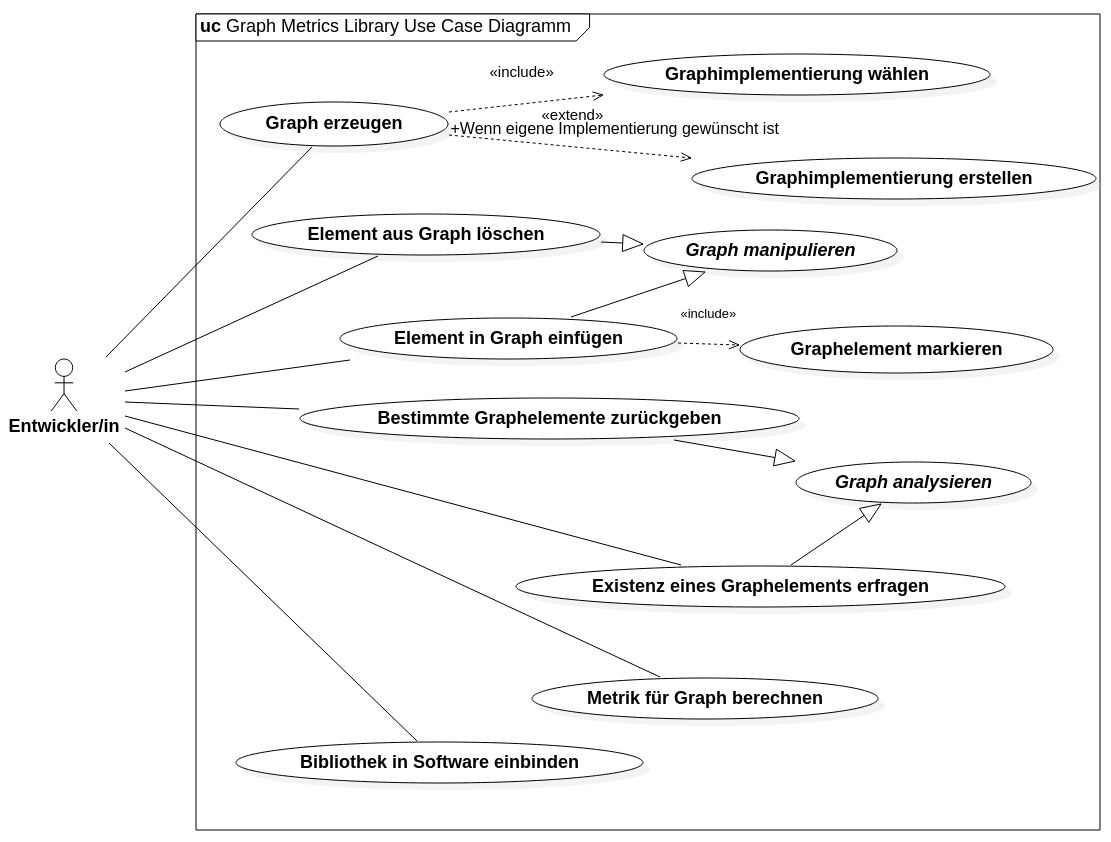
\includegraphics[scale=0.4]{Abbildungen/UML/library_use_case_diagram.png}
	\caption[Use Case-Diagramm: Graphmetriken-Klassenbibliothek]{Use Case-Diagramm: Graphmetriken-Klassenbibliothek}
\end{figure}

Für die mit dem Entwickler assoziierten Use Cases sollen noch Use Case-Schablonen formuliert werden \cite{balzert_lehrbuch_2009}:

\pagebreak
\usecase{Graph erzeugen}
{Ein Graphobjekt wurde innerhalb einer Variable\\oder eines Klassenfelds erzeugt.}
{-}
{Neues Graphobjekt in gewünschtem Wertebehälter}
{Fehlermeldung wird dem Nutzer oder der Nutzer-\\in gemeldet.}
{Entwickler/in}
{Entwicker oder Entwicklerin muss einen Graphen\\erstellen, der zur Repräsentation eines Sachver-\\halts dient.}
{Über einen Konstruktoraufruf wird ein neues Graph-\\objekt innerhalb eines Programms erstellt. Dabei\\muss eine bestimmte Graphimplementierung ge-\\wählt werden.}
{Ist eine andere Implementierung des Graphen ge-\\wünscht, kann auf Basis der vorgegebenen Schnitt-\\stelle eine eigene Implementierung erstellt werden.}

\usecase{Element aus Graph löschen}
{Ein Element wurde aus einem Graphobjekt ge-\\löscht.}
{Das zu löschende Element ist in Graph vor-\\handen.}
{Element nicht mehr in Graph vorhanden.}
{Fehlermeldung wird dem Nutzer oder der Nutzer-\\in gemeldet.}
{Entwickler/in}
{Entwickler/in will einen Knoten aus Graph\\löschen.}
{Über einen Zugriff auf das Graphobjekt wird\\ein Element identifiziert und gelöscht.}
{-}

\pagebreak
\usecase{Element in Graph einfügen}
{Ein Element wurde in ein Graphobjekt ein-\\gefügt.}
{Das zu löschende Element ist noch nicht im\\Graphen vorhanden.}
{Element ist im Graphobjekt vorhanden.}
{Fehlermeldung wird dem Nutzer oder der Nutzer-\\in gemeldet.}
{Entwickler/in}
{Entwickler/in will einen Knoten in Graph\\einfügen.}
{Über einen Zugriff auf das Graphobjekt wird\\ein neues Knotenobjekt eingefügt.}
{-}

\usecase{Bestimmte Graphelemente zurückgeben}
{Der Nutzer oder die Nutzerin konnte bestimmte\\Knoten und Kanten aus dem Graphen ex-\\trahieren.}
{-}
{-}
{-}
{Entwickler/in}
{Entwickler/in möchte Graph analysieren und Knoten\\ und Kanten extrahieren.}
{Um den Graph zu analysieren muss man auf seine\\Elemente über eine Schnittstelle zugreifen\\können. Hierzu zählt das Ausgeben aller Knoten,\\aller Kanten und eines bestimmten Knotens.}
{-}

\pagebreak
\usecase{Existenz eines Graphelements erfragen}
{Der Nuter oder die Nutzerin weiß, ob ein be-\\stimmter Knoten oder eine Kante im Graph\\existiert.}
{-}
{-}
{-}
{Entwickler/in}
{Die Entwickler/in möchte erfahren, ob ein\\Knoten oder eine Kante im Graph existiert.}
{Über die Graphschnittstelle ist es möglich\\zu erfragen, ob der Graph einen be-\\stimmten Knoten oder eine bestimmte Kante enthält.}
{-}

\usecase{Metrik für Graph berechnen}
{Der Nutzer oder die Nutzerin konnte sich vom\\Programm eine Metrik für einen\\bestimmten Graphen berechnen lassen.}
{-}
{Die korrekte Kennzahl wurde zurückgegeben.}
{Fehlermeldung wird dem Nutzer oder der Nutzer-\\in gemeldet.}
{Entwicker/in}
{Die Entwickler/in ist an einer Kennzahl für\\einen vorliegenden Graph interessiert.}
{Über die Berechnungslogik wird für einen\\Graphen eine vorgegebene Metrik berechnet.\\Das Ergebnis wird dem/der Entwickler/in\\zurückgemeldet.}
{-}

\pagebreak
\usecase{Bibliothek in Software einbinden}
{Der Entwickler bzw. die Entwicklerin, die\\die Bibliothek in eine Software einbin-\\den will, kann dies erfolgreich durchführen.}
{-}
{Bibliothek ist in ein anderes Software-\\produkt eingebunden.}
{-}
{Entwickler/in}
{Der/Die Entwickler/in möchte die Bibliothek\\in ein anders Softwareprojekt einbinden.}
{Durch den Einsatz von Maven ist es möglich\\die Klassenbibliothek in anderen Maven-\\projekten einzubinden und zu verwenden.\\Dafür muss das Artefakt als Abhängigkeit\\eingebunden werden.}
{-}
}
\section{Analyse zur Implementierung der Graphdatenstruktur}
{
Neber der Definition der Anforderungen und der Formulierung der Use Cases ist eine kurze Analyse über die Implementierung der Graphdatenstruktur notwendig. Weil es eine Reihe von möglichen Graphimplementierungen gibt, muss recherchiert werden, welche Implementierung für die Klassenbibliothek gewählt werden soll. Hierbei sei zu erwähnen, dass laut den Anforderungen die Klassenbibliothek grundsätzlich unabhängig von der konkreten Graphimplementierung arbeiten soll. Der Graph wird durch eine einheitliche Schnittstelle angesprochen. Allerdings ist aus den Anforderungen auch zu entnehmen, dass die Klassenbibliothek mindestens eine Implementierung liefern muss. Ziel ist es also herauszufinden, welche Implementierungen besonders relevant sind und umgesetzt werden sollen.

Bei der Wahl der Implementierung muss zunächst zwischen Graphart und der repräsentierenden Datenstruktur unterschieden werden. Ersteres beschreibt die Art und Weise wie der Graph agiert und was in ihm möglich ist, wenn man ihn manipuliert. Hier kann eine Unterscheidung zwischen einem simplen und nicht simplen Graph vorgenommen werden. Auch wird festgelegt, ob der Graph gerichtet ist oder nicht. Außerdem können sich Graphen dahingehend unterscheiden, dass sie Markierungen zulassen oder nicht. Bei der in Kapitel 2 vorgestellten Metriken wurde hauptsächlich auf simple, ungerichtete Grphen eingegangen. Aufgrunddessen soll auch die Standardimplementierung in der Klassenbibliothek einen solchen Graphen umsetzten. Dies bedeutet, dass beim Einfügen von Kanten darauf geachtet werden muss, dass eine Kante nicht bereits eingefügt worden ist und eine Kante immer in beide Richtungen eingefügt werden muss. Bei der Löschung einer Kante ist im Gegenzug darauf zu achten, das jeder Eintrag gelöscht wird, der die jeweilige Kante rerpäsentiert. Da allerdings einige Metriken und auch Graph-Anwendungsfälle auf gerichtete Graphen setzten, soll auch eine Implementierung für einen solchen Graphen erfolgen. Die Implementierung beim Einfügen und Entfernen von Kanten muss dementsprechend anders sein. Aus den Anforderungen geht weiterhin heraus, dass ein Graph meist einen bestimmten Sachverhalt wiederspiegelt und deshalb markierbar sein muss. Dies begründet auch, dass die Graphimplementierung in der Klassenbibliothek Markierungen zulässt.

Zur Wahl der Datenstruktur muss zunächst betrachtet werden, welche Möglichkeiten es gibt, einen Graphen zu repräsentieren, wenn man ihn programmatisch im Arbeitsspeicher darstellt. Grundsätzlich lassen sich vier Datenstrukturen ausmachen \cite{knebl_algorithmen_2019}:
\begin{myitemize}
	\item Adjazenzmatrix
	\item Adjazenzlisten
	\item Inzidenzmatrix
	\item Inzidenzliste
\end{myitemize}
Alle diese Datenstrukturen bringen ihre eigenen Vor- und Nachteile mit sich. Besonders bei den verschiedenen Einfüge-, Lösch- und Abfrageoperationen weisen die jeweiligen Implementierungen Unterschiede auf. Auch beim Speicherverhalten sind starke Unterschiede auszumachen.

Die Adjazenzmatrix ist eine sehr einfache Art und Weise einen Graph umzusetzten. Eine Markierung der Knoten und der Kanten ist mit ihr möglich. Besonders das Einfügen einer Kante ist in der Matrix sehr schnell und in konstanter Zeit möglich, da nur die Knotenindices addressiert werden müssen. Gleich verhält es sich für das Löschen einer Kante. Im Gegenzug ist allerdings das Einfügen und Löschen eines Knotens äußerst aufwendig. Da eine Adjazenzmatrix meist über Arrays realisiert wird, muss beim Einfügen und Löschen eines Knotens eine neue größere oder kleinere Martix initialisiert werden, in die dann alle vorigen Werte der alten Martix kopiert werden müssen. Ein weiterer schwerwiegender Nachteil der Matrix ist, das diese oft dünn besetzt ist, da Graphen selten vollständig sind. Dadurch wird äußerst viel Speicherplatz verschwendet. Dies ist besonders kritisch, da der Speicherbedarf der Matrix quadratisch mit der Anzahl der Knoten steigt.

Anders verhält sich das bei den Adjazenzlisten. Das einfügen eines Knotens ist hier sehr einfach möglich, da nur eine neue Liste angelegt werden muss, die an den neuen Knoten gebunden ist. Auch beim Einfügen einer Kante ist die Adjazenzliste leicht zu manipulieren, da nur in eine oder mehrere der Listen ein Eintrag hinzugefügt werden muss. Ähnlich verhält es sich beim Löschen von Knoten und Kanten. Bei der Kantenlöschung müssen nur die entsprechenden Einträge aus den Adjazenzlisten gelöscht werden. Bei der Knotenlöschung kann die entsprechende Liste vollständig gelöscht werden und die übrigen Kanteneinträge aus den anderen Listen werden auch entfernt. Beim Speicherverhalten verbraucht die Adjazenzliste nur so viel, wie der Graph Informationen trägt. Der Verbraucht steigt also linear mit Knoten- und Kantenanzahl.

Inzidenzliste- und Matrix repräsentieren den Graphen durch das aneinanderreihen von Kanten und ihren Informationen (inzidente Knoten). Dadurch sind Kanteneinfüge- und löschoperationen leicht zu realisieren. Allerdings ist man bei der Matrix durch ihre festgelegte Größte stärker beschränkt und muss beim Löschen und Einfügen die Matrix neu initialisieren. Der Speicherbedarf steigt linear bei beiden Lösungen mit der Anzahl der Kanten. Bei der Inzidenzmatrix wird die Matrix zudem linear größer, desto mehr Knoten im Graphen sind.

Neben den manipulierenden Operationen auf die Datenstrukturen sind auch analysierende Zugriffe wichtig zu betrachten. Hier stellt sich heraus, dass die adjazenz-basierten Datenstrukturen sich besser zur Informationsbeschaffung eignen als die inzidenz-basierten. Besonders die Adjazenzliste ermöglicht es einfach die Nachbarn eines Knotens auszugeben. Soll die Nachbarschaft zweier Knoten nachgewiesen werden, ist die Matrix zwar am schnellsten, die Liste schafft es aber dennoch in linearer Zeit. Bei den inzidenz-basieren Strukturen sind vor allem lesende Operationen günstig, die die Inzidenz aufzeigen wollen. \cite{bettilyon_implementations_2019}

Aufgrund der guten Speicherverbrauchseigenschaften und der relativen Einfachheit der Manipulation soll für die Klassenbibliothek der Graph mittels Adjazenzlisten implementiert werden. Zudem sind die Adjazenzlisten günstig, da sie sich leicht auswerten lassen. Besonders bei Nachbarschaftsbeziehungen ist dies der Fall. Bedenkt man, dass für die Berechnung der Metriken besonders die Auswertung des Graphen wichtig ist, wird die Wahl noch einmal untermauert. So werden beispielsweise bei der chromatischen Zahl oder beim Page Rank die adjazenten Knoten eines Knotens immer wieder benötigt.
}

\section{Analyse zur Persistierung des Graphs}
{
Um einen Graphen innerhalb einer Datei zu persistieren, gibt es eine weite Reihe an Möglichkeiten und Formaten. Es soll deshalb diskutiert werden, welche Persistierungsform für die zu umsetzende Klassenbibliothek gewählt werden soll.

Die Darstellung von Graphen in Textform wurde bereits von vielen Datenformaten unternommen. Dabei werden eigene Textformate verwendet oder auf bewährte Formate wie XML, CSV und JSON zurückgegriffen. Vertreter dieser bereits existenten Formate sind z.B. das \textit{"`Graph Exchange XML Format"'}, \textit{"`GDF"'} oder \textit{"`CSV"'}. \cite{gephi_supported_2017} Weiterhin ist das Feld der Graph-Textformate allerdings immer noch im Wandel und so gibt es weiterhin auch neue Ansätze. So wurde 2021 von Adreas Kollegger, einem Mitarbeiter von Neo4j Inc., ein weiteres Format namens "`gram"' vorgeschlagen. Dieses Format kombiniert Elemente des JSON-Formats und der Abfragesprache Cypher, die für Anfragen an die Graphdatenbank Neo4j genutzt wird. So können Knoten-Objekte über die JSON-Syntax definiert werden und Kanten zwischen diesen Knoten über eine Cypher-artige Syntax erstellt werden (z.B. \textit{(a: A)-[:Mark]-\(>\)(b: B)}). \cite{kollegger_gram_2021}

Für die Persistierung innerhalb der Klassenbibliothek soll sich nun auch an diesem "`gram"'-Format orientiert werden. Hierfür wird zunächst in der Datei angegeben, ob es sich um einen gerichteten oder um einen ungerichteten Graphen handelt. Anschließend werden wie in "`gram"' die Graphobjekte (Knoten \textbf{und} Kanten) über JSON definiert und bekommen einen Identifier. Zum Schluss des Dokuments werden die einzelnen Beziehungen, wie bereits gezeigt, einzeln aufgeführt. Mithilfe der erweiterten Backus–Naur Form, können die Ableitungsregeln der definierten Grammatik der Format-Sprache folgendermaßen dargestellt werden. Hierbei werden bestimmte Ableitungen abgekürzt. So beschreibt das Nicht-Terminal "`JSON"' die normale JSON-Sytax. Das Startsymbol ist "`graph"':
\begin{verbatim}
	graph = ('directed' | 'undirected'), '\n', {object}, {connection};
	object = '(', IDENTIFIER, JSON, ')', '\n';
	connection = '(', IDENTIFIER, ')', '-[', IDENTIFIER, ']->', 
		'(', IDENTIFIER, ')', '\n';
\end{verbatim}
Das definierte Format bietet nicht nur den Vorteil, dass beliebige Graphen intuitiv gespeichert werden können, sondern kann auch einfach Implementiert werden, da die Erstellung von JSON-Strings durch Bibliotheken wie "`Jackson"' übernommen werden kann.
}
\section{Entwurf der Klassenbibliothek}
{
Auf Basis der der Anforderungen und der angefertigten Analysen wird nun ein Entwurf erarbeitet, der die geforderten Anforderungen umsetzt. Dabei wird vor allem auf die Struktur und Dynamik der Klassenbibliothek eingegangen. Es soll hervorgehen, wie die Bibliothek konzipiert ist und auch wie sie effektiv genutzt werden kann. Anschließend wird als Teil des detailierten Entwurfs auch auf die konkrete Algorithmik der Graphmetriken eingegangen. \cite{balzert_lehrbuch_2011}

Im ersten Teil der jeweiligen Entwurfsbeschreibung (Statik und Dynamik) geht es um die Umsetzung und Implementierung zu den Anforderungen der Graphdatenstruktur. Im Zuge dessen werden auch die Use Cases "`Graph erzeugen"', "`Graph manipulieren"' und "`Graph analysieren"' umsetzt. Im zweiten Teil, wird jeweils darauf eingegangen, wie die Berechnung der Metirken umgesetzt wird.
}
\subsection{Statischer Entwurf}
{
Zunächst soll ein statischer Entwurf der Klassenbibliothek angegeben werden. Der statische Entwurf beschreibt die Struktur der Software und damit den Teil, der sich zur Laufzeit einer Programms nicht ändert. Durch den statischen Entwurf soll vor allem klar werden, wie die Klassenbibliothek verwendet werden kann, indem die relevanten Schnittstellenklassen identifiziert und beschrieben werden.

Im Rahmen dieses Entwurfes wird vor allem auf die Beschreibung durch Klassen zurückgegriffen. Das finale Ergebnis stellt auch stehts ein Klassendiagramm dar.
}
\subsubsection*{Graphdatenstruktur}
{
Um die Graphdatenstrukur zur Verfügung zu stellen, sind zwei Dinge notwendig. Zunächst muss eine Schnittstelle für ein Graphobjekt definiert werden. Danach ist es nötig eine Implementierung für diese Schnittstelle zu definieren. Teil der Schnittstelle sind alle nötigen Methoden, die in den Anforderungen definiert wurden. Dazu zählen die manipulierenden und analysierenden Operationen. Dadurch, dass der Graph durch eine Schnittstelle definiert wird, ist auch direkt gewährleistet, dass ein anderer Programmierer oder eine andere Programmiererin eine eigene Graph-Datenstruktur entwickeln kann. Er oder sie muss dafür nur die definierte Schnittstelle implementieren.

Weiterhin muss es ermöglicht werden, dass die zu erstellenden Graphen markiert werden müssen. Hierbei muss eine Markierung am Knoten und an den Kanten möglich sein. Damit die Markierung vollkommen frei wählbar ist, wird für den Graphen parametrisierte Polymorphie angewandt. D.h. im speziellen, dass das definierte Interface für den Graphen generifiziert wird über zwei Typvariablen. Die erste Typvariable gibt dabei den Typen der Knotenmarkierung an, die zweite den Typen der Kantenmarkierung. Da es laut den Anforderungen verpflichtend ist, dass ein Knoten im Graphen über seine Markierung identifiziert wird, ist es zudem notwendig, den Typparameter für die Knotenmarkierung einzugrenzen. Speziell ist es notwendig, dass Knotenmarkierungen vergleichbar sind. Um dies zu gewährleisten wird festgelegt, dass alle Knotenmarkierungstypen das Interface \textit{Comparable} implementieren. Dieses Interface ist dabei schon Teil der Java Standard-Bibliothek \cite{oracle_java_2021}. Durch diese Einschränkgung wird es möglich, dass Knoten untereinander vergleichbar werden, da über die Methode \textit{compareTo} ein Abgleich stattfinden kann.

Da Kanten nicht wie Knoten ausschließlich über ihre Markierung beschreiben werden können, ist es notwendig eine eiegne Kantenklasse zu definieren. Diese ist ein einfaches Java-Objekt (POJO) bestehend aus dem Ausgangsknoten, dem Eingangsknoten und der Markierung.

Auf Basis von Kapitel 3.2 wurde klar, welche Grapharten implementiert werden sollen. Umgesetzt werden zwei simple Adjazenzlistengraphen. Einer davon ist gerichtet, der andere nicht. Da sich beide Implementierungen bis auf die Handhabung mit Kanten gleichen, ist es sinnvoll eine Abstraktionsebene in die Umsetzung einzubauen. So implementiert eine abstrakte Klasse \textit{AdjacencyListGraph} das Graph-Interface und definiert alle Methoden bis auf das Einfügen, Löschen und Existenzabfragen von Kanten. Durch die abstrakte Klasse ist es möglich Codewiederholungen zu vermeiden, da Code für die jeweiligen Grapharten wiederverwendet werden kann. Zur eigentlichen umsetzung der Adjazenzlisten nutzt \textit{AdjacencyListGraph} eine Java-Map, wobei als Instantzobjekt eine Hash-Map verwendet wird. Die Map hat den Typen \textit{Map\textless N, List\textless Edge\textless N, E\textgreater\textgreater\textgreater}, wobei \textit{N \& E} die generischen Typparameter für den Knoten und die Kantenmarkierung sind. Wie zu erkennen ist, wird ein Knoten auf seine jeweilige Adjazenzliste abgebildet. Die Map ist einer geschachtelten Liste überlegen, da die Suche nach der jeweiligen Adjazenzliste in konstanter Zeit möglich ist, anstatt eine ganze Liste zu durchsuchen. Zudem ist die Zuordung des Knoten zu seiner Liste bereits in der Datenstruktur integriert.

Für manche Graphmetriken ist es relevant welche Graphart vorliegt. So ist z.B., wie in Kapitel 2 gezeigt, die Berechnung der Dichte abghängig davon, ob ein gerichteter oder ein ungerichteter Graph vorliegt. Um bei der Metrikenberechnung eine Unterscheidung zwischen den Arten treffen zu können, ist es nötig diese zu markieren. Hierfür wird sich sogenannter "`Marker-Interfaces"' bedient. Diese beinhalten keine Methoden und können so beliebig von Klassen "`implementiert"' werden. Im Falle der Klassenbibliothek gibt es die vier Marker-Interfaces \textit{SimpleGraph}, \textit{NonSimpleGraph}, \textit{DirectedGraph} und \textit{UndirectedGraph}. Die beiden Graphimplementierungen "`implementieren"' dann ihre jeweiligen Schnittstellen. Innerhalb von Java kann dann mit einer \textit{instanceof}-Abfrage erfragt werden, um welche Art von Graph es sich handelt.

Auch wenn die Bibliothek keine direkte Implementierung des Graphen über eine Adjazenzmatrix bereitstellt, ist die Repräsentation durch diese für eine Metrik relevant. Die Eigenvector Centrality benötigt zur Berechnung über die "`Power Iteration"' die Adjazenzmatrix. Infolgedessen muss noch eine weitere Klasse hinzugefügt werden, die die Klassenrepräsentation übernimmt. Da keine Manipulation dieser Matrix vorgesehen ist, bietet sie nur einen Konstrktor zum Aufbau der Datenstruktur. Hierbei hält die Klasse \textit{AdjacencyMatrix} eine Map, die einen Knoten auf seinen Matrix-Index abbildet und die Matrix selbst, die die Kantenmarkierungen enthält.

Um die Anforderung zur Persistierung des Graphen zu erfüllen, muss eine weitere Klasse zur Verfügung gestellt werden. Diese hält zwei statische Methoden, die einen Graphen persitieren bzw. laden können. Hierbei kann ein freier Dateipfad gewählt werden.

Außerhalb der Klassen, die zur Erfüllung der Anforderungen dienen, wurde zudem eine Klasse erstellt, die nur statische Methoden enthält, die dazu bestimmt sind, Standard-Graphen zu erstellen. Dies ist vor allem für das spätere Testen relevant, da so die Grapherstellung bei den Tests erleichert wird und einige Metriken bekannte Werte für diese Standardgraphen haben. Zur den verfügbaren Graphen gehören der vollständige Graph, der vollständig bipartite Graph, der Kreisgraph und der Liniengraph.

Schlussendlich ist es im Rahmen der Implementierung noch wichtig sich, um mögliche Fehler und Ausnahmen zu kümmern. Hierfür stellt die Klassenbibliothek im Rahmen der Graphdatenstruktur drei eigene Exceptions zur Verfügung. Die \textit{GraphManipulationException} wird geworfen, wenn bei der Graphmanipulation entwas illegales passiert. Dies ist z.B. der Fall, wenn ein gleicher Knoten zum zweiten Mal eingefügt wird. Die \textit{GraphCreationException} wird genutzt, wenn bei der Standardgrapherstellung etwas schief läuft. Die \textit{GraphAnalyticException} wiederum wird geworfen, wenn bei der Graph-Analyse ein Fehler auftritt. Ein Beispiel hierfür ist die Abfrage nach den adjazenten Knoten eines Knotens, der nicht im Graph existiert.

Durch die oben angegebene Menge an Klassen und Methoden können nun alle funktionalen Anforderungen aus 3.1.3 umgesetzt werden. Es wird eine markierbare Graphdatenstruktur als Schnittstelle vorgegeben und zwei Implementierungen für diese bereitgestellt. Durch die Schnittstelle wird aber einem fremden Entwickler bzw. einer fremden Entwicklerin die Freiheit gelassen, eine eigene Implementierung zu nutzen. Weiterhin ist die Persistierung und das Laden von Graphen mittels Textdateien möglich.

Die beschriebenen Klassen und Methoden zur Graphdatenstruktur können übersicht-lich mittels des Klassendiagramms in Abbildung 3.2 zusammengefasst werden.
\begin{landscape}
	\begin{figure}[p]
		\centering
		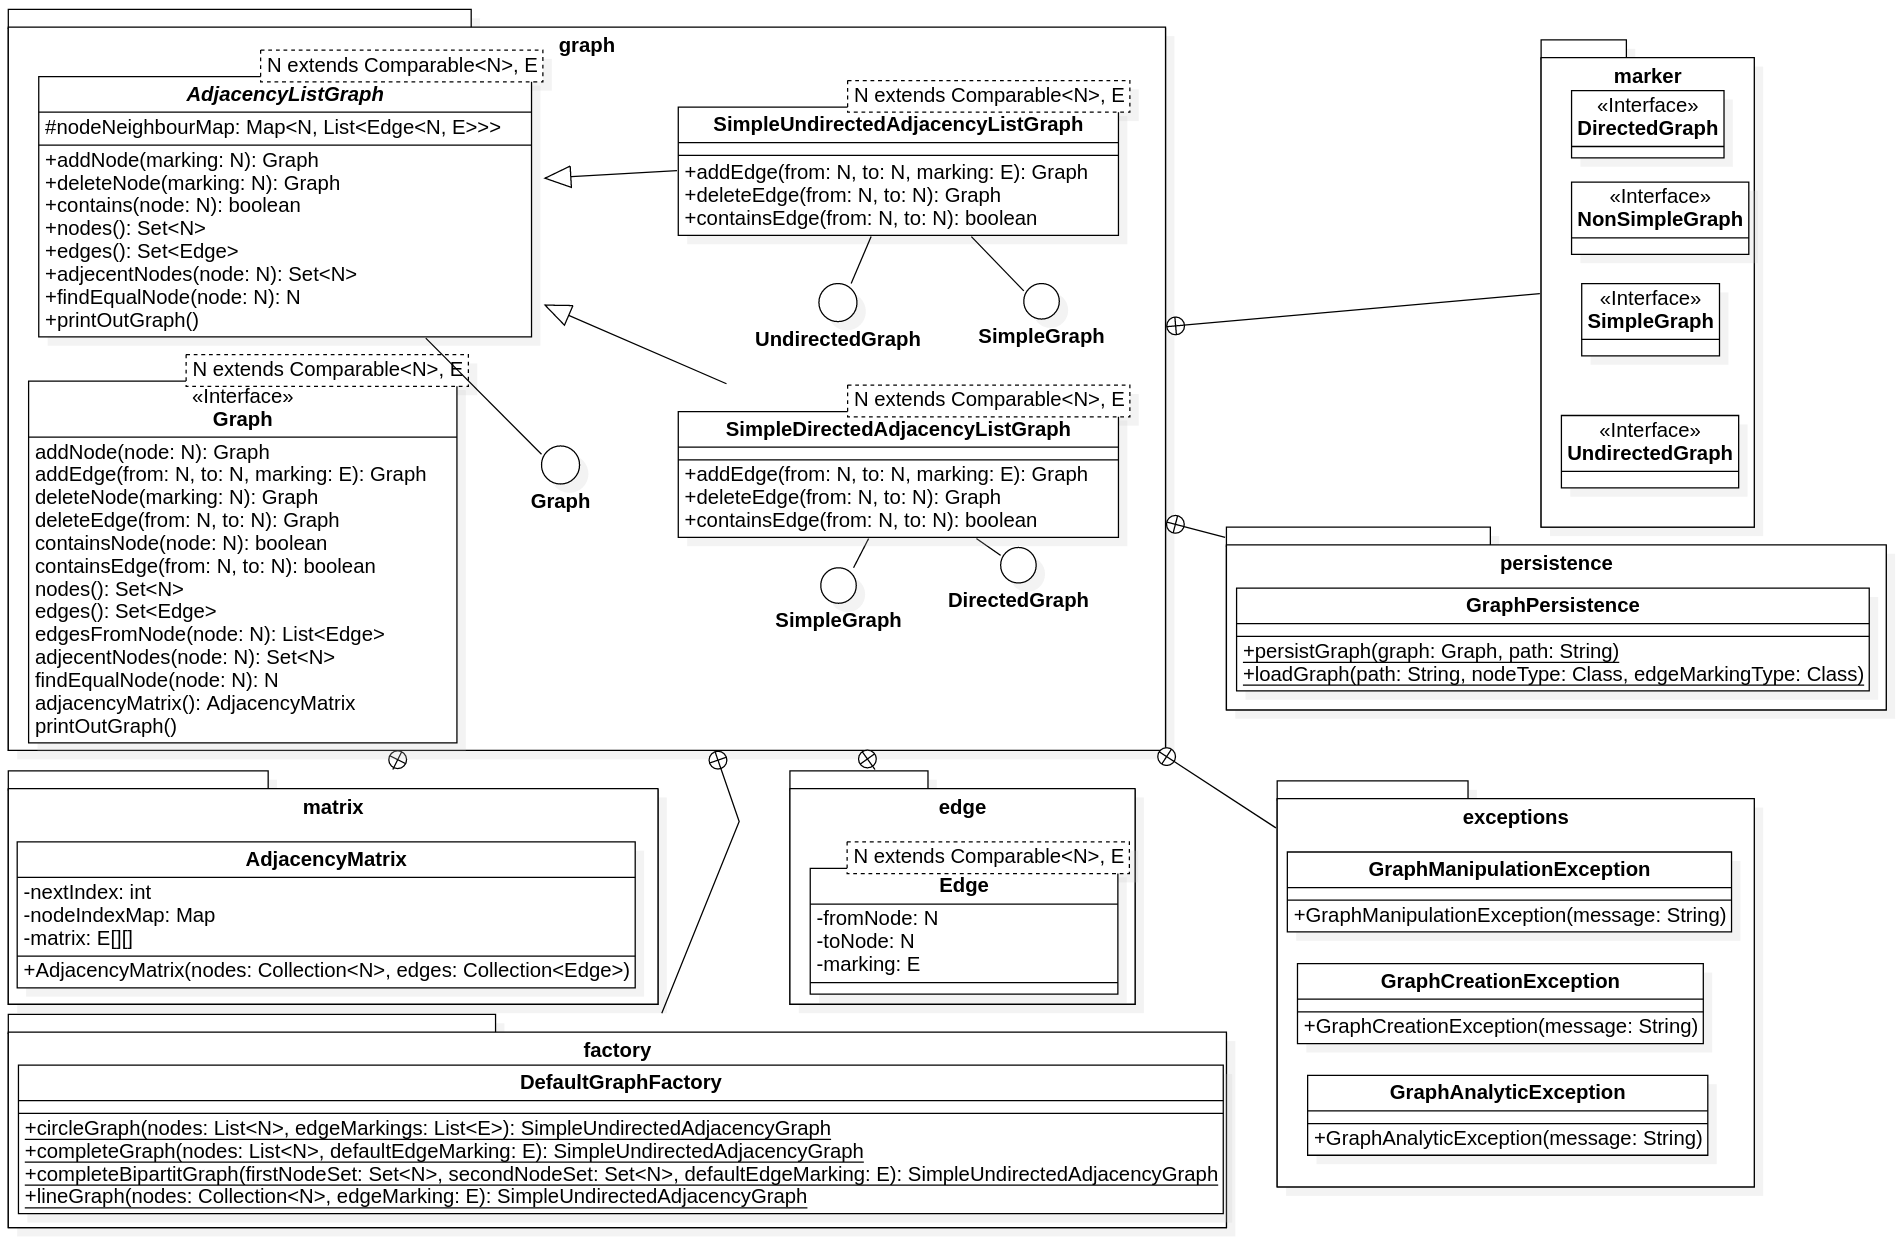
\includegraphics[scale=0.33]{Abbildungen/UML/graph_class_diagram.png}
		\caption[Klassendiagramm: Graphdatenstruktur]{Klassendiagramm: Graphdatenstruktur}
	\end{figure}
\end{landscape}
}
\subsubsection*{Metriken-Berechnung}
{
Durch die Bereitstellung einer Graph-Datenstruktur ist es nun möglich, eine Struktur bereitzustellen, die es ermögllicht alle gewünschten Metriken zu berechnen. Um die Berechung zu nutzen soll ein Mechanismus zur Verfügung gestellt werden, der den Zugriff auf die Kalkulation homogenisiert. D.h. es wird eine Schnittstellen-Klasse erzeugt, die sämtliche Berechnungsanfragen annimmt und an die Business-Logik weitergibt.

Zur Umsetzung dieses Mechanismus wird auf ein vereinfachtes Schichten-Muster zurückgegriffen \cite{balzert_lehrbuch_2011}. Die Klasse \textit{MetricsCalculation} stellt als eine Art Schnittstelle ("`bondary"') statische Methoden zur Berechung aller Metriken zur Verfügung. Es wird dabei zwischen drei Verschiedenen Metrik-Arten unterschieden.
\begin{myitemize}
	\item Graph-umfassende Metriken
	\item Knoten-beschreibende Metriken
	\item Metriken zur Beschreibung der Beziehung zwischen zwei Knoten
\end{myitemize}
Die jeweiligen Methoden nehmen den zu analysierenden Graphen und ggf. die zu untersuchenden Knoten entgegen. Zudem wird eine Instanz einer \textit{GraphMetric}, \textit{NodeMetric} oder \textit{NodeToNodeMetric} übergeben, die die zu berechnende Metrik identifiziert. Die aufgeführten "`Klassen"' sind Enumerationen, die jeweils die unterstützten Kennzahlen enthalten. Die Schnittstelltenfunktionen liefern dem Aufrufer schlussendlich eine Java-\textit{Number}, die sowohl Ganzzahlen als auch Gleitkommazahlen darstellen kann.

Nachdem die "`boundary"' die initiale Anfrage entgegennimmt, muss diese weiter verteilt werden. Genauer heißt das, dass die Anfrage an die jeweiligen Klassen weitergegeben wird, die die Berechung der eigentlichen Metrik übernehmen. Für diese Verteilung wird in der zweiten Schnicht ("`control"') die Klasse \textit{GraphMetricCalculationDistribution} genutzt, die je nach der gewählten Metrik, die korrekte Berechnungsklasse aufruft.

Die jeweiligen Berechnungsklassen enthalten ausschließlich statische Methoden, die eine Metrik für den Graphen berechnen und dabei logischerweise eine Zahl zurückgeben (Integer, Long oder Double). Diese Klassen sind dabei einmal nach den drei bereits bekannten Kategorien in Pakete sortiert und enthalten dann noch mal nur Metriken jeweils passend zu einer der in Kapitel 2 formulierten Kategorien. Da Metriken teilweise aufeinander aufbauen interagieren diese Klassen auch untereinander. Die jeweiligen Klassen heißen und berechnen:
\begin{myitemize}
	\item \textbf{BasicGraphMetricCalculation}: Berechnung grundlegender Graph-Metriken (Ordnung, Größe etc.)
	\item \textbf{DistanceGraphMetricCalculation}: Berechnung distanzbasierter Metriken (Radius und Durchmesser)
	\item \textbf{ChromaticNumberMetricCalculation}: Berechnung der chromatischen Zahl (exakt und mit Greedy-Algorithmus)
	\item \textbf{ChromaticIndexMetricCalculation}: Berechnung des chromatischen Indexes (exakt und mit Greedy-Algorithmus)
	\item \textbf{DensityMetricCalculation}: Berechnung der Graph-Dichte
	\item \textbf{BasicNodeMetricCalculation}: Berechnung grundlegender Metriken für einen Knoten (z.B. Grad)
	\item \textbf{DistanceNodeMetricCalculation}: Berechnung der Extrenzität eines Knoten
	\item \textbf{CentralityMetricCalculation}: Berechnung der aufgeführten Zentralitätsmetriken
	\item \textbf{NodeToNodeDistanceMetricCalculation}: Berechnung der Distanz zwischen zwei Knoten innerhalb eines Graphen
\end{myitemize}
Weiterhin benötigen einige Metriken bestimmte Hilfsobjekte und -algorithmen, damit sie berechnet werden können. Hierzu zählen ein generisches Tupel-Objekt und Algorithmen zur Berechnung des Binomialkoeffizienten und der Breiten- und Tiefensuche. Zudem werden weitere Hilfsmethoden zur Verfügung gestellt zum Füllen und klonen von Java-Maps und zum invertierten von Graphen. Beim invertieren werden werden alle Kanten zu Knoten und die neuen Knoten sind adjazent zueinander, wenn die ursprünglichen Kanten inzident zueinander waren. Dies ist wichtig zur Berechnung des chromatischen Index.

Aus statischer Sicht sind keine weiteren Klassen notwendig, um die Berechung der Graphmetriken zu gewährleisten. Einzig gibt es noch zwei weitere Exceptions, die hinzugefügt werden. Die \textit{MetricChoiceException} wird geworfen, falls die Berechnung einer Metrik stattfindet, die nicht implementiert ist. Die \textit{MetricCalculationException} wird dann verwendet, falls bei der Berechnung einer Metrik ein Fehler auftritt. Beispielsweise ist das der Fall, falls ein für einen Graph die Größte berechnet werden soll, der aber nicht als gerichtet oder ungerichtet markiert wurde.

Wie an der Beschreibung gesehen werden konnte, sind die Methoden für die Metrikenberechnung alle ausschließlich statisch. Das entspricht zwar nicht dem Paradigma der Objektorientierung, ist allerdings vorteilhaft, da so nicht unnötigerweise attributlose Berechnungsobjekte erstellt werden müssen. Außerdem drückt dies auch den funktionalen Charakter der Bibliothek aus. Die jeweiligen Methoden zur Berechnungen der Kennzahlen lösen keine Seiteneffekte aus und liefern so bei gleichem Input den gleichen Output. Dies ähnelt dem funkionalen Programmierparadigma, was die statischen Methoden imitieren. \cite{chiusano_functional_2015}

Die beschriebenen Klassen können nun auch wieder in einem Klassendiagramm aufgezeigt werden, dass in Abbildung 3.3 zu sehen ist.
\begin{figure}[htp]
	\centering
	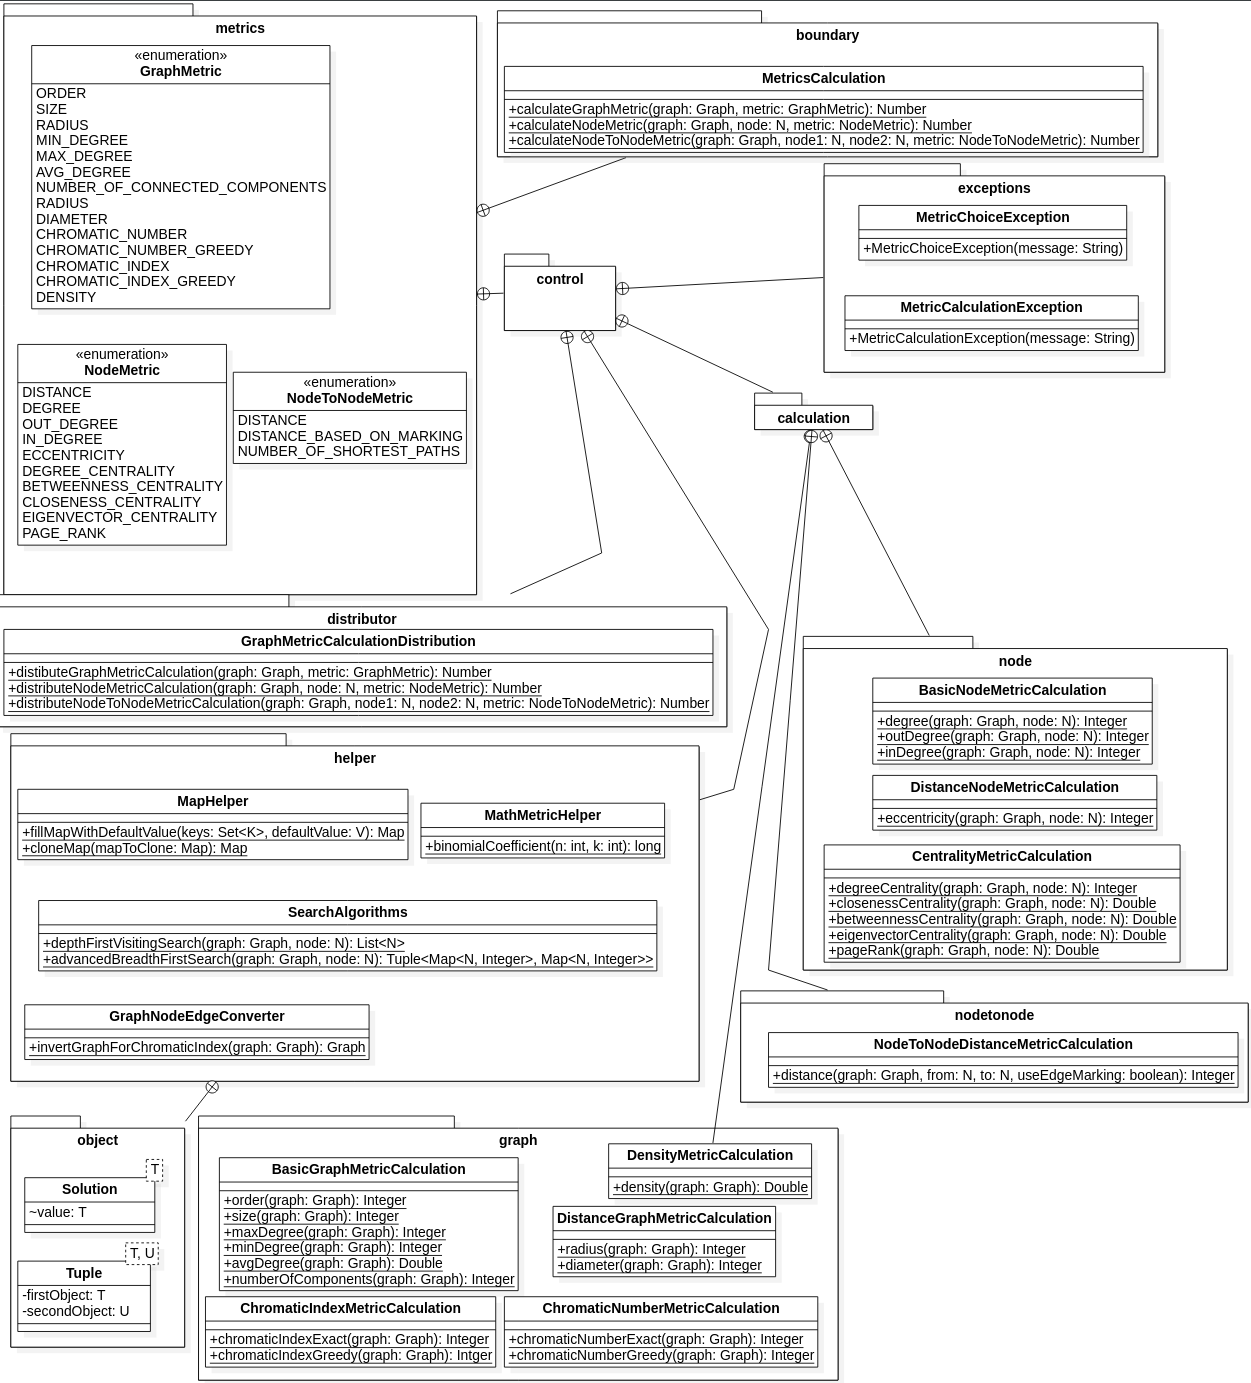
\includegraphics[scale=.38]{Abbildungen/UML/metrics_class_diagram.png}
	\caption[Klassendiagramm: Metriken-Berechnung]{Klassendiagramm: Metriken-Berechnung}
\end{figure}
}
\subsection{Dynamische Aspekte}
{
Dadurch, dass die Statik der Klassenbibliothek nun feststeht und durch diese die formulierten funktionalen Anforderungen gedeckt sind, soll noch auf den dynamischen Entwurfsaspekt der Bibliothek eingegangen werden. Konkret soll erläutert werden, wie eine Metriken-Berechnung von Statten geht.

Zur Beschreibung soll als Beispiel die Berechnung der Closeness Centrality herhalten. Die Berechnung der anderen Metriken erfolgt analog, bzw. ähnlich. Bevor aber eine Metrik berechnet werden kann, ist es nötig einen Graphen zu erstellen und zu manipulierten bzw. zu füllen. Im Rahmen des Beispiels soll ein simpler, ungerichteter Adjazenzlistengraph erstellt werden, der als Knoten und Kantenmarkierung Ganzzahlen entgegennimmt. Hierfür lässt sich einer der bereits implementierten Graphen der Bibliothek verwenden. Der Graph selbst wird in einer Variable gespeichert, die den Typ \textit{Graph} hat. Damit ist der Graph nur über die definierte Schnittstelle zu manipulieren und kann für die Metrikenberechnung genutzt werden. Anschließend an die Erstellung können Knoten und Kanten eingefügt werden. Im Beispiel sollen die zwei Knoten 1 und 2 hinzugefügt werden. Zudem wird eine Kante zwischen beiden erstellt, die mit 1 markiert ist. Wie das im Rahmen eines Sequenzdiagramms aussieht, zeigt Abbildung 3.4.
\begin{figure}[ht!]
	\centering
	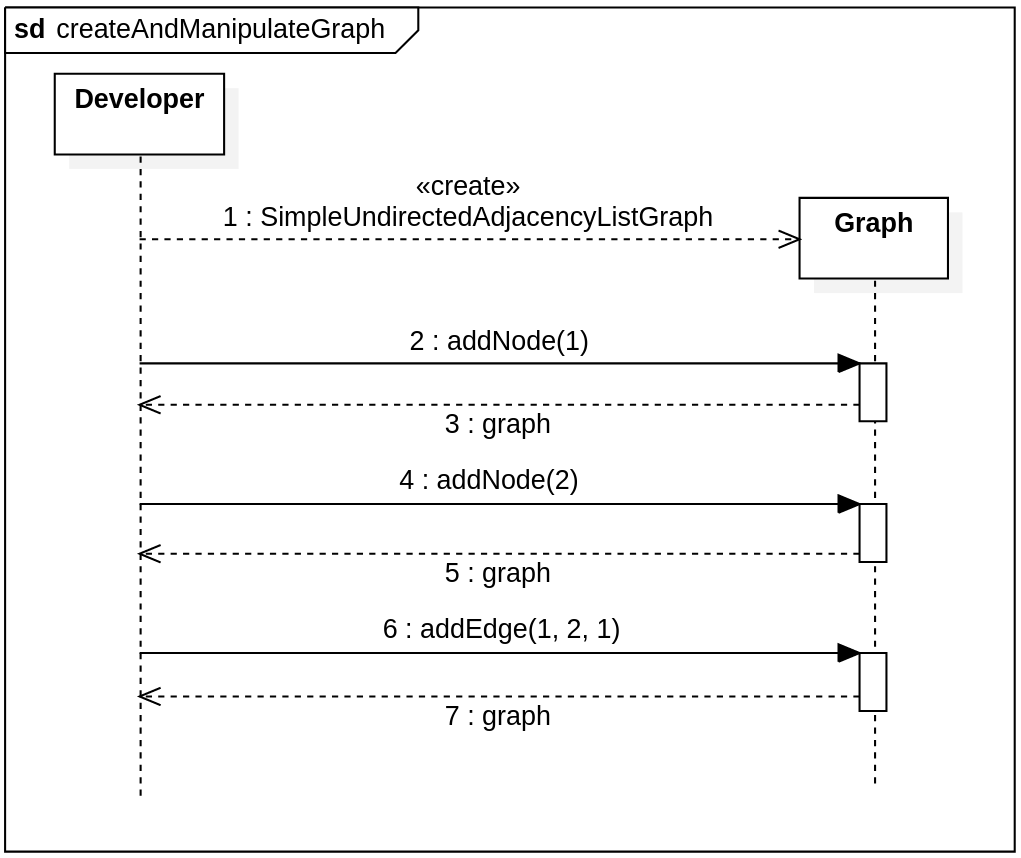
\includegraphics[scale=.38]{Abbildungen/UML/sequence_graph_creation.png}
	\caption[Sequenzdiagramm: Grapherstellung und- manipulation]{Sequenzdiagramm: Grapherstellung und- manipulation}
\end{figure}
Nachdem der Graph erstellt wurde, können auf ihm alle Metriken berechnet werden. In diesem Fall übergibt der Entwickler den Graph mit den sonstigen Argumenten der \textit{MetricCalculation}, die wiederum die Anfrage an die weiter unten liegende Schicht weitergibt. Hier verteilt die \textit{GraphMetricCalculationDistribution} die Anfrage an die korrekte Berechnungsklasse. Im Fall der Closeness Centrality ist das die Klasse \textit{CentralityMetricCalculation}. Diese kann die Metrik allerdings nicht alleine berechnen und benötigt die Hilfe eines Suchalgorithmus (Breitensuche). Infolgedessen ruft die Klasse die \textit{SearchAlgorithms}-Klasse auf und kann mit deren Ergebnis die Metrik berechnen und schlussendlich den höheren Schichten zurückgeben. Abbildung 3.5 zeigt die dynamische Folge der Metriken-Berechnung für die Closeness Centrality in einem Sequenzdiagramm.
\begin{figure}[ht!]
	\centering
	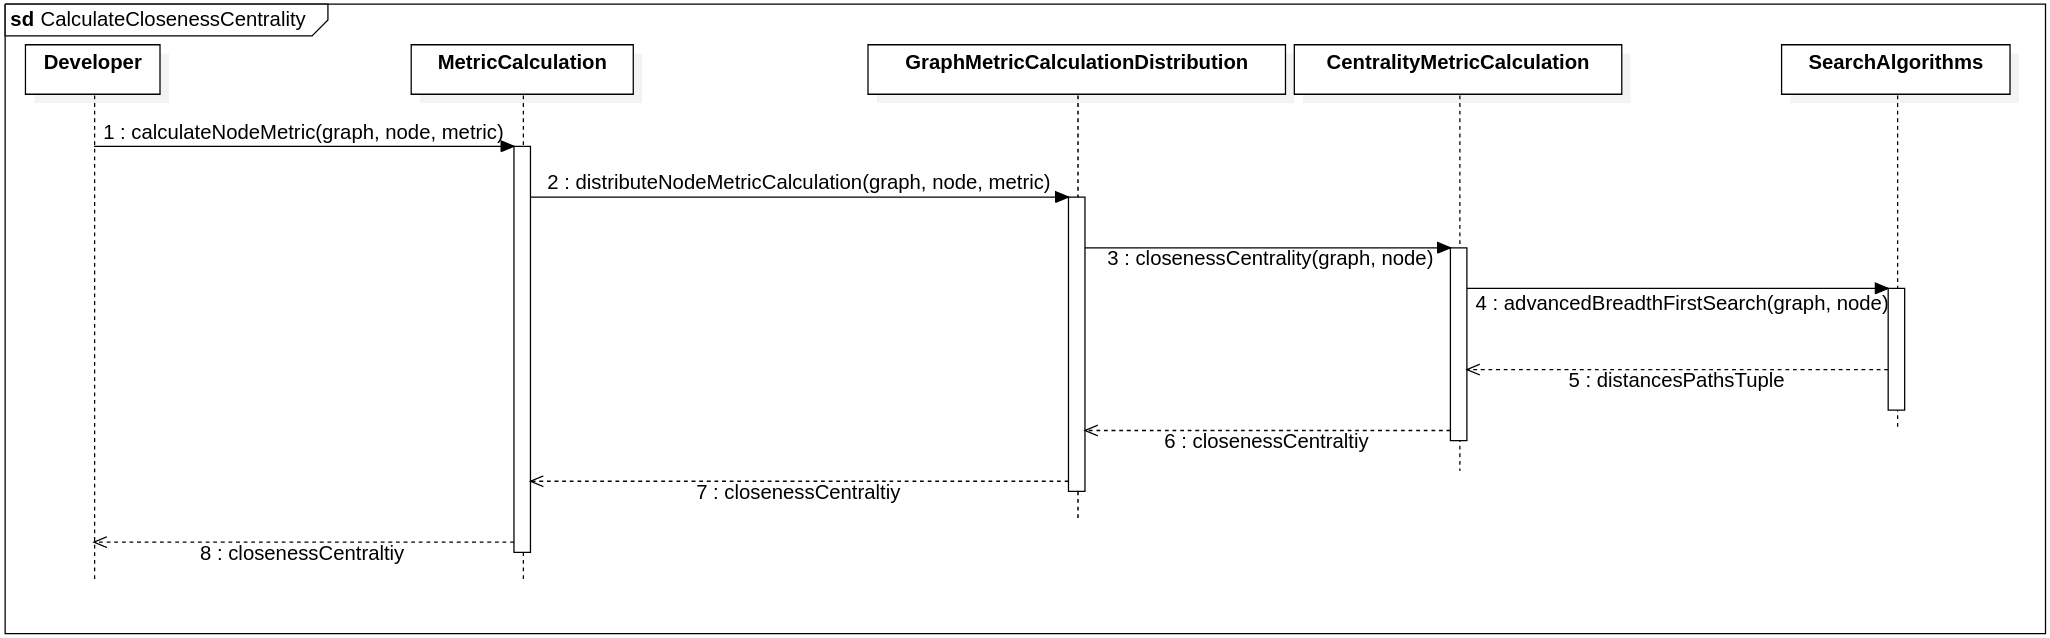
\includegraphics[scale=.22]{Abbildungen/UML/sequence_metric_calc.png}
	\caption[Sequenzdiagramm: Metriken-Berechnung (Closeness Centrality)]{Sequenzdiagramm: Metriken-Berechnung (Closeness Centrality)}
\end{figure}
}
\section{Algorithmik und Implementierung der Graph-Metriken}
{
Nachdem die Beschaffenheit und grundsätzliche Funktionsweise der Klassenbibliothek erläutert wurde, soll nun noch darauf eingegangen werden, wie die jeweiligen Metriken berechnet werden. Vor allem ist es interessant die Algorithmik einzelner Metirken zu beleuchten. Es werden dabei alle implementierten Metriken betrachtet. Zuerst werden die Graph-übergreifenden, dann die Knoten-beschreibenden und abschließend die Distanz zwischen zwei Knoten beschrieben.
}
\subsubsection*{Graph-umfassende Metriken}
{
Zu den Graph-umfassenden Metriken gehören zunächst die vorgestellten grundlegenden Metriken (siehe. 2.1), die für einen ganzen Graph gehören. Diese sind meist auch recht einfach zu berechnen. Für die Ordnung eines Graphen wird abgefragt, wie groß die Menge der Knoten ist. Die Knotenmenge kann dabei mit dem Aufruf \textit{graph.nodes()} erfragt werden, der im Graph-Interface definiert ist. Ähnlich verhält es sich auch bei der Größe des Graphen, wobei hier die Kantenmenge abgerufen wird (\textit{graph.edges()}). Eine Besonderheit besteht hierbei noch in der Unterscheidung zwischen gerichteten und ungerichteten Graphen. Ist der Graph nämlich ungerichtet so wird seine Größe durch Zwei geteilt. Dies wird durch den \textit{instanceof}-Aufruf von Java und die Marker-Interfaces erreicht.

Zur Berechnung von Minimal-, Maximal- und Durchschnittsgrad bedient sich die Bibliothek der Stream-API von Java. Diese API ermöglicht es u.a. mithilfe von Lambda-Ausdrücken Datenmengen in Java zu filtern, abzubilden, zu reduzieren und zu sammeln. \cite{ullenboom_java_2014} Zur Berechnung werden die Knoten des Graphen in einem Stream verarbeitet und auf ihren jeweiligen Grad abgebildet. Hierfür wird die Grad-Metrik der Bibliothek genutzt. Auf den anschließenden Ganzzahl-Stream kann eine \textit{min()-, max()-} oder \textit{average()}-Anfrage aufgeführt werden. Da die API hierbei einen Java \textit{Optional} zurückgibt, muss dieser noch aufgelöst werden, indem bei Nichtvorhandensein eines Ergebnisses eine \textit{MetricCalculationException} geworfen wird. Dies ist beispielsweise der Fall, wenn der Graph leer ist. Der gesamte Aufruf zur Berechnung der Metrik sieht dann folgendermaßen aus (Beispiel für Maximalgrad):
\begin{lstlisting}
	return graph.nodes().stream().mapToInt(node ->
				BasicNodeMetricCalculation.degree(graph, node)).max()
				.orElseThrow(() -> new MetricCalculationException(MESSAGE));
\end{lstlisting}
Für die Berechnung der Anzahl der Zusammenhangskomponenten wird sich dem Algorithmus bedient, der bereits in 2.1 beschreiben wurde. D.h. wird eine Tiefensuche für alle Knoten initiiert, falls diese nicht bereits von einer anderen Tiefensuche besucht wurden. Hierfür gibt der Tiefensuche-Algorithmus immer die Menge an Besuchten Knoten zurück. Die Tiefensuche selbst ist Teil der Helfermethoden und bedient sich eines Stapels zur Koordinierung der Suche. Zu Beginn der Algorithmus wird eine List für die besuchten Knoten und ein Stapel initialisiert. Der Start-Knoten wird in beide Kollektionen eingefügt. Anschließend wird solange ein Knoten vom Stapel genommen und seine nicht besuchten Nachbarn in die Kollektionen gelegt, bis der Stapel final leer ist. Danach wird Liste der besuchten Knoten zurückgegeben.

Nach grundlegenden, graph-übergreifenden Metriken soll erklärt werden, wie das einzige Dichtemaß des Bibliothek berechnet wird. Die Dichte eines Graphen wurde in 2.4 beschrieben und kann genauso berechet werden, wie die Formel im Kapitel es vorschreibt. So wird einfach die Größe des Graphen durch den Binomialkoeffizienten \(|V|\) über \(2\) geteilt und das Ergebnis zurückgegeben. Hervorzuheben ist, dass beim Berechnen sowohl geprüft wird, ob ein simpler Graph vorliegt und ob der Graph gerichtet ist oder nicht. Der Graph muss simpel sein, da die Berechnung nur möglich ist, wenn keine Schlingen und Doppelkanten im Graph möglich sind. Weiterhin ist es relevant ob der Graph gerichtet ist oder nicht, da bei einem nicht gerichteten Graph der Binomialkoeffizienten verdoppelt werden muss, da der Graph ja potenziell doppelt so viele Kanten tragen kann. Zur Berechnung des Binomialkoeffizienten wird sich eines effizienten iterativen Algorithmus bedient, der die Produktformel für den Binomialkoeffizienten implementiert, die folgendermaßen lautet:
\[
	\binom{n}{k}=\prod_{i=1}^{k}\frac{n+1-i}{i}
\]
Die Implementierung dieser Produktformel, kann innerhalb von Java folgendermaßen aussehen. Hierbei wird zuerst abgefangen, falls \(k\) Null ist. Ist dies der Fall, ist das Ergebnis immer 0. Ist wiederum \(2 * k\) größer als \(n\), so wird \(k\) zu \(n - k\). Dies ist möglich, da das Pascal'sche Dreieck, in dem die Werte des Binomialkoeffizienten stehen, symmetrisch ist und \(k\) die Spalten in diesem Dreieck rerpäsentiert. Zudem verkürzt das verkleinerte \(k\) die Zählschleife und somit dem Algorithmus.
\begin{lstlisting}
	if (k == 0) return 1L;
	if (2 * k > n) k = n - k;
	long solution = 1L;
	for (int i = 1; i <= k; i++) {
		solution = solution * (n + 1 - i) / i;
	}
return solution;
\end{lstlisting}
Für die distanzbasierten, graph-übergreifenden Metriken wird sich wieder der Java Stream-API bedient. Sowohl für den Radius als auch für den Durchmesser wird die Extrenzität aller Knoten benötigt. Ähnlich wie beim Maximal- oder Minimalgrad werden alle Knotens des Graphen auf eine Granzzahl abgebildet. In diesem Fall auf die Extrenzität. Dann kann wieder über die \textit{max()} (Durchmesser) und \textit{min()} (Radius) die jeweilige Metrik extrahiert werden. Auch hier gilt, dass bei einem leeren Graphen über die \textit{Optional}-Logik eine \textit{MetricCalculationException} geworfen wird.

Die letzten graph-übergreifenden Metriken, die umgesetzt wurden, sind die chromatische Zahl und der chromatische Index. Zur Berechnung der chromatischen Zahl wurden zwei Algorithmen implementiert. Eine exakte Berechnung des NP-vollständigen Problems und die bereits vorgestellte Greedy-Variante. Die Greedy-Variante konnte so umgesetzt werden, wie sie in 2.6 beschreiben wurde. Um für den Algorithmus die jeweilige niedrigst mögliche Farbe zu wählen, werden jeweils die zum Knoten adjazenten Knotenfarben in eine Liste geladen und anschließend, beginnend mit der niedrigsten Farbe, durch die Farben iteriert und geprüft, ob die Farbe in der Liste ist. Ist sie das nicht, kann sie als Farbe für den Knoten verwendet werden. Die Ermittlung der exakten chromatischen Zahl erwies sich als schwieriger. Um über alle möglichen Färbungen zu iterieren, wie das bei der exakten Berechnung nötig ist, müssen jeweils \(n\) Zählschleifen ineinander geschachtelt werden, die jeweils bis zur maximal höchsten Färbung zählen und dies ihrem korrespondierenden Knoten zuweisen. Sowohl \(n\) als auch die höchst mögliche Farbe entspricht der Ordnung des Graphen. Um diese beliebige Schachtelung der Zählschleifen zu erreichen, muss ein rekursiver Algorithmus entworfen werden. Um den rekursiven Abstieg zu koordinieren, wird eine Level-Variable eingefügt, die anfangs so groß ist, wie die Ordnung des Graphen. Bei jedem Abstieg wird diese um eins reduziert und sie markiert, welcher Knoten bei welchem Aufruf zu Färben ist. Ist das Level gleich 0, tritt der Basis-Fall der Rekursion ein und es wird geprüft, ob die jeweilige aktuelle Färbung legal ist. Fall diese das ist, wird geprüft, wie viele verschiedene Farben genutzt wurden und in ein einheitliches Lösungsobjekt die aktuell kleiste legale Färbungszahl geschrieben. Das Lösungsobjekt, das dem Algorithmus übergeben wird, kann anschließend ausgelesen werden. Um zu prüfen, ob eine Färbung legal, wird über alle Knoten iteriert und geprüft, ob einer der Nachbarn jeweils die gleiche Farbe hat wie der aktuelle Knoten. Ist dies nur einmal der Fall, so ist die Färung nicht legal. Im Pseudocode ausformuliert, sieht der Algorithmus folgendermaßen aus:
\begin{lstlisting}
	chromaticNumberExact(graph, nodeColorings: List<[Node, Integer]>, level, maxColor, solution) {
		if (level == 0) { // Basisfall
			if (isLegalColoring(graph, nodeColorings)) {
				solution = Math.min(solution, colorNumber(nodeColorings));
			}
		} else { // Rekursionsfall
			for (int i = 1; i <= maxColor; i++) {
				nodeColorings.get(level).setColor(i);
				chromaticNumberExact(graph, nodeColorings, level - 1, maxColor,
				solution);
			}
		}
	}
\end{lstlisting}
Bereits beim statischen Entwurf der Bibliothek wurde gezeigt, wie die Berechnung des chromatischen Index erfolgt. Hierfür wird der Code der chromatischen Zahl einfach wiederverwandt. Auch beim chromatischen Index wird eine exakte und eine Greedy-Variante bereitgestellt. Grundsätzlich wird der Graph zur Berechnung also invertiert und anschließend die schon beschriebenen Algorithmen angewandt. Bei der Invertierung wird jede Kante in einen Knoten umgewandelt und anschließend dort Kanten eingefügt, falls beim ursprünglichen Graph zwei Kanten inzident zueinander waren.
}
\subsubsection*{Knoten-beschreibende Metriken}
{
Auch bei den Knoten-beschreibenden Metriken gibt es bestimmte grundlegende Metriken. Der Ausgangsgrad eines Knotens wird dabei berechnet, indem die Größe der Menge seiner adjazenten Knoten (\textit{graph.adjacentNodes(node)}) zurückgegeben wird. Zur Berechnung des Eingangsgrads wird die Liste aller Kanten (\textit{edges()}) gefiltert und dabei geschaut, ob der Knoten, zu der die Kante zeigt, gleich dem zu untersuchenden Knotens ist. Für den Eingangsgrad kann dann diese gefilterte Liste gezählt werden. Bei der Berechnung des allgemeinen Knotengrades muss wieder unterschieden werden, ob ein gerichteter Graph vorhanden ist. Ist er ungerichtet so kann als Graph einfach der Ausgangsgrad genutzt werden. Ist er gerichtet, müssen sowohl ein- als auch ausgehende Kanten einzeln gezählt werden. Dies wird erreicht durch die Addition des Ausgangs- und Eingangsgrads.

Um die Extrenzität, die auch für den Durchmesser und den Radius gebraucht wird, eines Knoten zu berechnen, werden wieder alle Knoten des Graphen auf eine Granzzahl abgebildet. Die entstehenden Ganzzahlen sind die Distanzen zwischen dem zu Untersuchenden Knoten und allen anderen Knoten. Aus der so entstanden Distanzliste kann dann die höchste Zahl entnommen werden, die wiederum die Extrenzität des Knotens darstellt.

Die Metrikenklasse mit den meisten Implementierungen bei den Knoten-beschreibenden Metriken sind die Zentralitätsmetriken. Die erste Zentralitätsmetrik ist die Degree Centrality. Diese ist äußerst einfach zu berechnen, da sie deckungsgleich zum Grad des Knotens ist. D.h. die Aufgabe wird einfach an die Grad-Berechnung deligiert, damit kein doppelter Code geschrieben werden muss.

Die erste komplexere Centrality-Berechnung ist die der Closeness Centrality. Für diese Metrik muss man wissen, wie weiter der zu untersuchende Knoten von allen anderen Knoten entfernt ist. Um diese Distanzen herauszufinden, wird sich einer Breitensuche bedient, die eine Map zurückliefert, die die anderen Knoten auf ihre Distanz vom Ausgangsknoten abbildet. Die Breitensuche wird genauer in einem weiteren Abschnitt beschrieben. Sind zunächt die Distanzen vorhanden, können diese einfach aufsummiert werden, um anschließend, die Formel für die Closeness Centrality anzuwenden. Ist die aufsummierte Distanz, wird als Ergebnis die höchstmögliche Ganzzahl zurückgegeben, um \(\infty\) zu repräsentieren.

Um die Betweenness Centrality zu berechnen, ist es nötig die Funktionen \(\sigma_{st}(v)\) und \(\sigma_{st}\) zu implementieren. Da die Funktion \(\sigma_{st}(v)\) auf \(\sigma_{st}\) basiert, muss voralledem die zweitere algorithmisch umgesetzt werden. Auch hierbei hilft die Breitensuche. Da \(\sigma_{st}\) die Anzahl der kürzesten Wege zwischen zwei Knoten darstellt und damit eine Metrik für sich ist, wird diese später noch genauer beschrieben. Ist \(\sigma_{st}\) umgesetzt, kann \(\sigma_{st}(v)\) einfach so im Programm umgesetzt werden, wie in Kapitel 2.5 beschrieben. Hierbei wird für die Berechnung der Distanzen zwischen zwei Knoten auf die korrespondierende Implementierte Metrik zugegriffen, die noch genauer erläutert wird. Mit den beiden implementierten Funktionen kann die Betweenness Centrality einfach über zwei Zählschleifen umgesetzt werden. Die jeweiligen Schleifen iterieren über alle Knoten des Graphen. Falls die beiden betrachteten aktuellen Knoten \(s\) und \(t\) nicht dem zu untersuchenden Knoten entsprechen und \(s\) und \(t\) nicht gleich sind, kann zur Betweenness Centrality des Knotens ein Summand addiert werden. Hierbei ist der Summand einfach die Anzahl \(\sigma_{st}(v)\) durch \(\sigma_{st}\) geteilt, wie es die Formel auch vorgibt. Ist die Iteration vorbei kann das Ergebnis der Betweenness Centrality zurückgegeben werden.

Eine weitere Zentralitätsmetrik ist die Eigenvector Centrality. Diese wird in der Klassenbibliothek mittels des vorgestellten Power Iteration-Algorithmus berechnet. Da dieser Algoritmus mittels Matrixmultiplikation verläuft benötigt es zwei Dinge. Zuerst muss für den Graph eine Repräsentation mittels einer Adjazenzmatrix bereitgestellt werden. Zweitens muss eine Funktion zur Matrixmultiplikation vorhanden sein. Für ersteres dient die Methode \textit{adjacencyMatrix()} des \textit{Graph}-Interfaces. Die im \textit{AdjacencyMatrix}-Objekt enthaltene Matrix wird anschließend so umgewandelt, dass statt der Kantenmarkierung eine 1 oder 0 in den Matrixpositionen steht. Eine 1 steht im Eintrag, falls dort vorher auch eine Kante eingetragen war. Ansonsten wird eine 0 eingetragen. Für die Matrixmultiplikation wird mittels Maven die "`Apache Commons"'-Bibliothek eingebunden, da diese eine effiziente Implementierung für die Matrixmultiplikation bietet. Neben der Adjazenzmatrix muss für die Poweriteration auch der Startvektor erstellt werden, der so viele Zeilen wie die Adjazenzmatrix hat und eine Spalte hat, wobei jeder Eintrag 1 ist. Die Power Iteration selbst ist ein rekursiver Algorithmus. In diesem wird zunächst ein neuer Ergebnisvektor berechnet, indem die Adjazenzmatrix mit dem aktuellen Eigenvector Centrality-Vector multipliziert wird. Zu Anfang ist das der erstellte Startvektor. Der so entstehende neue Vektor wird normalisiert und der Normalisierungswert wird zusätzlich gespeichert. Der Basisfall der Rekursion tritt nun auf, wenn die Berechnung konvergiert. Dies ist der Fall, wenn der aktuelle Normalisierungswert fast gleich dem alten Normalisierungswert ist (maximale Differenz 0,001). Dann kann der Ergebnisvektor mit den Eigenvector Centralities zurückgegeben werden und der Wert für den zu untersuchenden Knoten herausgenommen werden. Konvergiert die Berechung nicht, tritt der Rekursionsfall ein. Hierbei wird einfach die Power Iteration mit dem neuen Eigenvector Centrality-Vektor erneut aufgerufen. Zudem wird der vorher berechnete Normalisierungswert mitgegeben, um zu prüfen, ob die Berechnung konvergiert. Als Pseudocode kann der Algorithmus folgendermaßen zusammengefasst werden:
\begin{lstlisting}
	double[][] powerIteration(adjacencyMatrix, vector, normalizedValue) {
		newVector = adjacencyMatrix * vector;
		newNormalizedValue = calcNormalizedValue(newVector);
		normalizeVector(newVector, newNormalizedValue);
		if (powerIterationConverged(normalizedValue, newNormalizedValue)) {
			return newVector;
		} else {
			return powerIteration(adjacencyMatrix, newVector,
				newNormalizedValue);
		}
	}
\end{lstlisting}
Die letzte Zentralitätsmetrik, die umgesetzt wurde, ist der Page Rank. Auch hier wird ein Rekursiver Algoritmus zur Berechnung genutzt. Zu Beginn bekommt jeder Knoten innerhalb einer Java-Map den Page Rank \(1/|V|\) zugewiesen. Anschließend kann der eigentliche Algorithmus gestartet werden. Da dieser auch terminiert, wenn die Werte in der Map gegen einen bestimmten Wert konvergieren, wird im ersten Schritt die Map kopiert. Schlussendlich kann die in 2.5 vorgestellte Formel für den Page Rank angewandt werden. Hierfür wird über alle Knoten des Graphen iteriert und die Formel angewandt und anschließend der neue Wert in der Map für den Knoten gespeichert. Sind alle Werte sehr ähnlich zur Map aus vorigen Funktionsaufruf (Differenz < 0.001), so tritt der Basisfall ein und der Algorithmus terminiert und aus der Map kann der Page Rank aller Knoten abgelesen werden. Ansonsten tritt der Rekursionsfall ein und der Page Rank-Algorithmus wird erneut mit der neuen Map aufgerufen. Im Pseudocode sieht das folgendermaßen aus. Der der Dämpfungsfaktor, der für den Algorithmus gewählt werden muss, steht als Konstante in der Klasse zur Verfügung und beträgt 0,85.
\begin{lstlisting}
	Map<Node, Double> pageRank(graph, previousMap, pageRankMap) {
		newPageRankMap = clone(pageRankMap);
		for (node : graph.nodes()) {
			newPageRank = 1 - MODERATION_FACTOR;
			pageRankAddend = 0;
			for (adjacentNode: graph.adjacentNodes(node)) {
				pageRankAddend += previousMap.get(adjacentNode) /
					outDegree(graph, adjacentNode);
			}
			pageRankAddend *= MODERATION_FACTOR;
			newPageRankMap.put(node, newPageRank + pageRankAddend);
		}
		if (pageRankConverges(previousMap, newPageRankMap)) {
			return newPageRankMap;
		} else {
			return pageRank(graph, pageRankMap, newPageRankMap);
		}
	}
\end{lstlisting}
}
\subsubsection*{Metriken zwischen zwei Knoten}
{
Die erste Metrik, die die Klassenbibliothek zwischen zwei Knoten definiert, ist die kürzeste Distanz zwischen diesen. Zur Berechung dieser haben sich einige Algorithmen verausgebildet. So können z.B. eine Breitensuche, der Djikstra-Algorithmus oder der A*-Algortihmus das Problem korrekt lösen. Bei der Breitensuche muss allerdings die Distanz zwischen zwei Knoten immer 1 sein und der A*-Algorithmus benötigt eine Heuristik, um effizient zu arbeiten. Im Rahmen dieser Bibliothek wurde zur Berechnung der Distanz die "`Uniform Cost Search"' gewählt, wie sie im Buch "`Artificial Intelligence - A modern approach"' von Stuart Russell und Peter Norvig beschrieben ist. Zu Beginn des Algrithmus wird zunächst eine Vorrangwarteschlange initialisiert, die immer den Knoten an vorderste Stelle stellt, der die niedrigste Distanz zum Ausgangsknoten hat. Zudem wird eine Liste der besuchten Knoten angelegt. Anfangs wird in diese Warteschlange der Ausgangsknoten mit Distanz 0 gelegt. Anschließend wird das erste Element aus der Warteschlange genommen und geprüft, ob dies der Zielknoten ist. Wenn ja, kann seine hinterlegte Distanz zurückgegeben werden. Falls nicht, wird der Knoten in die Liste der besuchten Knoten hinzugefügt und in die Vorrangwarteschlange werden alle seine noch nicht besuchten Nachbarknoten gelegt. Diese bekommen die Distanzmarkierung \textit{Markierung aktueller Knoten + Distanz zu jeweiligen Nachbar}. Dieser Vorgang wird solange wiederholt, bis die Warteschlange leer ist. Falls dies eintrifft und somit kein Weg zwischen den Knoten gefunden wurde, gibt der Algorithmus den maximalen Ganzahlwert des Typs \textit{Integer} zurück, um die Distanz \(\infty\) zu repräsentieren. Der implementierte Algorithmus kann sowohl mit Kantenmarkierungen für die Distanz arbeiten oder für jede Kante die Distanz 1 annehmen. Falls die Kantenmarkierung berücksichtig werden soll, muss dies bei Aufruf angegeben werden und die Kantenmarkierung muss zu einer Zahl castbar sein. \cite{russell_artificial_2016}

Die letzte Metrik deren Implementierung beschreiben wird, ist eine spezielle Metrik, die deswegen implementiert wurde, da sie für die Betweenness Centrality gebraucht wird. Damit die Anzahl der kürzesten Wege zwischen zwei Knoten berechnet werden kann, wird sich wie beschrieben einer speziellen Breitensuche bedient. Die gleiche Breitensuche wird auch für die Distanzen bei der Closeness Centrality genutzt. Für beide Nutzungsszenarien liefert die implementierte Breitensuche ein Ergebnis vom Typ \textit{Tuple\textless Map\textless N, Integer\textgreater , Map\textless N, Integer\textgreater\textgreater}. In der ersten Map werden alle erreichbaren Knoten gelistet und auf ihre Distanz vom Ausgangsknoten abgebildet. In der zweiten Map sind die gleichen Knoten verzeichet und werden auf die Anzahl der kürzesten Wege vom Ausgangsknoten aus abgebildet. Somit kann das Ergebnis für die Berechnung der Anzahl der kürzesten Wege zwischen zwei Knoten einfach aus der zweiten Map gelesen werden. Die verwendete spezialisierte Breitensuche wurde von Said Sryheni in seinem Artikel "`Number of Shortest Paths in a Graph"' beschrieben \cite{sryheni_number_2020}. Die Suche verfolgt dabei grundsätzlich das gleiche Prinzip wie die beschriebene Tiefensuche, nur dass anstatt eines Stapels eine Warteschlange als Hilfsstruktur gewählt wird. Aus der Warteschlange wird zunächst der erste Knoten entnommen und dann über all seine Nachbarn iteriert. Ist ein Nachbar noch nicht besucht, wird er in die Warteschlange eingereit und als besucht markiert. Zusätzlich wird nun geprüft, ob die akutelle Distanz zum jeweiligen adjazenten Knoten kleiner ist, als die eingetragene. Ist dies der Fall wird die nun kleinere gefundene Distanz eingetragen. Zudem kann die Anzahl der gefunden kürzesten Wege zum Knoten auf die Anzahl der kürzesten Wege gesetzt werden, die der aktuell betrachtete Knoten hat. Ist dies nicht der Fall wird geprüft, ob die neu gefundene Distanz gleich zu der bereits eingetragenen ist. Fall dies zutrifft, kann gesagt werden, dass ein neuer kürzester Weg zum jeweiligen Knoten gefunden wurde. In diesem Fall wird die Anzahl der kürzesten Wege für diesen Knoten um so viel erhöht, wie es kürzeste Wege zum gerade betrachteten Knoten gibt. Der beschriebene Vorgang wird solange wiederholt, bis die Warteschlange leer ist. Anschließend werden beide Maps zurückgeben. Um den Algorithmus verständlicher zu machen, ist folgender Pseudocode gegeben.
\begin{lstlisting}
	Tuple<Map<N, Integer>, Map<N, Integer>> bfs(graph, node) {
		distanceMap = mapWithDefaultValues(graph.nodes(), Int.MAX_VALUE);
		pathsMap = mapWithDefaultValues(graph.nodes(), 0);
		distanceMap.replace(node, 0);
		pathsMap.replace(node, 1);
		queue = new List();
		queue.add(node);
		vistedNodes = new List();

		while (!queue.isEmpty()) {
			actNode = queue.poll();
			for (child : graph.adjacentNodes(actNode)) {
				if (!visitedNodes.contains(child)) {
					queue.add(child);
					visitedNodes.add(child);
				}
				if (distanceMap.get(child) > distanceMap.get(actNode) + 1) {
					distanceMap.replace(child, distanceMap.get(actNode) + 1);
					pathsMap.replace(child, pathsMap.get(actNode));
				} else if (distanceMap.get(child) == distanceMap.get(actNode) 
					+ 1)) {
					pathsMap.replace(child, pathsMap.get(child) + pathsMap
						.get(actNode));
				}
			}
		}
		return new Tuple(distanceMap, pathsMap);
	}
\end{lstlisting}
}
\section{Testung der Klassenbibliothek}
{
Nachdem nun beschreiben wurde, wie die Klassenbibliothek statisch und dynamisch beschaffen ist und ausführlich erläutert wurde, wie die Algrithmen zur Berechung der Metriken funktionieren, ist es noch nötig kurz aufzuzeigen, wie die fertige Bibliothek getestet wurde.

Das Testen von Software ist aus vielen Gesichtspunkten heraus wichtig. So stellen Tests die korrekte Ausführung des Codes sicher und machen infolgedessen auf fehlerhafte Änderungen während des Entwicklungsprozesses aufmerksam, bzw. zeigen sehr schnell auf, ob der geschriebene Code korrekt ist. Weiterhin können Tests auch als Documentationskomponente dienen, da sie zeigen, welche Ausgabe eine Softwarekomponente für eine bestimmte Eingabe erbringen soll. Schlussendlich sind Test aber auch deshalb wichtig, da sie das Design der Software verbessern, da sie einen Entwickler oder eine Entwicklerin zwingen Methoden und Komponenten so zu schreiben, dass sie testbar sind. Beispielsweise fällt schneller auf, dass Code aus einer Klasse ausgelagert werden sollte, der in privaten Methoden steht. Diese können nämlich nicht getestet werden, obwohl es vielleicht erwünscht ist. \cite{gulati_java_2017}

Das primäre Ziel der Klassenbibliothek ist es die Metriken für beliebige Graphen zu berechnen. Aufgrund dessen ist es auch vorrangiges Ziel der Tests, zu prüfen, ob die jeweiligen Metriken korrekt berechnet werden. Um die Tests zu schreiben, werden jeweils Graphen erstellt, für die das Ergebnis der zu testenden Metrik bekannte ist. Beispielsweise ist die chromatische Zahl eines vollständigen Graphens gleich seiner Ordnung. Für jede Metrik innerhalb der Bibliothek wurde folgendermaßen ein Test mit dieser Struktur geschrieben. Bei Bedarf wurden mehrere solche Testgeschrieben, um Randfälle der Metriken abzudecken. So wurde z.B. getestet, ob die Distanzmetrik für zwei Knoten zwischen denen es keinen Weg gibt, auch den Wert \textit{Integer.MAX\_VALUE} zurückgibt. Weitere wichtige Randfälle sind wiederum der leere Graph oder ein Graph mit nur einem Knoten, bzw. keinen Kanten.
\begin{lstlisting}
	testMetric() {
		graph = bekannterGraph();
		assertEquals(bekanntesErgebnis, MetricCalculation.metric(graph));
	}
\end{lstlisting}
Neben den Metriken selbst wurden auch die anderen Komponenten der Bibliothek getestet. Beispielsweise wurde geprüft, ob die Hilfsmethoden wie der Binomialkoeffizient richtig arbeiten oder ob die Erstellung der Standardgraphen korrekt verläuft.

Eine weiterer wichtiger Teil der Bibliothek ist die Graphdatenstruktur selbst. Auch die Methoden des implementierten Graphen selbst wurden getestet. Hierbei wird vor allem darauf geachtet, dass die jeweiligen Modifikationen effektiv sind und die analysierenden Methoden die richtigen Antworten liefern.
}
\section{Überprüfung der nicht funktionalen Anforderungen}
{
Durch die Testung der Klassenbibliothek und den Programmentwurf selbst konnte gezeigt werden, wie und ob die erstellte Klassenbibliothek ihre funktionalen Anforderungen erfüllt. Neben den funktionalen Anforderungen wurden allerdings zusätzlich nicht funktionale Anforderungen definiert. Diese sollen auch überprüft werden.

Die erste nicht funktionale Anforderung, die an die Bibliothek gestellt wurde ist die Erfüllung gewisser Usability-Merkmale. Besonders wichtig war dabei eine einfache Bedienung und die Fehlerfreiheit der Bibliothek. Letzteres konnte erreicht werden, indem die Software ausführlich getestet wurde. Durch die erstellten Unit-Tests und die zugehörige Überprüfung von Standard- und Randfällen konnte programmatisch festgestellt werden, dass die Berechung der Graphmetriken und die zugehörigen Helfer-Klassen korrekt funktionieren. Aus den Rahmenbedingungen der Bibliothek (3.1.2) kann darüber hinaus entnommen werden, dass das Abhängigkeitsmanagementtools "`Maven"' genutzt wird. Wird mit "`Maven"' die Bibliothek gebaut, werden automatisch auch alle geschriebenen Tests mit ausgeführt. Dieser Mechanismus sorgt dafür, dass kein Softwareartefakt ausgeliefert werden kann, dass fehlerbehaftet ist. Dies ist wichtig, da ansonsten die Usability nicht gewährleistet werden kann. Weiterhin wurde definiert, dass die Software leicht zu bedienen sein soll. Da solche nicht funktionalen Anfroderungen schwer zu überprüfen sind, wurde bereits während der Anforderungsformulierung eingeschränkt, dass sich dieser Aspekt auf die Bennennung von Methoden und Klassen weitesgehend beschränkt. Anderenfalls müsste mittels Anwenderlaboren und anderen Überprüfungsmethoden aufwendig die Usability der Bibliothek evaluiert werden. Dies ist allerdings nicht der Fokus dieser Studienarbeit. So kann nur ausgesagt werden, dass beim Entwurf der Klassenbibliothek darauf geachtet wurde, dass sich diese möglichst intuitiv bedienen lässt. So gibt es bei der Metrikenberechnung einen einheitlichen Einstiegspunkt. Hierbei wird über die Mitgabe eines Enumerationsparameters bestimmt, welche Metrik berechnet wird. Der Rest der Berechnung bleibt dem Anwender vollständig verborgen und ist auch unwichtig für ihn. Bei der Graphdatenstruktur wurde beachtet, dass ein Graph verschiedenste Sachverhalte repräsentieren kann. Hierfür ist die gesamte Klassenbibliothek generisch desiged und es wird infolgedessen häufig von parametrisierter Polymorphie Gebrauch gemacht. Dadruch wird der Graph beliebig einsetzbar. Der spätere Einsatz des Graphen ist durch die Schnittstelle klar vorgegeben und alle Methodennamen sagen klar aus, welche Funktion ausgeführt wird. Dadurch dass die Bibliothek zwei Implementierungen zur Verfügung stellt, wird der Einstieg in die Nutzung der Bibliothek einfacher.

Eine weitere geforderte nicht funkionale Anforderung ist die der Angemessenheit und der Genauigkeit. Beide stehen im direkten Zusammenhang mit den normalen funktionalen Eigenschaften der Software. Da die funktionalen Anforderungen der Software erfüllt sind und diese durch die Testung auch genau erfüllt wurden, kann gesagt werden, dass die Bibliothek sowohl angemessen als auch genau ist.

Weiterhin war die Wartbarkeit des Systems eine wichtige Eigenschaft die erreicht werden sollte. Besonders wichtig war hierbei die Testbarkeit. Diese konnte dadurch nachgewiesen werden, dass beinahe alle Methoden der Bibliothek direkt oder indirekt getestet wurden. Allein bei der Berechnung der Graphmetirken konnte eine Testabdeckung von über 95 \% erreicht werden.

Neben der Wartbarkeit war zudem die Portabilität eine nicht funkionale Eigenschaft, die von der Bibliothek erfüllt werden musste. Im Rahmen der Portabilität sollte speziell eine hohe Anpassbarkeit und Installierbarkeit erreicht werden. Beide Punkte können vollständig durch die gesetzten Rahmenbedingungen der Software abgedeckt werden. Da die Software mit Java geschrieben wurde und mithilfe von Maven gebaut wird, ist sie auch automatisch in sämtliche Maven/Java-Projekte inbindbar. Wie bereits in 3.1.2 erwähnt ist Java äußerst weit verbreitet und kann auf vielen Maschinen ausgeführt werden, bzw. teils in andere JVM-Sprachen wie Scala integiert werden. \cite{ullenboom_java_2016} Auch dies erhöht die Portabilität noch einmal. Die beschriebene Portabilität des Software schließt zudem die in 3.1.6 gewünschte Nutzbarkeit als Klassenbibliothek mit ein, da durch Maven die Software überall als Bibliothek mit eingebunden werden kann.

Die letzte nicht funkionale Anforderung die überprüft werden soll, ist die Effizienz. Diese Anforderung hatte keine hohe Priorität und wurde deshalb auch nicht konsequent umgesetzt. Zwar wurde darauf geachtet, dass die genutzen Algorithmen keine unnötig lange Laufzeit haben, allerdings waren manche Berechnungen gar nicht effizient zu berechnen. So sind die chomarische Zahl und der chormatische Index NP-vollständige Probleme, für die es vermutlich keine effiziente Lösung gibt. Bei der Implementierung der Graphdatenstruktur wurde wiederum darauf geachtet eine Implementierung zu wählen, die möglichst günstig ist (siehe. 3.2). So wurde beispielsweise zur Darstellung der Adjazenzlisten eine Java-Hashmap genutzt, da hier z.B. die Suche nach der richtigen Liste zu einem Knoten in konstanter Zeit verläuft. Im Falle einer klassischen Implementierung mit einer Liste von Listen wäre dies nur in linearer Zeit möglich. Vor allem bei einem großen Graphen kann dies einen Zeitvorteil verschaffen. Zusammenfassend kann also gesagt werden, dass bei der Erstellung der Software darauf geachtet wurde nicht unperformant zu programmieren, allerdings kein Fokus darauf lag, eine besonders hohe und quantitaiv messbare Effizienz zu erreichen.
}
\chapter{Abstraktion der Graphmetrik-Berechnung}
{
Neben der Umsetzung der Graphmetriken mithilfe einer Klassenbibliothek, ist es noch Ziel der Studienarbeit zu beleuchten, wie es möglich ist die Metriken-Berechnung noch weiter zu abstrahieren. Damit kann auch die letzte Fragestellung der Arbeit beantowrtet werden. Um dieses Ziel zu erreichen soll, zunächst noch einmal die Problemstellung der Abstraktion genau beschrieben werden und anschließend auf Lösungsansätze eingegangen werden.
}
\section{Problemstellung der Abstraktion}
{
Im letzten Kapitel wurde äußerst ausführlich gezeigt, wie eine Klassenbibliothek zur Umsetzung von einer Menge an Graphmetriken aussehen kann und wie die jeweiligen Metriken zur Berechnung der Kennzahlen und Invarianten algorithmisch umgesetzt sind. Die Umsetzung über eine eigene Klassenbibliothek ist allerdings nicht die einzig denkbare Variante, um die Metriken zu berechnen. So gibt es anderer Bibliotheken, die selbst Graphdatenstrukturen und eine Kennzahlberechnung besitzen. Dazu zählen z.B. die Java-Bibliotheken "`JgraphT"' und "`Java Universal Network/Graph Framework"'. Weiterhin gibt es aber auch Bibliotheken, die in vollkommen anderen Sprachen umgesetzt wurden, aber das gleiche Ziel verfolgen. So können Graphen auch mit den Bibliotheken "`The Boost Graph Library"' und "`LEMON"' in C++ erstellt und analysiert werden. Neben Programmbibliotheken ist es aber auch möglilch Graphen mittels Graphdatenbanken zu erstellen, zu persistieren und zu analysieren. Bereits in Kapitel 2 dieser Studienarbeit wurden Quellen aus Dokumentationen von neo4j referenziert, um bestimmte Metriken zu erläutern, die u.a. auch innerhalb der Datenbank berechenbar sind. Neben neo4j gibt es aber natürlich auch andere Graphdatenbanken, die verschiedenste Algorithmen auf Graphen ausführen können. Ein weiterer Vertreter ist z.B. "`TigerGraph"'.

Wie zu sehen ist, ist die Berechnung der Graphmetriken auf vielfältige Art und Weise möglich. Das Problem besteht jetzt darin, eine Möglichkeit zu schaffen diese Berechnung so zu abstrahieren, dass man theoretisch die verschiedenen Berechnungs-Logiken über eine zentrale einheitliche Schnittstelle ansprechen kann. Diese Schnittstelle vereinheitlicht die Analyse und Erstellung von Graphen, sodass ein potenzieller Nutzer oder eine potenzielle Nutzerin nur das gewünschte "`Backend"' wählen muss, für ihn oder sie allerdings die konkrete Implementierung irrelevant ist.
}
\section{Lösungsansätze zur Abstraktion der Graphmetrik-Berechnung}
{
Zur Lösung der Problemstellung ergeben sich zwei Probleme, die eine Softwarelösung adressieren muss. Erstens muss geklärt werden, wie das Programm einkommende Anfragen an die verschiedenen Berechnungs-"`Backends"' verteilen kann. Zweitens muss eine einheitliche Graphdarstellung geschaffen werden, da sämtliche Berechnungs-Logiken eigene Darstellungsweis für einen Graphen haben. Im Falle einer Graphdatenbank muss sogar ein Graph persistiert werden, damit auf ihm gearbeitet werden kann.

Ähnlich wie beim Entwurf für die Klassenbibliothek muss die Abstraktion der Graphmetrik-Berechung über eine Schichtenmuster bzw. eine Schichtenarchitketur gelöst werden. Die Schichten sind dabei in einer linearen Ordnung. D.h. eine höhere Schicht kann jeweils nur auf auf die nächst niedrigere Schicht zugreifen. \cite{balzert_lehrbuch_2011} Eine untere Schicht kann auch nur auf die nächst höhere zugreifen. Grundsätzlich benötigt man 2 bzw. 3 Schichten zur Lösung des Problems. Die erste Schicht ist die Schnittstellen- oder "`Boundary"'-Ebene. Die Komponenten hier stellen die beschriebene einheitliche Schnittstelle zur Verfügung, die Anfragen zur Graphverwaltung und vor allem zur Metrikenberechnung entgegennimmt und weiterleitet. In der zweiten Schicht wird die eigentliche Business-Logik umgesetzt ("`Bontrol"'). Hier befinden sich alle Komponenten, die die jeweiligen einzelnen Berechnungs-"`Backends"' ansprechen. Zudem muss es eine Komponente geben, die initial alle Anfragen der "`Boundary"' annimmt und je nach bearbeitenden Berechnungs-"`Backend"' eine Transformation der Graphdatenstruktur vornimmt, damit korrekt weitergearbeitet werden kann. Damit das Architekturprinzip der "`Trennung von Zuständigkeiten"' nicht verletzt wird, wird die Transformationslogik wiederum in eine eigene Komponente ausgelagert \cite{balzert_lehrbuch_2011}. In einer dritten Schicht kann es nun noch optional eine Persitierung geben ("`Entity"'). Dies ist dann der Fall, wenn das Berechnungs-"`Backend"' eine Graphdatenbank ist, die wiederum ein eigenstädiges Programm, bzw. eine eigenständige Komponente ist.

Konkretisiert muss es zur Abstraktion der Graphmetrik-Berechnung also eine Schnittstellenschicht geben mit mindestens einer Komponente, die alle einheitlichen Leistungen definiert, die die Graphmetrik-Berechnung zur Verfügung stellt. In der "`Control"'-Ebene wird eine Komponente bereitgestellt, die all diese Anfragen annimmt und je nach Berechnungs-"`Backend"' den zu untersuchenden Graphen transformiert und anschließend diesen an die eigentlichen Business-Logik-Komponenten weitergibt. Diese Komponenten arbeiten dann mit den jeweiligen Bibliothek und Graphdatenbanken und sprechen diese mit ihrer API an. Im Falle der Graphdatenbank liegen diese auf der dritten und untersten Schicht. Zusammengefasst kann die Abstraktion der Graphmetrik-Berechnung mit dem Komponentendiagramm in Abbildung 4.1 dargestellt werden.
\begin{figure}[ht!]
	\centering
	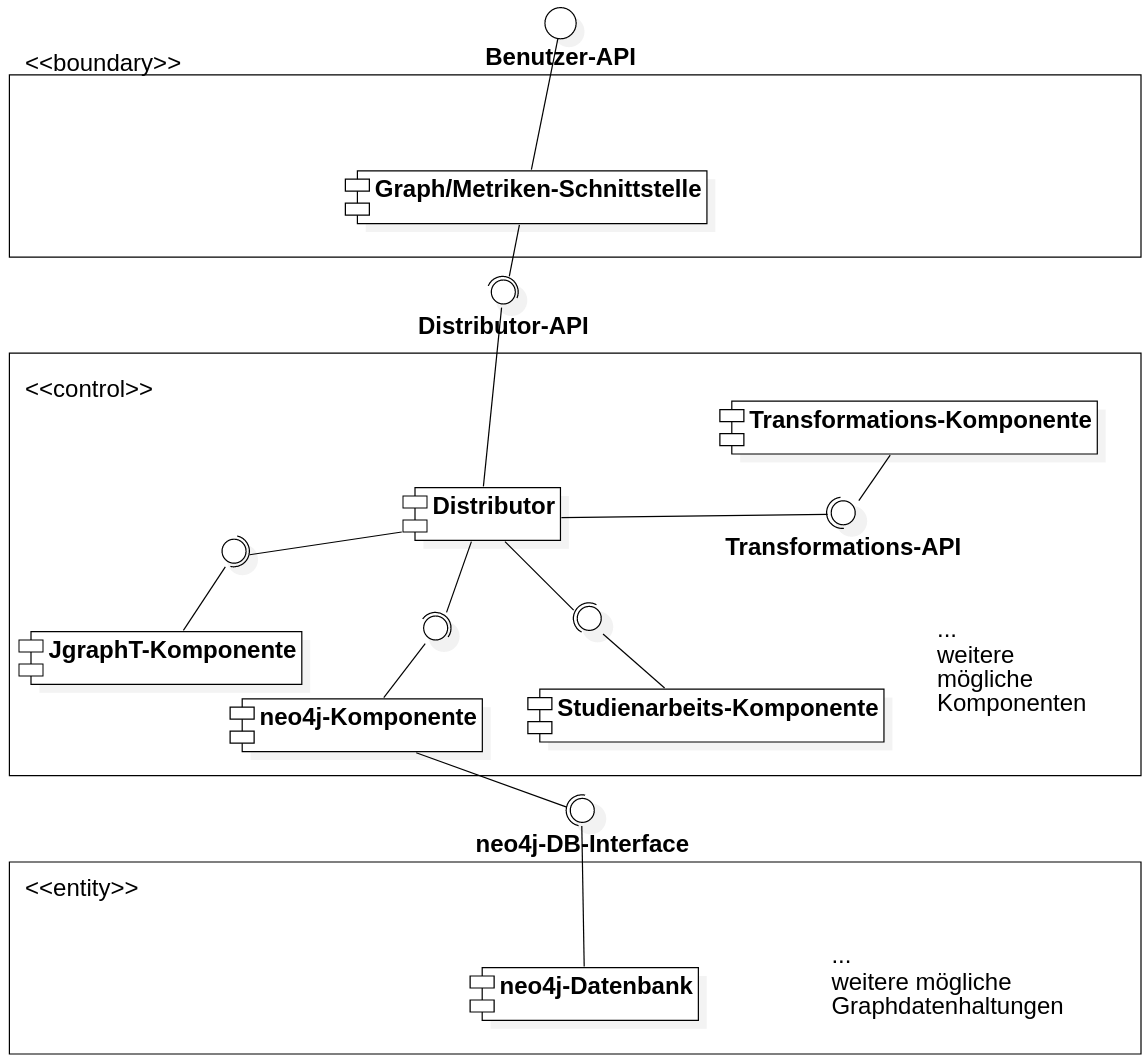
\includegraphics[scale=.38]{Abbildungen/UML/component_abstraction.png}
	\caption[Komponentendiagramm: Konzeption zur Abstraktion der Graphmetrik-Berechnung]{Komponentendiagramm: Konzeption zur Abstraktion der Graphmetrik-Berechnung}
\end{figure}
Die aufgezeigten Komponenten zeigen einzig und allein eine mögliche Konzeption und Aufgabenteilung zur Lösung des Abstraktionsproblems. Wie die konkrete Umsetzung einer solchen Software auszusehen hat, ist schlussendlich davon abhängig, wie sie eingesetzt werden soll. Weiterhin wird durch die Lösung auch nicht geklärt, wie damit umgegangen wird, wenn bestimmte Funktionen nur in machen Berechnungskomponenten vorhanden sind.

Möchte man nun den gegebenen Grobentwurf umsetzten, lassen sich verschiedene Konzepte verfolgen. Die offensichtlichste Umsetzung erfolgt mittels eines normalen Programms, dass alle Komponenten in sich vereint. In diesem Sinne ähnelt die Klassenbibliothek aus Kapitel 3 der gezeigten Abstraktion. Denn auch in der erstellten Bibliothek wurde die Metriken-Berechnung über eine Schnittstelle abstrahiert, sodass die Implementierung für den Anwender oder die Anwenderin irrelevant ist. Setzt man die Abstraktion der Graphmetrik-Berechnung allerdings als ein zusammenhängendes Programm um, ergeben sich Probleme die adressiert werden müssen. Zunächst können nur Berechnungskomponenten in das Programm z.B. als Bibliothek eingebunden werden, wenn diese mit der Technologie kompatibel sind, in der das Programm geschrieben ist. So kann es sein, dass eine C++-Bibliothek zur Berechnung von Graphmetriken nicht Teil eines Java-Programms sein kann. Des Weiteren muss noch ein Mechanismus zur Verfügung gestellt werden, der eine einheitliche und transformierbare Graphdatenstruktur zur Verfügung stellt, die für die "`Benutzer-API"' verwendet werden kann.

Eine weitere Möglichkeit zur Umsetzung des Grobentwurfes wäre es die die jeweiligen Komponenten als eigenständige Programme wahrzunehmen. Dies bietet unter anderem den Vorteil, dass man technisch nicht eingeschränkt ist, solange die Schnittstellen für jeden Teil des Systems klar definiert und ansprechbar sind. So können z.B. Berechnungs-Logiken verschiedenster Sprachen verwendet werden, ohne dass dabei Kompatiblitätsprobleme entstehen. Allerdings würde sich die Komplexität des gesamten Systems deutlich erhöhen. Jede einzelne Komponente benötigt eine eigenständige API, die in der Lage ist, nach außen zu kommunizieren. Infolgedessen müssen vor allem die angebunden Klassenbibliothek erweitert werden, sodass sie als eigenständiger Service angesprochen werden können. Die Kommunikation zwischen den einzelnen Komponenten kann sehr divers sein, solange die Kommunikationswege und die Schnittstellen klar sind. Möglich wäre eine Kommunikation über REST oder SOAP, wobei jeweils das HTTP-Protokoll verwendet wird. Ansonsten sind auch sämtliche andere Arten der Netzwerkkommunikation möglich wie Sokets oder XML-RPC. \cite{balzert_lehrbuch_2011} Alternativ kann auch auf eine Message Oriented Middleware (MOM) zurückgegriffen werden. Dies ist eine Software, die speziell dafür designed ist Nachrichten zwischen Applikationen zu verschicken \cite{curry_message-oriented_2005}. MOM und Netzwerkkommunikation können auch beliebig miteinander kombiniert werden. Auch bei der Umsetzung mittels eigenständiger Programme kommt aber noch das Problem auf, dass eine zusätzliche einheitliche Graphdatenstruktur braucht, die in die jeweiligen Strukturen der Datenbanken und Graph-Bibliotheken tranformiert werden kann. Zusätzlich muss bei der Kommunikation über die Schnittstellen ein Format gefunden werden, über das kommuniziert wird.
}
\chapter{Fazit und Ausblick}
{
Zum Ende der Studienarbeit sollen die Inhalte noch einmal zusammengefasst und wiederholt werden. Besonders wird zu der in 1.2 gestellten Fragestellungen herausgearbeitet, wie diese beantwortet wurden. Dies dient vor allem dazu ein Fazit zur Arbeit zu ziehen. Abschließend wird noch ein Ausblick zum erarbeiteten Inhalt erstellt, der aufzeigt, welche Themen aufbauend auf dieser Arbeit betrachtenswert sind.
}
\section{Fazit und Zusammenfassung der Studienarbeit}
{
Im ersten Teil der Studienarbeit wurden verschidenste Graphmetriken betrachtet und untersucht. Dabei wurde sich zusätzlich die Frage gestellt, wie die gefundenen Metriken zu kategorisieren und wie diese laufzeittechnisch und in ihrer Verbreitung zu bewerten sind. Insgesamt wurden die recherchierten Metriken in acht Kategorien unterteilt. Diese Kategorien sind:
\begin{myitemize}
	\item Grundlegende Metriken (Ordung, Größe, Grad eines Knoten etc.)
	\item Distanzmetriken (Distanz, Radius, Durchmesser)
	\item Kreis-basierte Metriken (Taillenweite, Umfang)
	\item Zusammenhangsmetriken (Vertex/Edge Connectivity, Dichte)
	\item Zentralitätsmetriken
	\item Chromatische Zahl und chromatischer Index
	\item Arborizität
	\item Weitere Metriken (nicht kategorisiert)
\end{myitemize}
Bei der Bewertung der einzelnen Metriken wurde bei der Laufzeit darauf geachtet, ob die Berechnung der Metrik ein effizient lösbares Problem ist oder nicht. Bei einigen Metriken (chomatische Zahl, chromatischer Index, Unabhängigkeitszahl) kam dabei heraus, dass sie nicht effizient berechnenbar sind. Bei Bewertung der Verbreitung wurde vor allem das Vorhandensein in einschlägigen Mathematikbibliotheken (MatLab, SageMath, Wolfram) der Metriken betrachtet. Eine Übersicht über alle Metriken und ihre Definition ist in Abschnitt 2.9 gegeben.

Anschließend zur Untersuchung der Graphmetriken wurde betrachtet, wie sich die beschriebenen Kennzahlen innerhalb einer Klassenbibliothek umgesetzt werden können. Hierfür wurde sich zunächst die Frage gestellt, welche Anforderungen eine solche Software hat. Um diese Fragestellung zu lösen wurde sich an der Anfroderungsanalyse orientiert, die Helmut Balzert in seinem "`Lehrbuch der Softwaretechnik"' beschreibt \cite{balzert_lehrbuch_2009}. So wurden zunächst grobe Ziele für die Bibliothek definiert. Dann konnten die Rahmenbedingungen der Software festgehalten werden. Entstanden ist eine Java-Klassenbibliothek, die als Maven-Artifakt verwendet werden kann. Dabei stellt die Software eine Graphdatenstruktur und die Berechnung diverser Graphmetriken zur Verfügung. Neben diesen groben Eigenschaften und Zielen wurden detailiert Anforderungen für die Graphdatenstruktur und die Graphmetriken erarbeitet. Auch wurden nicht funktionale Anforderungen definiert. Dazu zählen "`Usability"', Angemessenheit, Genauigkeit, Wartbarkeit und Portabilität. Auf Basis der Anforderungen konnten Use Cases erstellt werden, die die Klassenbibliothek abdecken sollen. Zu dem entstandenen Use Case-Diagramm wurden zudem Use Case-Schablonen erstellt. Zum Abschlus der Studienarbeit sind noch Analysen zur Persistierung eines Graphen und zur Implementierung der Graphdatenstruktur vorgenommen worden, um ausreichend Wissen für den Programmentwurf zu sammeln.

Im Anschluss an die Analysephase wurde der Entwurf für die Klassenbibliothek erarbeitet. Zu Beginn wurde der statische Entwurf vorgestellt. Hierbei wird die Graphdatenstruktur durch ein Interface rerpäsentiert. Dieses Interface wird durch zwei Klassen implementiert, wobei eines einen gerichteten das andere einen ungerichteten Adjazenzlistengraph implementiert. Um kein Codedopplungen zu erzeugen, erben beide Klassen von der abstrakten Klasse \textit{AdjacencyListGraph}, die alle identischen Methoden beider Implementierungen und die eigenltichen Adjazenzlisten hält. Um bei der Berechnung der Graphmetriken zu unterscheiden, welche Grapharten vorliegen, wurden die Implementierungen zudem mit sogenannten "`Marker"'-Interfaces markiert.

Zu Berechnung der Graphmetriken stellt die statische Struktur eine vereinfachte Schichtenarchitketur zur Verfügung. Der Nutzer oder die Nutzerin können über eine einheitliche Schnittstelle die Berechnung der vorhanden Metriken einleiten. Die Metriken selbst werden durch Enumerationen identifiziert. In speziellen Berechnungsklassen, die die Metriken-Kategorien aus Kapitel 2 wiederspiegeln, finden sich dann die Algorithmen zur Ermittlung der Metriken. Sämtliche Methoden zur Berechnung der Graphkennzahlen sind statische Methoden, um den funktionalen Charakter der Berechnung zu verdeutlichen und um unnötige Objekterzeugungen zu vermeiden. Neben dem statischen Entwurf wurde auch auf dynamische Aspekte der Bibliothek eingegangen. Es wurde gezeigt, wie die Graphdatenstruktur erstellt und manipuliert werden kann und wie der Workflow einer Graphmetrik-Berechnung abläuft. Im Anschluss wurde ausführlich gezeigt, wie die einzelnen Metriken algorithmisch umgesetzt wurden. Hierbei wurde auch auch sprachspezifische Aspekte eingegangen und die Algorithmen nicht nur schematisch dargestellt.

Zur Sicherstellung der Korrektheit und Einhaltung der nicht funkionalen Anforderungen wurde auch gezeigt, wie die Klassenbibliothek getestet wurde und welche Designentscheidungen getroffen wurden, damit die nicht funkionalen Anforderungen eingehalten worden sind.

Im letzten Kapitel der Studienarbeit wurde sich damit beschäftigt, wie die Berechnung der Graphmetrik programmatisch so umkonstruiert werden kann, sodass die Berechnung mit einem beliebigen "`Backend"' stattfinden kann, allerdings die Schnittstelle zur Berechnung einheitlich ist. Ein "`Backend"' kann dabei eine weitere Klassenbibliothek sein oder z.B. eine Graphdatenbank. Zur Lösung dieses Abstraktionsproblems wurde eine Schichtenarchitketur vorgeschlagen, bei der ein oder mehrere Komponenten als einheitliche Schnittstelle fungieren. ZUr Repräsentation des Graphen wird zudem ein einheitliches Format benötigt. Auf einer weiteren Ebene wird die eigentliche Berechnung durchgeführt. Hierbei wird der einheitliche Graph zunächst in das jeweilige Format des gewählten "`Backends"' umgewandelt und anschließend analysiert. In einer dritten Schicht sind ggf. Graphdatenbanken oder andere Persistierungsprogramme enthalten. Zur Umsetzung dieses Grobentwurfes wurde vorgeschalgen dies innerhalb eines großen Programmes zu realsieren, wobei es zu Kompatiblitätsproblemen kommen kann. Alternativ können die einzelnen Komponenten eigenständige Programme sein, die über eine Schnittstelle angesprochen werden können. Die Kommunikation zwischen den Komponenten kann dann über Netzwerkprotokolle oder MOM geschehen.
}
\section{Ausblick}
{
Im Rahmen dieser Arbeit konnte der Sachverhalt der Graphmetriken und deren programmatische Umsetzung in einem hohen Detail beleuchtet werden. Aufbauend auf den vorliegenden Ergebnissen können weitere Fragestellungen formuliert werden, die beispielsweise in Folgestudienarbeiten beantwortet werden können. 

Wie in Kapitel 4 gezeigt, stellt die Studienarbeit die Frage auf, wie es möglich ist die Berechnung der Graphmetriken weiter zu abstrahieren. Die Arbeit selbst gibt einen groben Entwurf, bzw. eine grobe Idee darüber, wie es möglich wäre diese Abstraktion umzusetzen. Auch werden bestimmte konkrete Lösungsansätze skizziert. Allerdings steht die Frage noch offen, wie eine reale Umsetzung dieser Abstraktion tatsächlich aussehen könnte und ob der Vorgeschlagene Entwurf überhaupt so umsetzbar ist. Dieser Aspekt der Abstraktion könnte noch weiter untersucht werden.

Eine weitere Methode Graphmetriken anzuwenden, könnte darin bestehen mit ihnen zu versuchen die Ähnlichkeit von Graphen zu untersuchen. Genauer gesagt, wäre es erstrebenswert, wenn es mit Hilfe von Graphmetriken möglich wäre herauszufinden, ob zwei Graphen sich stark oder weniger stark ähneln in dem Sinne, dass ihre Struktur gleich ist. Auch für diese Anwendung gibt es viele Realweltprobleme, die Nutzen daraus ziehen können. So ist es beispielsweise möglich in chemischen Datenbanken noch ähnlichen Strukturen zu suchen. Im Rahmen dessen gab es schon viel Forschung in die Richtung die Isomorphie von Graphen herauszufinden. Im Rahmen der Isomorphie hat sich auch der Begriff der "`vollständigen"' Graphinvariante etabliert. Ist eine Graphmetrik vollständig, so gibt diese eindeutig bei gleichem Wert an, ob zwei Graphen zueinander isomorph sind. Da allerdings das Kriterium der Isomorphie oft sehr streng ist, ist es vor allem noch wichtig weitere Ähnlichkeitsmaße zu definieren, wobei auf die große Anzahl an Graphinvarianten zurückgegriffen wird. Diese Entwicklung verschiedener Ähnlichkeitsmaße und die Bewertung dieser könnte noch Teil weiterer Untersuchungen werden. \cite{dehmer_computational_2014,zager_graph_2008}
}
\chapter*{Glossar}
\addcontentsline{toc}{chapter}{Glossar}
{
\geintrag{Graph}{Ein Paar bestehend auf Knoten V und Kanten E. \(G=(V,E), \text{wobei }E\subseteq V\times V\))}
\geintrag{Graph-Invariante}{Eine Funktion, die einen Graphen auf eine Zahl abbildet. Sind zwei Graphen isomorph so wird ihnen der gleiche Wert zugewiesen. \cite{diestel_graphentheorie_2000}}
\geintrag{Graph-Metrik}{siehe \textit{Graph-Invariante}}
}
\printbibliography
\end{document}